%%%%%%%%%%%%%%%%%%%%%%%%%%%%%%%%%%%%%%%%%%%%%%%%%%%%%%%%%%%%%%%%%
% Contents: Main Input File of the LaTeX2e Introduction
% $Id$
%%%%%%%%%%%%%%%%%%%%%%%%%%%%%%%%%%%%%%%%%%%%%%%%%%%%%%%%%%%%%%%%%
% lshort.tex - The not so short introduction to LaTeX   
%                                                      by Tobias Oetiker
%                                                     oetiker@ee.ethz.ch
%
%                           based on LKURTZ.TEX Uni Graz & TU Wien, 1987
%-----------------------------------------------------------------------
%
% To compile lshort, you need TeX 3.x, LaTeX and makeindex
%
% The sources files of the Intro are:
%      lshort.tex (this file),
%      titel.tex, contrib.tex, biblio.tex
%      things.tex, typeset.tex, math.tex, lssym.tex, spec.tex,
%      lshort.sty, fancyheadings.sty
%
% Further the  verbatim.sty and the layout.sty 
% from the LaTeX Tools distribution is
% required.
%
%
% To print the AMS symbols you need the AMS fonts and the packages
% amsfonts, eufrak and eucal from (AMS LaTeX 1.2)
%
% ---------------------------------------------------------------------

%%%%%%%%%%%%%%%%%%%%%%%%%%%%%%%%%%%%%%%%%%%%%%%%%%%%%%%%%%%%%%%%%
% Contents: Who contributed to this Document
% $Id$
%%%%%%%%%%%%%%%%%%%%%%%%%%%%%%%%%%%%%%%%%%%%%%%%%%%%%%%%%%%%%%%%%
%\begin{small} 
%  \noindent Copyright \copyright 2019 Raid Al-Nima and Contributors.  All rights reserved.
% 
%  This document is free; you can redistribute it and/or modify it
%  under the terms of the GNU General Public License as published by
%  the Free Software Foundation; either version 2 of the License, or
%  (at your option) any later version.
%  
%  This document is distributed in the hope that it will be useful, but
%  \emph{without any warranty}; without even the implied warranty of
%  \emph{merchantability} or \emph{fitness for a particular purpose}\@.  See the GNU
%  General Public License for more details.
%
%\end{small}

\chapter{Thank you!}

\begin{verse}
\contrib{Raid Rafi Omar Al-Nima}{raidrafi1@gmail.com}%
{Technical Engineering College of Mosul, Northern Technical University, Iraq}
\contrib{Tingting Han}{tingting@dcs.bbk.ac.uk}%
{Department of Computer Science and Information Systems, Birkbeck, University of London}
\contrib{Taolue Chen}{t.chen@dcs.bbk.ac.uk}%
   {Department of Computer Science and Information Systems, Birkbeck, University of London}
``RC grant EP/P015387/1".
\end{verse}

%\newpage \noindent The
%following individuals helped with corrections, suggestions and
%material to improve this paper. They put in a big effort to help me
%get this document into its present shape. I would like to
%sincerely thank all of them. Naturally, all the mistakes you'll find
%in this book are mine. If you ever find a word that is spelled
%correctly, it must have been one of the people below dropping me a
%line.
%
%If you want to contribute to this booklet, you can find all the source code
%on \url{https://github.com/oetiker/lshort}. Your pull requests will be
%appreciated.
%
%{\flushleft\small
%Eric~Abrahamsen,        % <eric@ericabrahamsen.net>
%Lenimar~Nunes~de~Andrade, % <lenimar@mat.ufpb.br> 12 Nov 1999
%Eilinger~August,        % <eaugust@student.ethz.ch>
%Rosemary~Bailey,        % <r.a.bailey@qmw.ac.uk> 0.2
%Barbara~Beeton,         % <bnb@ams.org>
%Marc~Bevand,            % <bevand_m@epita.fr>
%Connor~Blakey,          % it's Ligatures!
%Salvatore~Bonaccorso,   % <bonaccos@ee.ethz.ch>
%Pietro~Braione,         % <braione@elet.polimi.it>
%Friedemann~Brauer,      % <fbrauer@is.dal.ca> 3.4
%Markus~Br\"uhwiler,     % <m.br@switzerland.org>
%Jan~Busa,               % <busaj@ccsun.tuke.sk>
%David~Carlisle,         % GONE <carlisle@cs.man.ac.uk> 1.0
%Neil~Carter,            % <n.carter@Swansea.ac.uk>
%Carl~Cerecke,           % <cdc@cosc.canterbury.ac.nz>
%Mike~Chapman,           % <chapman@eeh.ee.ethz.ch> 3.16
%Pierre~Chardaire,       % <pc@sys.uea.ac.uk>
%Xingyou~Chen,           % <niatlantice@gmail.com> 5.04
%Christopher~Chin,       % <chris.chin@rmit.edu.au> 3.1
%Diego~Clavadetscher,    % <dc@clavatax.ch>
%Wim~van~Dam,            % GONE <wimvdam@cs.kun.nl> 2.2
%Benjamin~Deschwanden    % <vdeschwb@student.ethz.ch>
%Jan~Dittberner,         % <jan@jan-dittberner.de> 3.15
%Michael~John~Downes,    % <mjd@ams.org> 14 Oct 1999
%Matthias~Dreier,        % <dreier@ostium.ch>
%David~Dureisseix,       % <dureisse@lmt.ens-cachan.fr> 1.1
%Hans~Ehrbar,            % <ehrbar@econ.utah.edu>
%Elliot,                 % GONE <enh-a@minster.york.ac.uk> 1.1
%Rockrush~Engch,         % <niatlantice@gmail.com>
%William~Faulk,          % <wfaulk@webassign.net>
%Robin~Fairbairns,       % <robin.fairbairns@cl.cam.ac.uk> 0.2 1.0
%Johan~Falk,             % <johan@vaxjonexus.com> 5.0.1
%J\"org~Fischer,         % <j.fischer@xpoint.at> 3.16
%Frank~Fischli,          % <fischlifaenger@gmx.ch>
%Daniel~Flipo,           % <daniel.flipo@univ-lille1.fr>
%Frank,                  % <frank@freezone.co.uk> 11 Feb 2000
%Mic~Milic~Frederickx,   % <mic.milic@web.de>
%David~Frey,             % <david@eos.lugs.ch> 2.2
%Erik~Frisk,             % <frisk@isy.liu.se> 3.4
%Hans~Fugal,             % <hans@fugal.net>
%Robert~Funnell,         % <robert.funnell@mcgill.ca> 5.1
%Greg~Gamble,            % <gregg@maths.uwa.edu.au> 2.2
%Andy~Goth,              % <unununium@openverse.com>
%Cyril~Goutte,           % <goutte@ei.dtu.dk> 2.1 2.2
%Kasper~B.~Graversen,    % <kbg@dkik.dk>
%Arlo~Griffiths,         % <a.griffiths@let.leidenuniv.nl>
%Alexandre~Guimond,      % <guimond@iro.umontreal.ca> 0.9
%Neil~Hammond,           % <nfh@dmu.ac.uk> 0.3
%Christoph~Hamburger,    % <ch.hamburger@gmail.com>
%Rasmus~Borup~Hansen,    % GONE <rbhfamos@math.ku.dk> 0.2 0.9 0.91 0.92 1.9.9
%Joseph~Hilferty,        % <hilferty@fil.ub.es>
%Daniel~Hirsbrunner,     % <dhirsbrunner1@gmail.com>
%Martien~Hulsen,         % <m.a.hulsen@Wbmt.tudelft.nl> 1.0 1.1
%Bj\"orn Hvittfeldt,     % <bjorn@hvittfeldt.com> 3.13
%Morten~H\o gholm,       % <morten.hoegholm@latex-project.org>
%Werner~Icking,          % <werner.icking@gmd.de> 3.1
%Eric~Jacoboni,          % GONE <jacoboni@enseeiht.fr> 0.1 0.9
%Jakob,                  % <diness@get2net.dk>
%Alan~Jeffrey,           % <alanje@cogs.sussex.ac.uk> 0.2
%Martin~Jenkins,         % xqp.ltd@gmail.com 5.04
%Byron~Jones,            % <bj@dmu.ac.uk> 1.1
%David~Jones,            % GONE <djones@ca.mcmaster.dcss.insight> 1.1
%Johannes-Maria~Kaltenbach, % <kaltenbach@zeiss.de> 3.01
%Nils~Kanning,           % <nils@kanning.de>
%Andrzej~Kawalec,        % GONE <akawalec@prz.rzeszow.pl> 1.9.9
%Christian~Kern,         % <ck@unixen.hrz.uni-oldenburg.de> 2.1
%Alain~Kessi,            % <alain_kessi@hotmail.com> 2.2
%Axel~Kielhorn,          % <a.kielhorn@web.de>
%Sander~de~Kievit,       % <Skievit@ucu.uu.nl>
%Kjetil~Kjernsmo,        % <kjetil.kjernsmo@astro.uio.no> 3.2
%Tobias~Klauser,		% <tklauser@access.unizh.ch> 4.17
%J\"org~Knappen,         % <knappen@vkpmzd.kph.uni-mainz.de> 0.1
%Michael~Koundouros,     % <mkoundouros@hotmail.com>
%Matt~Kraai,             % <matt.kraai@amo.abbott.com>
%Tobias~Krewer,          % <tobias.krewer@googlemail.com>
%Flori~Lambrechts,       % <f.lambrechts@softhome.net>
%Mike~Lee,               % <rmrstar@gmail.com>
%Maik~Lehradt,           % <greek@uni-paderborn.de> 0.1
%R\'emi~Letot,           % <r_letot@yahoo.com>
%Axel~Liljencrantz,	% <axel.liljencrantz@byv.kth.se>
%Jasper~Loy,             % <jasper.loy@gmail.com>
%Johan~Lundberg,         % <p99jlu@physto.se>
%Martin~Maechler,        % <maechler@stat.math.ethz.ch> 2.2
%Alexander~Mai,          % <alexander.mai@physik.tu-darmstadt.de> 3.8
%Claus~Malten,           % GONE <asi138%bitnet.djukfa11@bitnet.cearn> 1.1
%Kevin~Van~Maren,        % <vanmaren@fast.cs.utah.edu> 24 Nov 1999
%Pablo~Markin,
%I.~J.~Vera~Mar\'un,     % <i.j.veramarun@ewi.utwente.nl>
%Hendrik~Maryns,         % <hendrik.maryns@ugent.be>
%Chris~McCormack,        % GONE <chrismc@eecs.umich.edu> 0.1
%Aleksandar~S.~Milosevic, % <aleksandar.milosevic@yale.edu>
%Henrik~Mitsch,          % <henrik.mitsch@gmx.at>
%Stefan~M.~Moser,        % <stefan.moser@ieee.org>
%Armin~M\"uller,		% arm.in@web.de
%Philipp~Nagele,         % <philipp.nagele@t-systems.com>
%Richard~Nagy,           % <r.nagy@nameshield.net>
%Manuel~Oetiker,         % <manuel@oetiker.ch>
%Urs~Oswald,             % <osurs@bluewin.ch>
%Hubert~Partl,           % <partl@mail.boku.ac.at> 0.2 1.1
%Marcelo~Pasin,          % <pasin@di.fc.ul.pt>
%Martin~Pfister,		% <m@rtinpfister.ch>
%Lan~Thuy~Pham,          % <lan.thuy.pham@gmail.com>
%Breno~Pietracci,        % <bpietracci@gmail.com>
%Demerson~Andre~Polli,   % <polli@linux.ime.usp.br>
%Maksym~Polyakov,        % <polyama@myrealbox.com>
%Nikos~Pothitos,		% <n.pothitos@di.uoa.gr>
%John~Refling,           % <refling@sierra.lbl.gov> 0.1 0.9
%Mike~Ressler,           % <ressler@cougar.jpl.nasa.gov> 0.1 0.2 0.9 1.0 1.9.9
%Brian~Ripley,           % <ripley@stats.ox.ac.uk> 2.1
%Kurt~Rosenfeld,		% <kurt@isis.poly.edu>
%Bernd~Rosenlecher,      % <9rosenle@informatik.uni-hamburg.de> 10 Feb 2000
%Chris~Rowley,           % <c.a.rowley@open.ac.uk> 0.91
%Young~U.~Ryu,           % <ryoung@utdallas.edu> 2.1
%Risto~Saarelma,         % <risto.saarelma@cs.helsinki.fi>
%Andr{\'a}s~Salamon,     % <andras.salamon@comlab.ox.ac.uk>
%Jos\'e~Carlos~Santos,   % <jcsantos@fc.up.pt>
%Christopher~Sawtell,    % <csawtell@xtra.co.nz> 1 Sep 1999
%Gilles~Schintgen,       % <gschintgen@internet.lu>
%Craig~Schlenter,        % <cschle@lucy.ee.und.ac.za> 0.1 0.2 0.9
%Hanspeter~Schmid,       % <schmid@isi.ee.ethz.ch>
%Baron~Schwartz,         % <bps7j@cs.virginia.edu>
%Jordi~Serra~i~Solanich, % <solanich@gmail.com>
%Miles~Spielberg,        % <zeibach@hotmail.com>
%Susan~Stewart,
%Matthieu~Stigler,
%Geoffrey~Swindale,      % <geofftswin@ntlworld.com>
%Laszlo~Szathmary,       % <szathml@delfin.klte.hu>
%Boris~Tobotras,         % <tobotras@jet.msk.su>
%Josef~Tkadlec,          % <tkadlec@math.feld.cvut.cz> 2.0 2.2
%Scott~Veirs,            % <scottv@ocean.washington.edu>
%Didier~Verna,           % <verna@inf.enst.fr> 2.2
%Carl-Gustav~Werner,     % <carl-gustav.werner@math.lu.se> 11 Oct 1999, 3.16
%Fabian~Wernli,          % <wernli@iap.fr> 3.2
%Matthew~Widmann,        % <mtwdmn@gmail.com>
%David~Woodhouse,        % <dwmw2@infradead.org> 3.16
%Chris~York,             % <c.s.york@Cummins.com> 21 Nov 1999
%Rick~Zaccone,           % <zaccone@bucknell.edu> 2.2
%Fritz~Zaucker,          % <zaucker@ee.ethz.ch> 3.0
%and Mikhail~Zotov.      % <zotov@eas.npi.msu.su> 3.1
%}
%
%\vspace*{\stretch{1}}
%
%\pagebreak
%\endinput
%

% Local Variables:
% TeX-master: "lshort2e"
% mode: latex
% mode: flyspell
% End:

%%%%%%%%%%%%%%%%%%%%%%%%%%%%%%%%%%%%%%%%%%%%%%%%%%%%%%%%%%%%%%%%%%
% Contents: Who contributed to this Document
% $Id$
%%%%%%%%%%%%%%%%%%%%%%%%%%%%%%%%%%%%%%%%%%%%%%%%%%%%%%%%%%%%%%%%%

% Because this introduction is the reader's first impression, I have
% edited very heavily to try to clarify and economize the language.
% I hope you do not mind! I always try to ask "is this word needed?"
% in my own writing but I don't want to impose my style on you...
% but here I think it may be more important than the rest of the book.
% --baron

\chapter{Preface}

\LaTeX{} \cite{manual} is a typesetting system that is very
suitable for producing scientific and mathematical documents of high
typographical quality. It is also suitable for producing all
sorts of other documents, from simple letters to complete books.
\LaTeX{} uses \TeX{} \cite{texbook} as its formatting engine.

This short introduction describes \LaTeXe{} and should be sufficient
for most applications of \LaTeX. Refer to~\cite{manual,companion} for
a complete description of the \LaTeX{} system.

\bigskip
\noindent This introduction is split into 6 chapters:
\begin{description}
\item[Chapter 1] tells you about the basic structure of \LaTeXe{}
  documents. You will also learn a bit about the history of \LaTeX{}.
  After reading this chapter, you should have a rough understanding how
  \LaTeX{} works.
\item[Chapter 2] goes into the details of typesetting your
  documents. It explains most of the essential \LaTeX{} commands and
  environments. After reading this chapter, you will be able to write
  your first documents, with itemized lists, tables, graphics and floating bodies.
\item[Chapter 3] explains how to typeset formulae with \LaTeX. Many
  examples demonstrate how to use one of \LaTeX{}'s
  main strengths. At the end of the chapter are tables listing
  all mathematical symbols available in \LaTeX{}.
\item[Chapter 4] explains indexes,  bibliography generation and some finer points about creating PDFs.
\item[Chapter 5] shows how to use \LaTeX{} for creating graphics. Instead
  of drawing a picture with some graphics program, saving it to a file and
  then including it into \LaTeX{}, you describe the picture and have \LaTeX{}
  draw it for you.
\item[Chapter 6] contains some potentially dangerous information about
  how to alter the
  standard document layout produced by \LaTeX{}. It will tell you how  to
  change things such that the beautiful output of \LaTeX{}
  turns ugly or stunning, depending on your abilities.
\end{description}
\bigskip
\noindent It is important to read the chapters in order---the book is
not that big, after all. Be sure to carefully read the examples,
because a lot of the information is in the
examples placed throughout the book.

\bigskip
\noindent \LaTeX{} is available for most computers, from the PC and Mac to large
UNIX and VMS systems. On many university computer clusters you will
find that a \LaTeX{} installation is available, ready to use.
Information on how to access
the local \LaTeX{} installation should be provided in the \guide. If
you have problems getting started, ask the person who gave you this
booklet. The scope of this document is \emph{not} to tell you how to
install and set up a \LaTeX{} system, but to teach you how to write
your documents so that they can be processed by~\LaTeX{}.

\bigskip
\noindent If you need to get hold of any \LaTeX{} related material,
have a look at one of the Comprehensive \TeX{} Archive Network
(CTAN) sites. The homepage is at
\url{http://www.ctan.org}.

You will find other references to CTAN throughout the book, especially
pointers to software and documents you might want to download. Instead
of writing down complete URLs, I just wrote \texttt{CTAN:} followed by
whatever location within the CTAN tree you should go to.

If you want to run \LaTeX{} on your own computer, take a look at what
is available from \CTAN|systems|.

\vspace{\stretch{1}}
\noindent If you have ideas for something to be
added, removed or altered in this document, please let me know. I am
especially interested in feedback from \LaTeX{} novices about which
bits of this intro are easy to understand and which could be explained
better.

\bigskip
\begin{verse}
\contrib{Tobias Oetiker}{tobi@oetiker.ch}%
\noindent{OETIKER+PARTNER AG\\Aarweg 15\\4600 Olten\\Switzerland}
\end{verse}
\vspace{\stretch{1}}
\noindent The current version of this document is available on\\
\CTAN|info/lshort|

\endinput



%

% Local Variables:
% TeX-master: "lshort2e"
% mode: latex
% mode: flyspell
% End:

\tableofcontents
\listoffigures
\listoftables
\enlargethispage{\baselineskip}
\mainmatter
%%%%%%%%%%%%%%%%%%%%%%%%%%%%%%%%%%%%%%%%%%%%%%%%%%%%%%%%%%%%%%%%%
% Contents: Things you need to know
% $Id$
%%%%%%%%%%%%%%%%%%%%%%%%%%%%%%%%%%%%%%%%%%%%%%%%%%%%%%%%%%%%%%%%%

\chapter{Things You Need to Know}
\begin{intro}
	Road tracking is one of the most challenging topics recently. It aims to automatically guide a car through the correct track without crashing other cars or objects. Deep reinforcement learning is considered as one of the most proficient methods that can be applied to address the road tracking issue. It combines reinforcement learning and deep learning. We model the process as a Markov Decision Process (MDP), where the deep reinforcement learning starts from a state, pick the best action by optimising considered rewards and produces a new state. The new state is then utilized as a current state, and the process continues.  

Different tracking tasks were considered in the literature as:
\begin{itemize}
	\item \underline{Tracking Object:} In 2000, Grigore and Grigore proposed a tracking system controller by using a recurrent neural network with the reinforcement learning \cite{Grigore2000Reinforcement}. In 2010, Cohen and Pavlovic suggested an effective and vigorous real-time tracker. The tracker utilized the reinforcement learning and it was applied to tracking personal faces \cite{Cohen2010Reinforcement}. In 2004, Liu and Su proposed an object tracking method by exploiting the reinforcement learning. The reinforcement learning was employed here to determine the features of the tracking object \cite{Liu2004Reinforcement}. In 2017, Supan\v{c}i\v{c} and Ramanan constructed a learning policy for tracking objects. The reinforcement learning was applied to video streams to provide on-line decision \cite{Supancic2017Tracking}. 
	\item \underline{Different Tracking Issues:} In 2009, Jinlin \textit{et al.} presented a velocity tracking control approach. The authors utilized the neuro-fuzzy technique with the Q-learning in their work \cite{Jinlin2009Neurofuzzy}. In 2011, Hall \textit{et al.} illustrated a single and double pendulum tracking model. A traditional control, Bayesian computations and reinforcement learning were employed in this publication \cite{Hall2011Reinforcement}. In 2013, Sootla \textit{et al.} described a tracking periodic gene repressilator. The fitted Q iteration algorithm was applied to one dimensional signals in this study \cite{Sootla2013On}. In 2015, Wei \textit{et al.} explained tracking a maximum power for wind speed conversion systems. In this paper, a model-free Q-learning method was exploited \cite{Wei2015Reinforcement}. 
	\item \underline{Deep Leaning Tracking:} In 2017, Perot \textit{et al.} investigated tracking roads of a driving car. A deep reinforcement learning was used \cite{Perot2017End}. The main problem in this work is that the driving car oscillates around the main road track. This is due to the selected reward in this study, where it utilized the oriented angle of the road with the car speed. In 2017 and 2018, Yun \textit{et al.} approached an action-decision network (ADNet) to track objects. The ADNet is a deep reinforcement learning network and it was applied in a quite complicated way, where a pre-trained Convolutional Neural Network (CNN) was firstly employed then the reinforcement learning was utilized \cite{Yun2017Action}\cite{Yun2018Action}. 
\end{itemize}

It can be seen from the literature that the majority of tracking studies were focused on tracking object problems as in \cite{Grigore2000Reinforcement}\cite{Cohen2010Reinforcement}\cite{Liu2004Reinforcement}\cite{Supancic2017Tracking}. Other work considered different tracking tasks such as: tracking and controlling velocity \cite{Jinlin2009Neurofuzzy}, tracking periodic gene repressilator \cite{Sootla2013On}, tracking single and double pendulum \cite{Hall2011Reinforcement}, tracking maximum powers for wind speed conversion systems \cite{Wei2015Reinforcement}. Only several studies were concentrated on utilizing the deep learning in order to address tracking issues such as \cite{Yun2017Action,Yun2018Action}. 

Our work contributes to this area by suggesting an effective road tracking procedure and employing the MDP based on the deep reinforcement learning, where states are used as inputs; rewards are utilized to evaluate the tracking policy and actions are predicted to provide new states. Efficient coding for various road tracking possibilities has been considered such as turning to the left or right and recognizing crossing object(s). This study can be exploited for driving car applications such as driverless (or automatic driving). 

After the introduction, this paper is organized as follows: Section 2 states the methodology with the theoretical concepts, Section 3 discusses the results and Section 4 concludes the paper.
\begin{figure*}[!t]
	\centering
	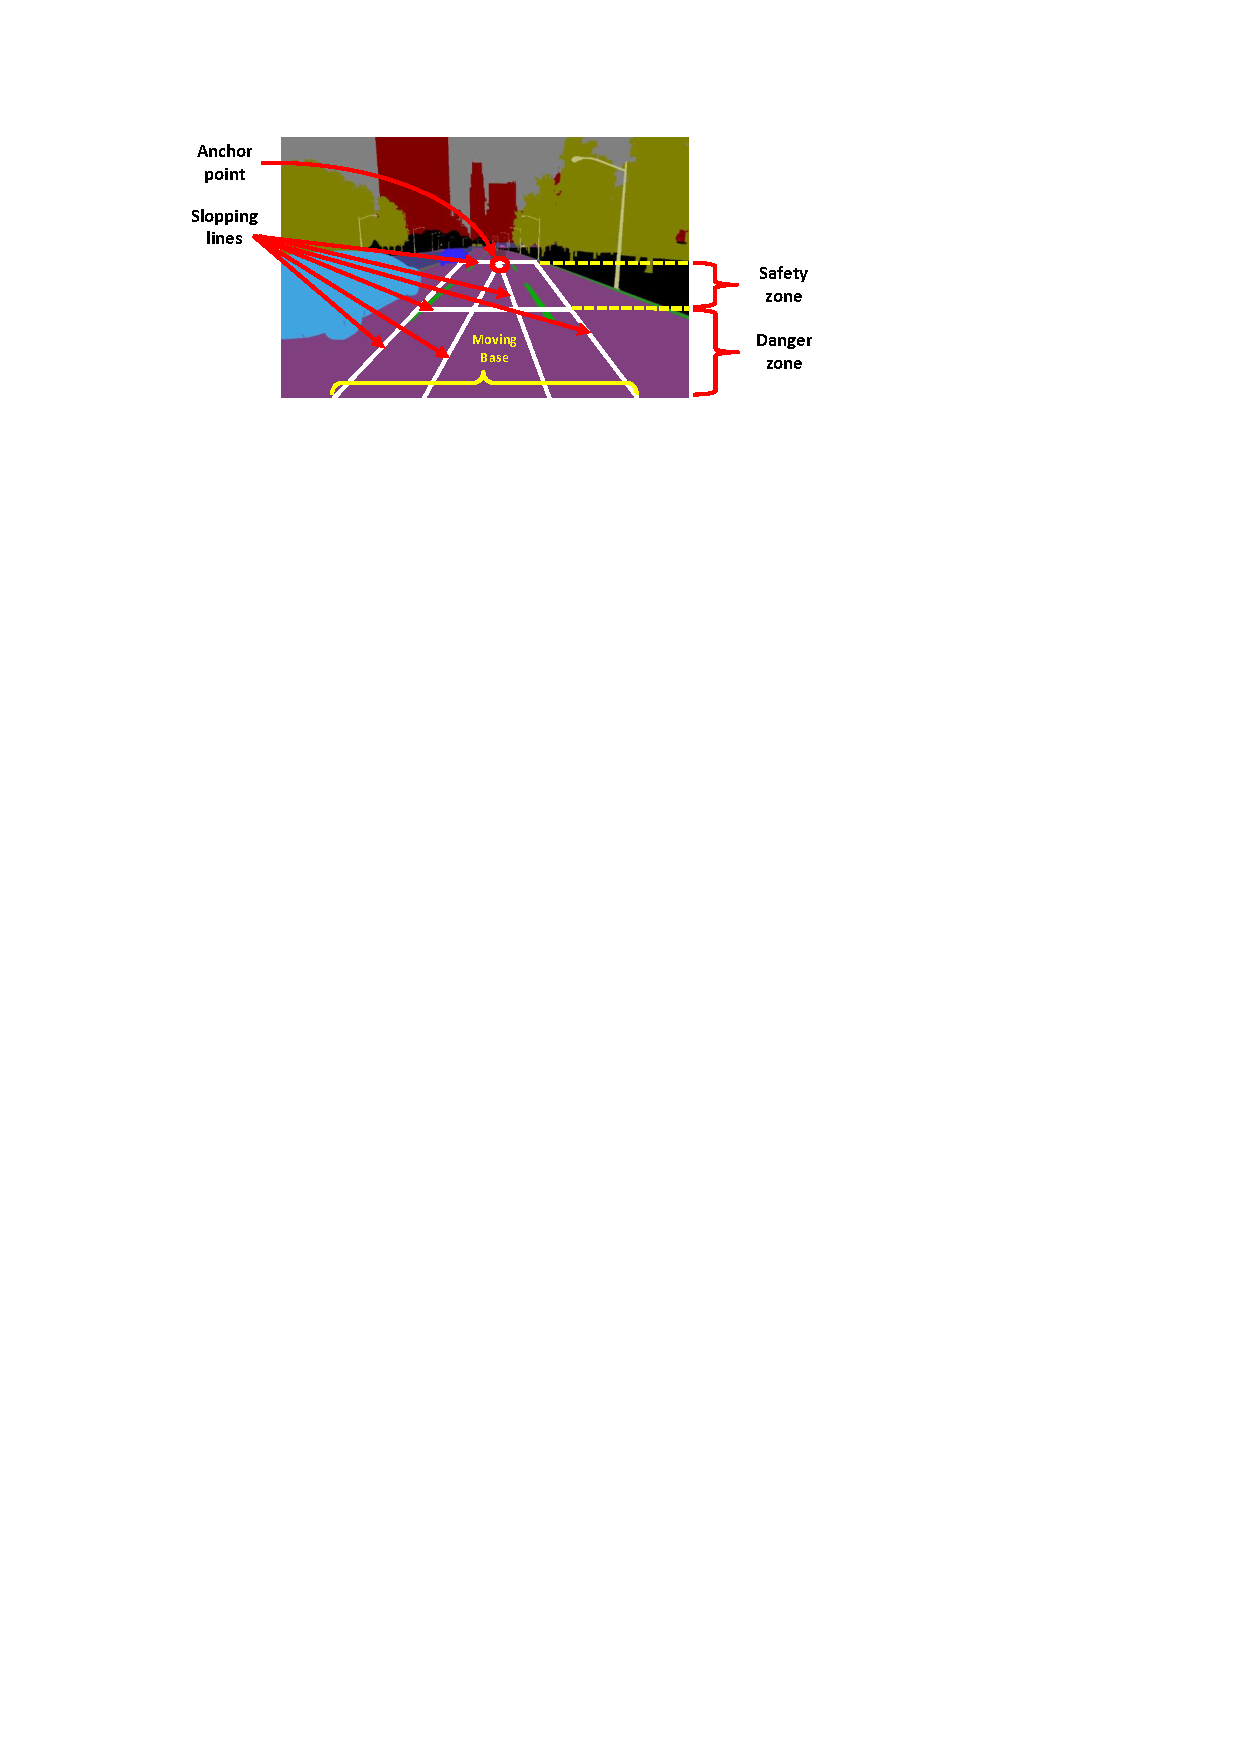
\includegraphics[scale=.9,trim=3cm 22.5cm 7.1cm 2cm,clip]{segmentation_regions2.pdf}
	\caption{The suggested front view road tracking zones, lines and anchor point}
	\label{Fig:segmentation_regions1}
\end{figure*}
\begin{figure*}[!t]
	\centering
	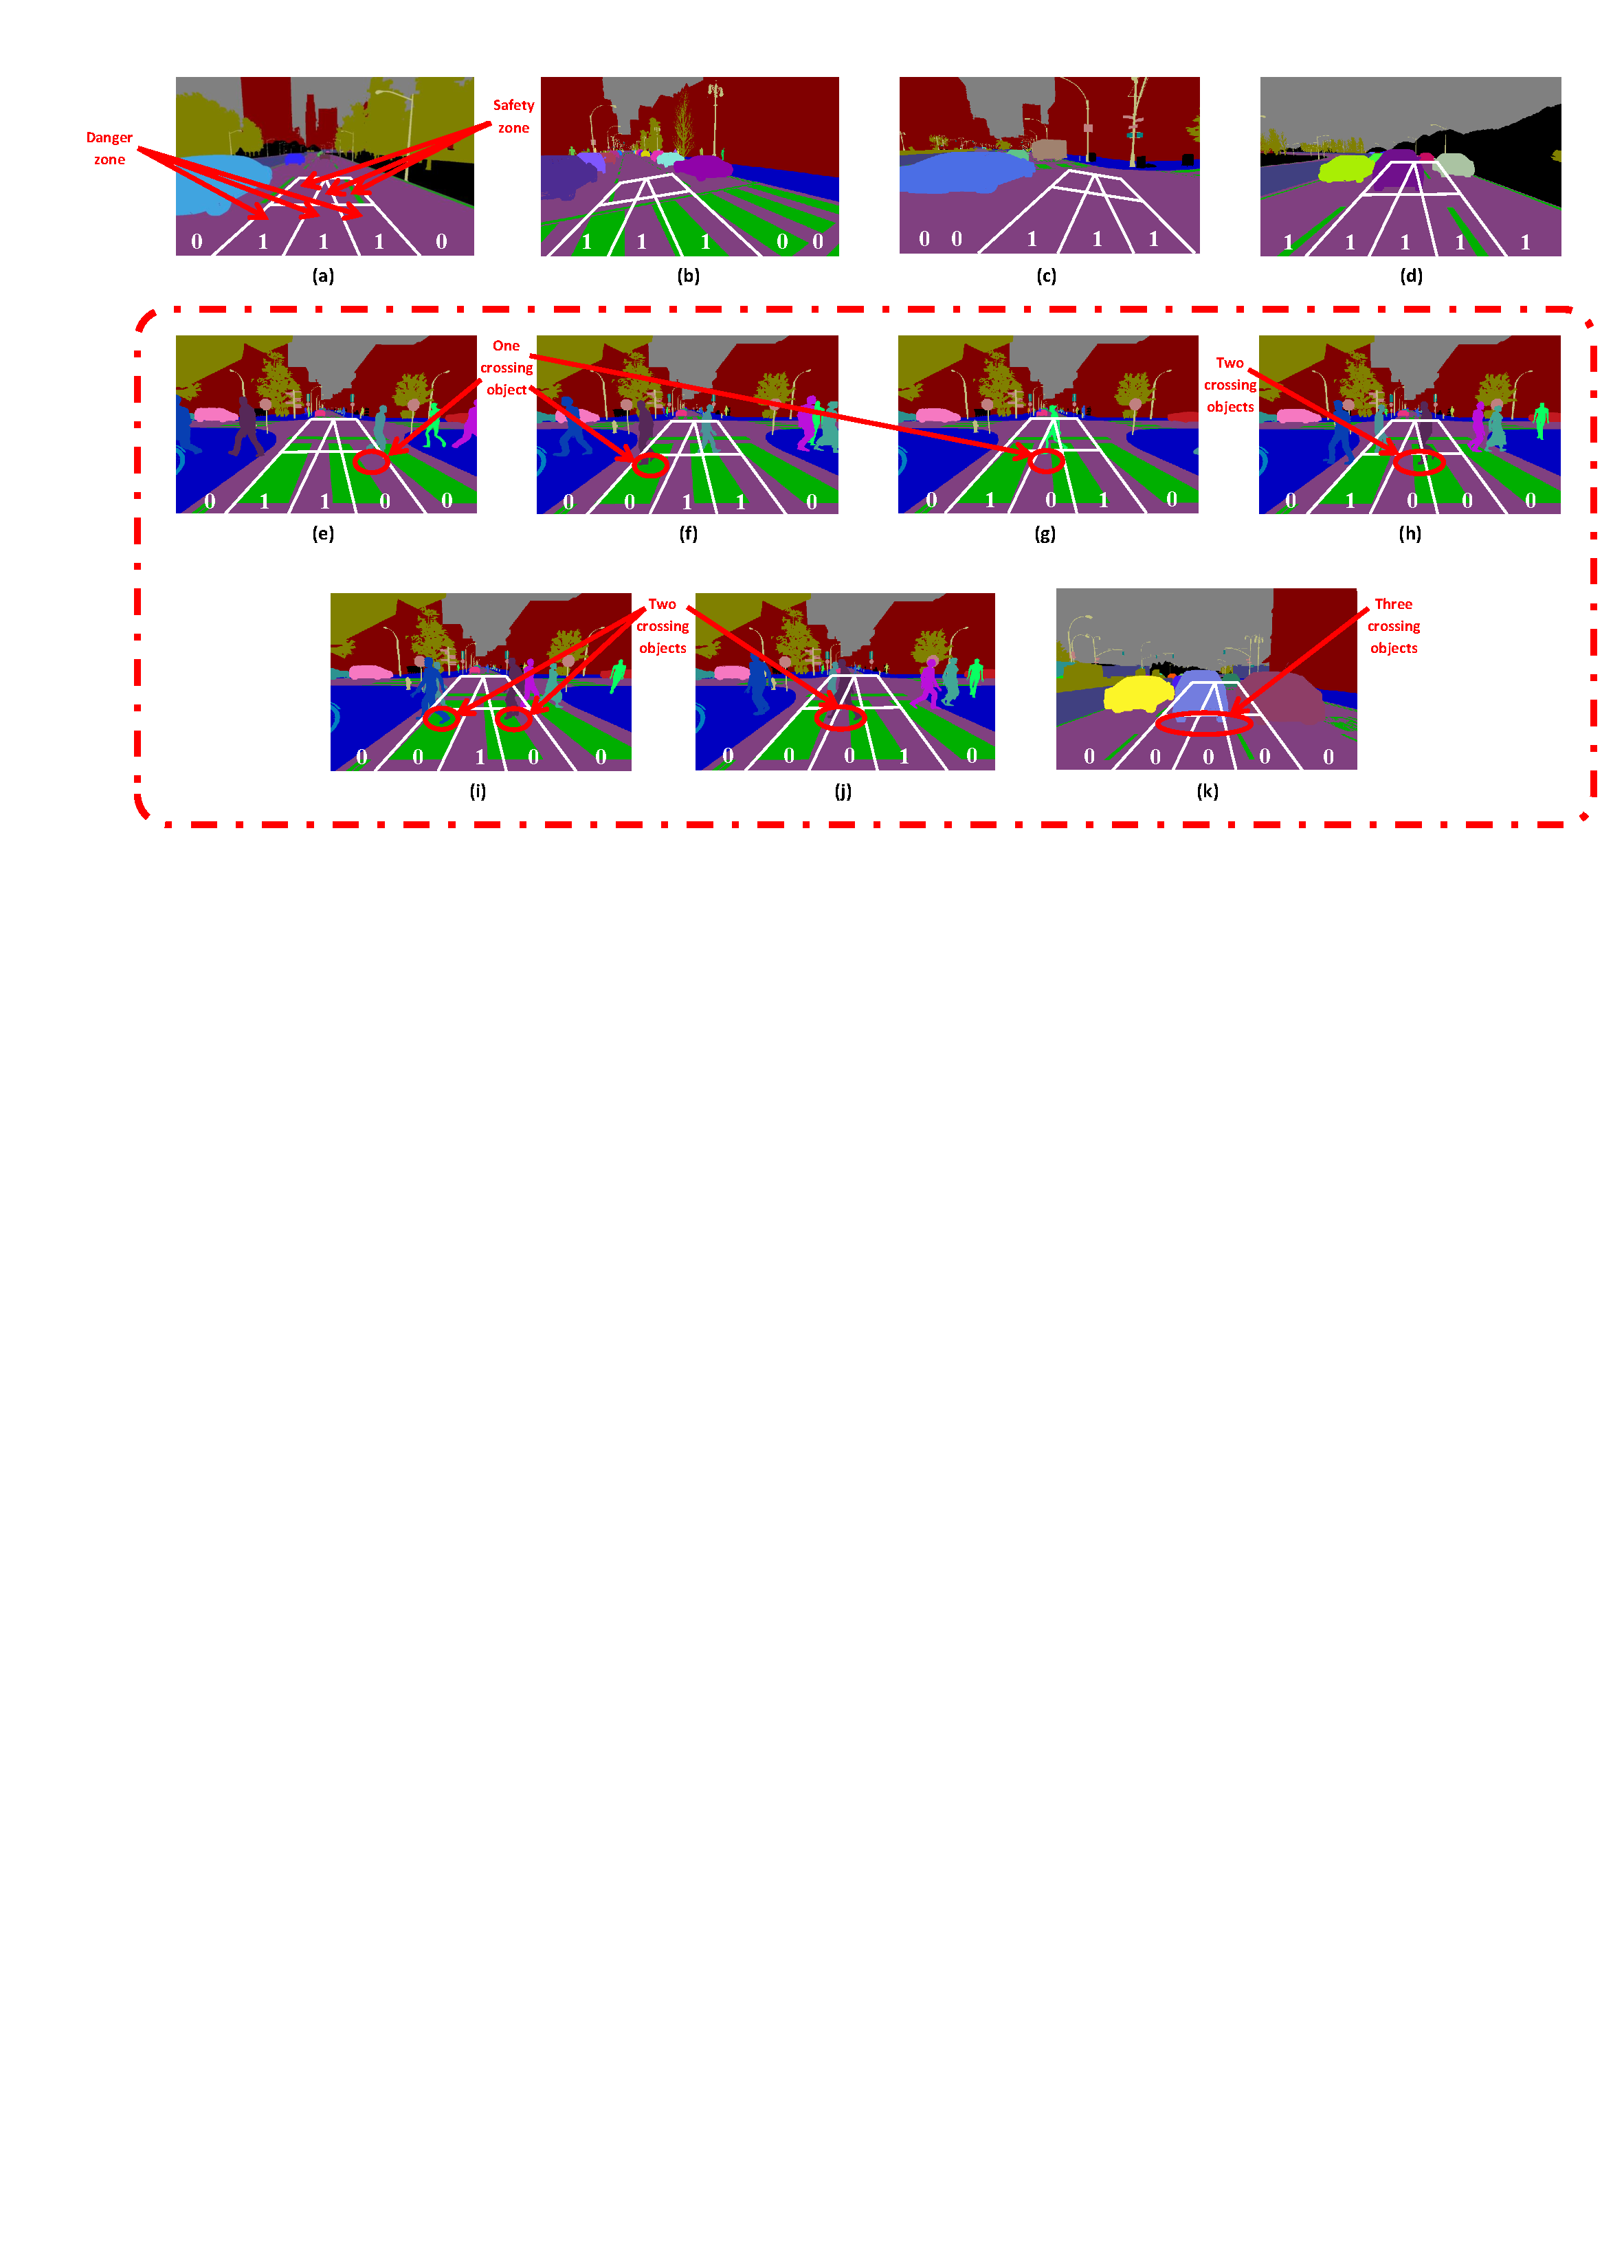
\includegraphics[scale=.4,trim=2cm 35cm 0cm 2cm,clip]{segmentation3.pdf}
	\caption{The road tracking motivations of segmented images: (a) the straight forward direction, (b) turning left direction, (c) turning right direction, (d) reverse or backward direction, (e-g) stopping action because of a single crossing object, (h-j) stopping action because of two crossing objects and (k) stopping action because of three crossing objects}
	\label{Fig:segmentation}
\end{figure*}
\begin{figure*}[!h]
	\centering
	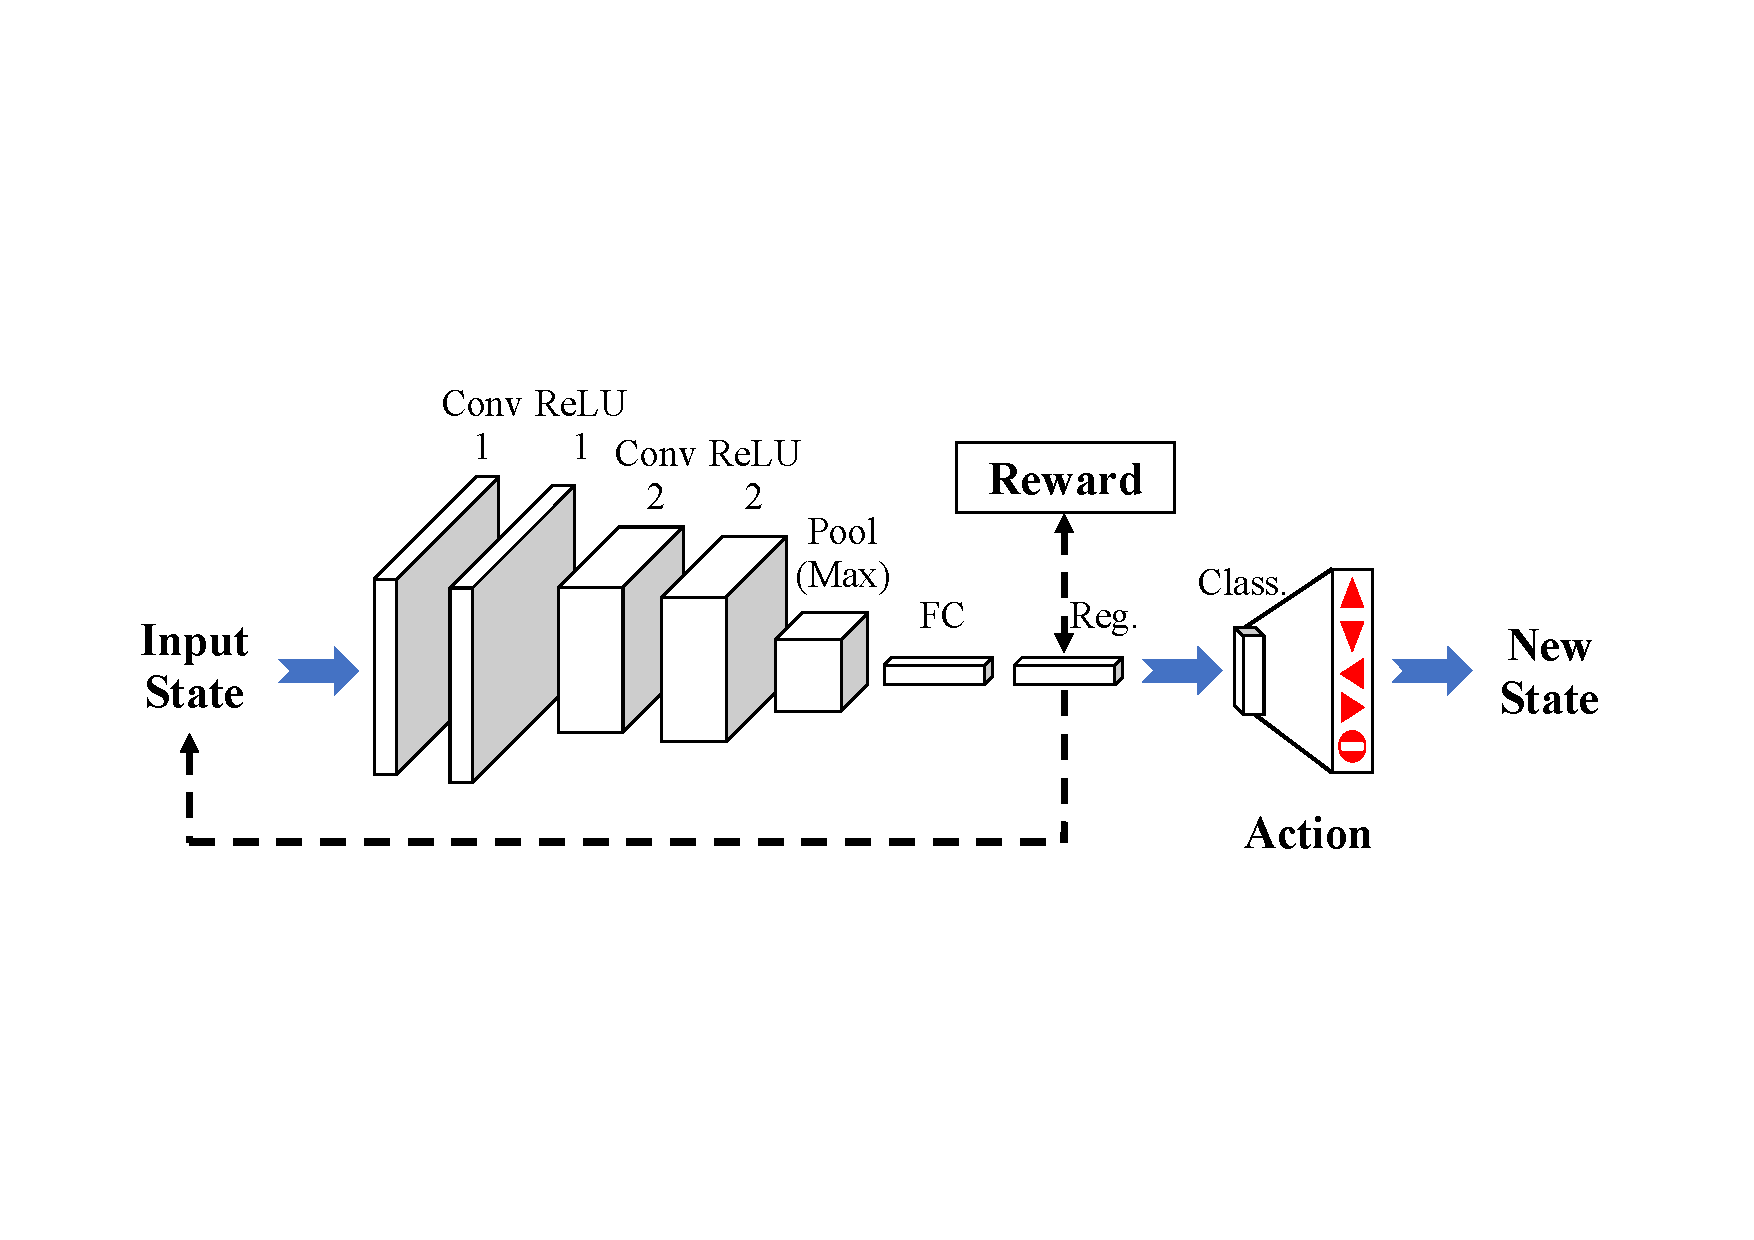
\includegraphics[scale=.65,trim=2cm 5.5cm 2cm 5.5cm,clip]{Deep_Reinf_Net1.pdf}
	\caption{The main design of the proposed DRL-RT. It consists of two conventional layers, two ReLU layers, a pooling layer, a fully connected layer, a regression layer and a classification layer}
	\label{Fig:Deep_Reinf_Net}
\end{figure*}
\end{intro}

%%%%%%%%%%%%%%%%%%%%%%%%%%%%%%%%%%%%%%%%%%%%%%%%%%%%%%%%%%%%%%%%%
% Contents: Typesetting Part of LaTeX2e Introduction
% $Id$
%%%%%%%%%%%%%%%%%%%%%%%%%%%%%%%%%%%%%%%%%%%%%%%%%%%%%%%%%%%%%%%%%
\chapter{Modelling}

\section{Modelling}
To model the road tracking, various essential issues have to be considered such as how to identify road crossing object(s), how to encode different tracking directions, how to design the deep reinforcement learning network to determine the next action, etc. Such issues will be illustrated and addressed in this section.

\subsection{Road Tracking:} 
Our research is based on the SYNTHIA-SEQS-05 database \cite{Ros2016TheSYNTHIA}. Video sequences were recorded and saved, from which one extracted front,  rear, left and right view road images around the car for both right and left steering cars. Each view covers a range of angle up to 100 degrees. As a result, a large number of simulated image frames were provided, each has a resolution of $760 \times 1,280 \times 3$ pixel. 

The images were taken in four different environments: clear
environment in spring, fog environment, rain environment and
heavy-rain environment.

In our study, we look at forward view road frames for a right steering car in all four environments. 

To differentiate the main objects on the road, specific colours were used, e.g., sky is grey, buildings are brown, roads are purple, side walks are blue and road markings are green. In other words, the purple and green colours refer to the allowed driving regions.  

More specifically, each view (image) can be divided into a safety zone and a danger zone. The safety zone is the zone that a car can keep moving to, as it is further away and it allows ample time to stop or slow down the car if necessary. The danger zone is the area that a car must stop if any objects are recognised. Such zones can be found in Fig. \ref{Fig:segmentation_regions}(e-k). 

How do we determined a safe zone or a danger zone? In each image of Fig. \label{Fig:segmentation_regions1}, a virtual triangle and trapezoid were drawn. The base of the triangle and trapezoid moves in the road direction, and the crossing lines can slope toward the tracking direction. The height of the triangle (and the trapezoid) is two thirds of the acquired image. The top one third of the trapezoid is the safety zone and the bottom two thirds is the danger zone. The shared point of the triangle and the trapezoid is called an anchor point. It denotes the road tracking direction. The anchor point can denote the direction by following the track centre. By drawing the virtual triangle in the trapezoid area is to specify three types of regions: left, right and centre. These regions can specify the direction of any crossing object. The car can, for instance, avoid an object crossing from the left side by moving to the right, if the space is empty there. If objects are identified from both sides in the danger zone, then the car has to stop.  

\subsection{Actions codes:} 
At any point, the following actions can be taken by a car: drive straight on, turn left or right, reverse and stop. In our work, we use a five-digit binary number to encode each action, see Table \ref{Table:Signs_codes}. The stop action is applied when the danger zone recognising object(s) in the way from both sides. 

When a crossing object is detected, it will change the action from that side with a ``0". For instance, the car is moving forward with action 01110, then an object appears in the danger zone from left, then the action becomes 00111. When another object appears from the right, the code will be 00110 and the car will stop. As long as there are no three consecutive 1's, the car has to stop.  We model all such cases as 00000 to reduce the number of coding values. Fig. \ref{Fig:segmentation} shows explanations for various coding cases.

The binary codes can be converted to desired equivalent codes. A standard conversion from the binary to decimal \cite{koren2001computer} is used. For instance, $(01110)_2=(14)_{10}$ and $(00111)_2=(7)_{10}$. The only exception here is the backward direction, where a negative sign (-) is added to refer to the reverse movement. It is worth mentioning that the reverse action can only be considered if the car is being out of the track. The road tracking actions with their suggested codes and descriptions are given in Table \ref{Table:Signs_codes}. The decimal codes are used in the regression layer of the proposed deep reinforcement learning network as will be explained later. They are referring to road tracking actions.

\begin{table}[!h]
	\centering
	\caption{The road tracking actions with their suggested codes and descriptions}
	\label{Table:Signs_codes}
	\begin{tabular}{|c|C{2cm}|C{2cm}|C{5cm}|}
		\hline
		\textbf{Action sign} & \textbf{Binary code} & \textbf{Equivalent decimal code} & \textbf{Description} \\ \hline
		\begin{minipage}{.075\textwidth}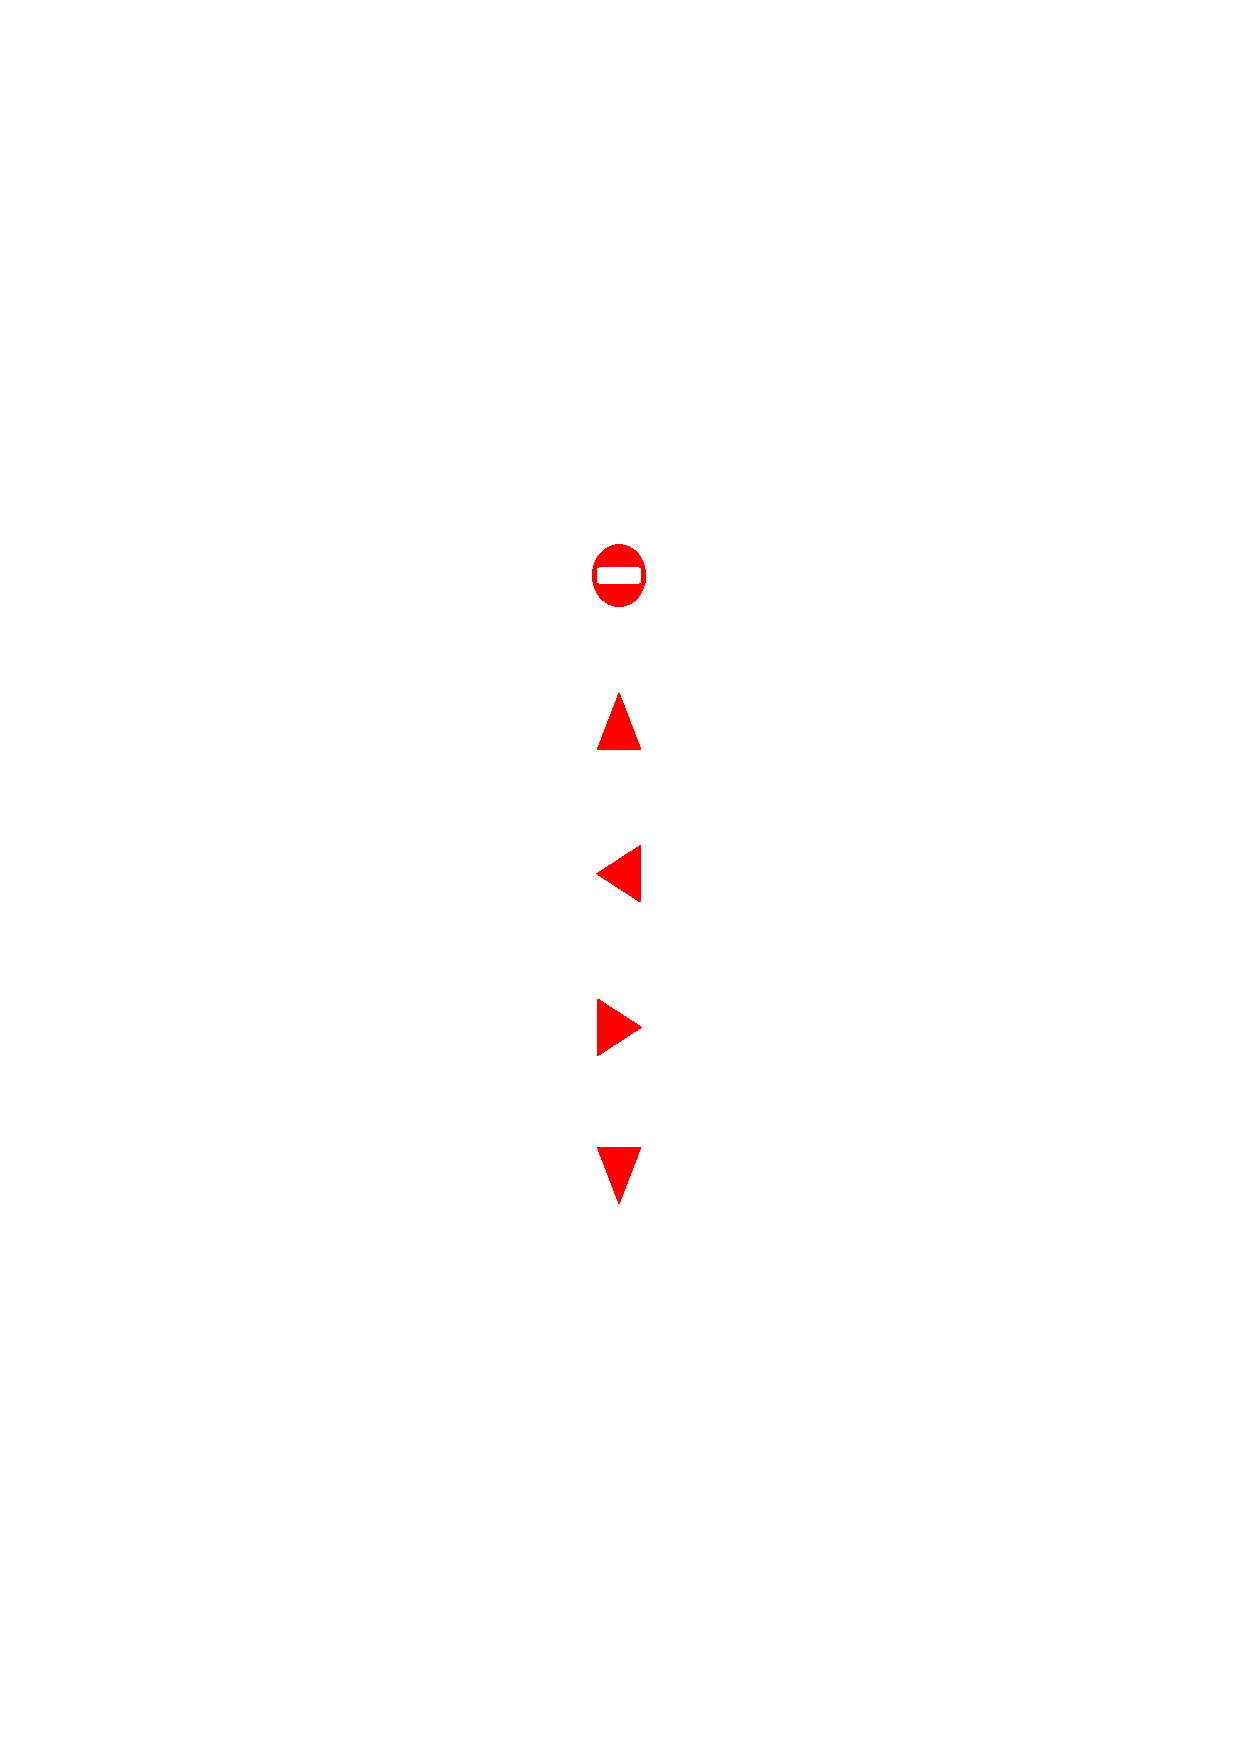
\includegraphics[scale=.5,trim=9.1cm 18.5cm 9.5cm 8cm,clip]{signs.pdf}\end{minipage}	& 0 0 0 0 0 & 0 & Stop (stop action because of crossing object(s)) \\ \hline
		\begin{minipage}{.075\textwidth}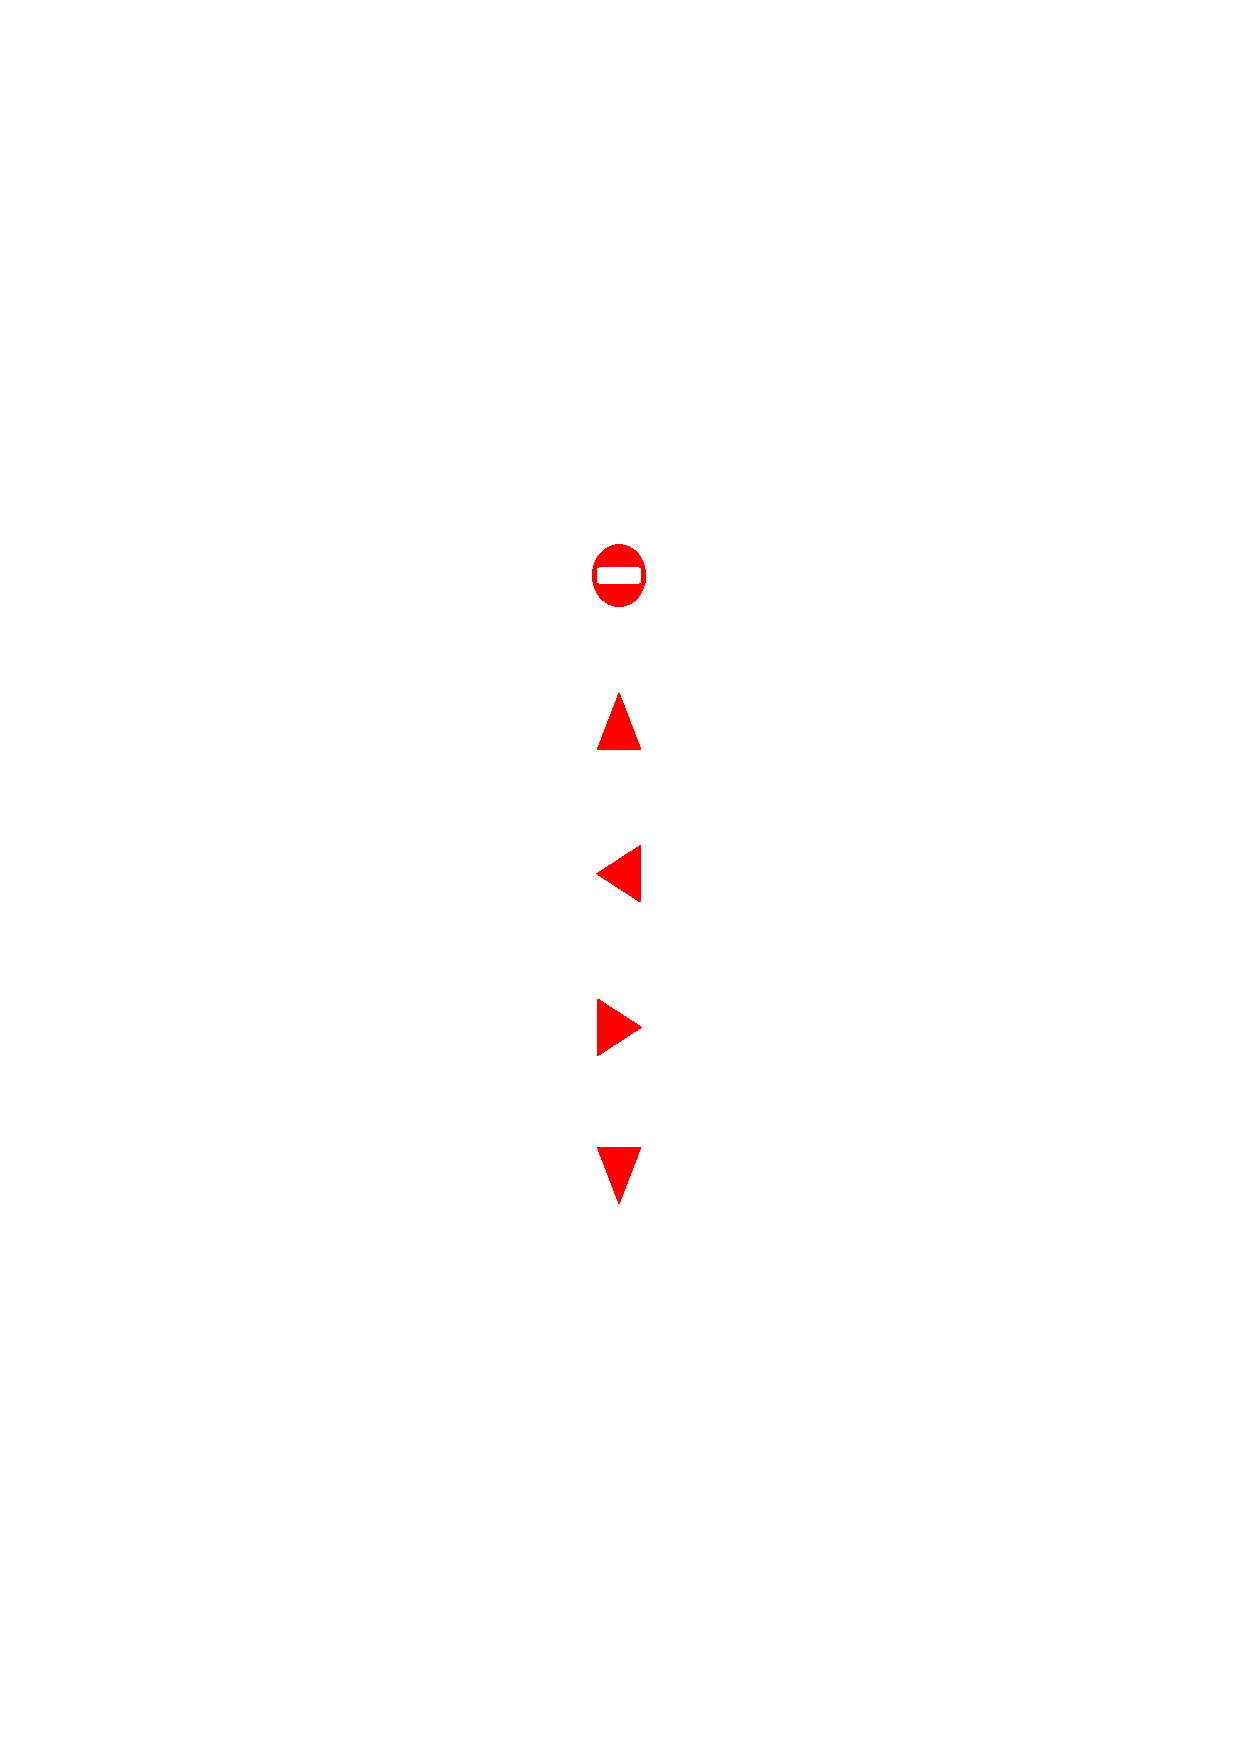
\includegraphics[scale=.5,trim=9.1cm 16cm 9.5cm 10.5cm,clip]{signs.pdf}\end{minipage}	& 0 1 1 1 0	& 14 & Move straight forward (follow the track to the forward direction) \\ \hline
		\begin{minipage}{.075\textwidth}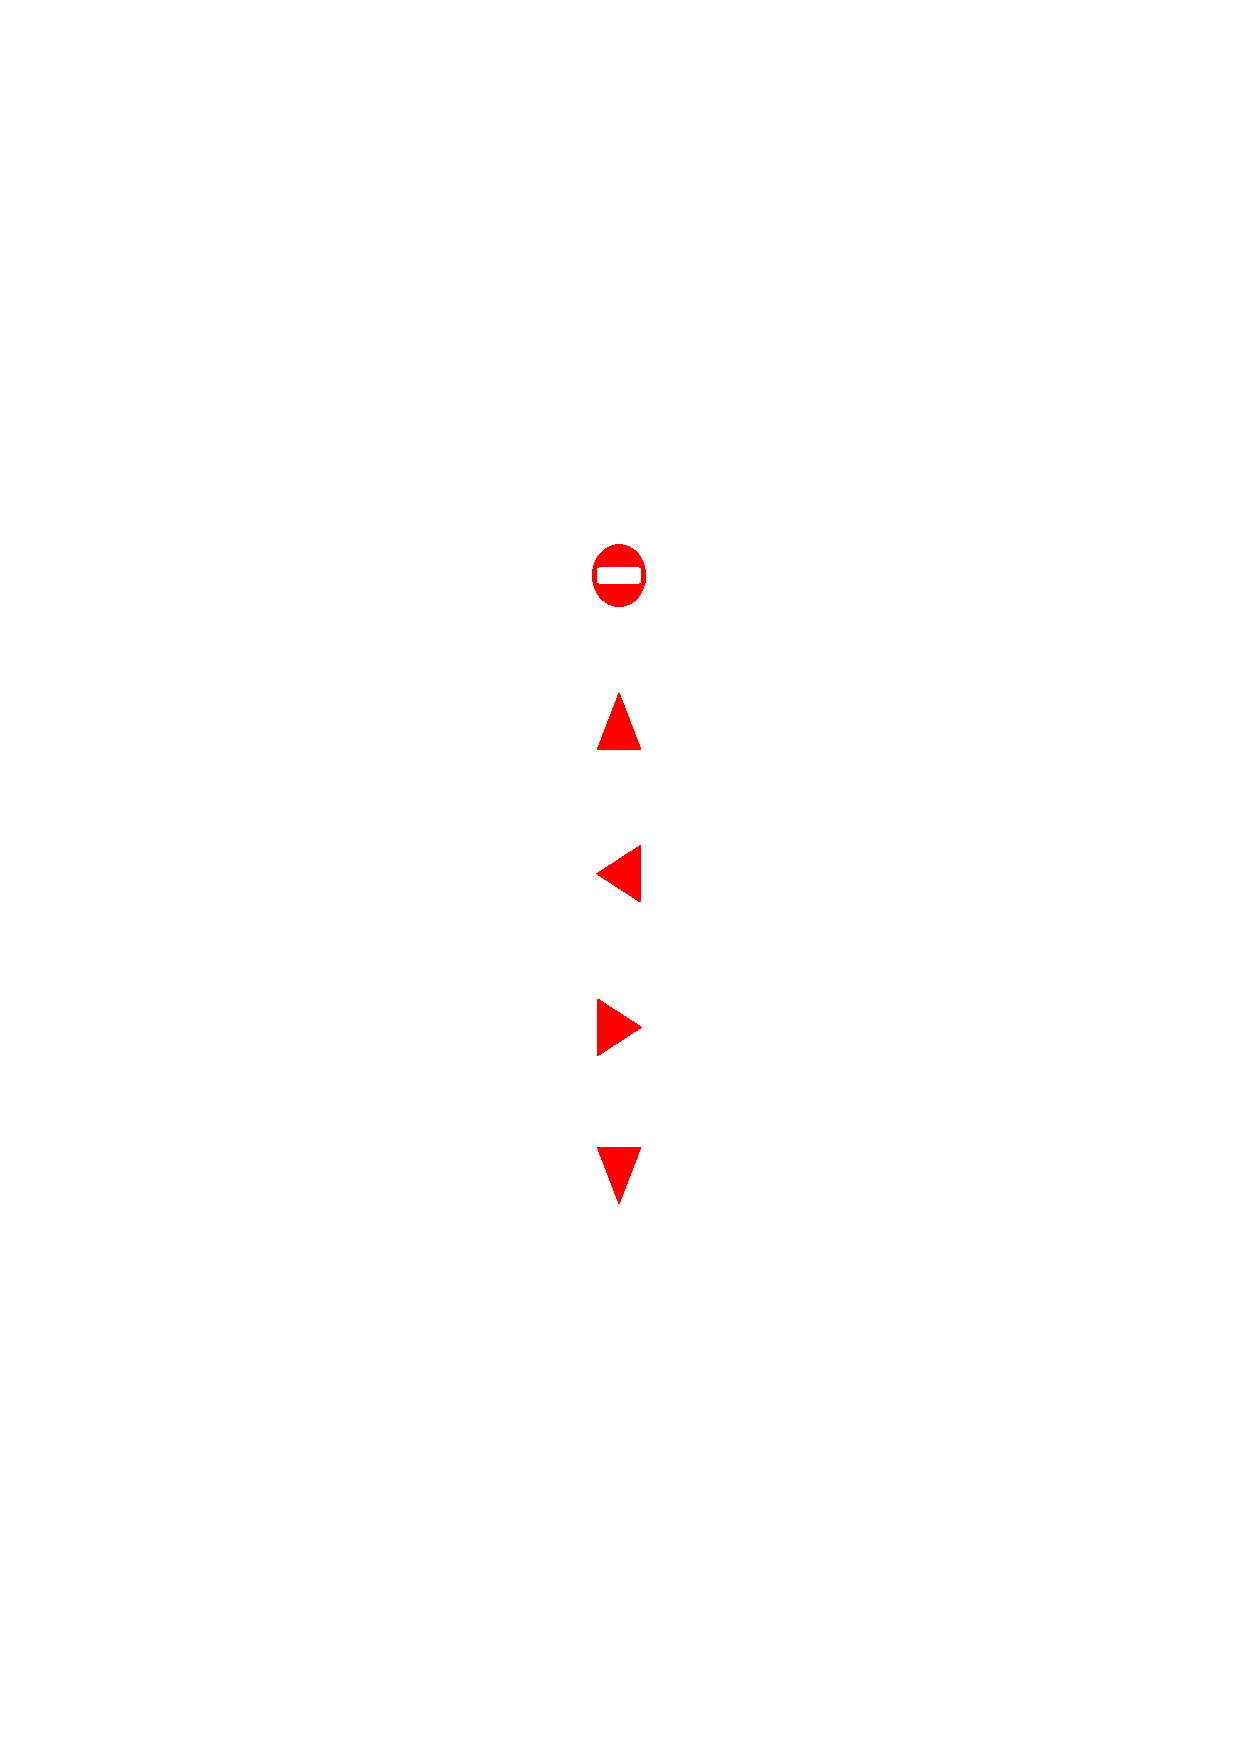
\includegraphics[scale=.5,trim=9.1cm 13.5cm 9.5cm 13cm,clip]{signs.pdf}\end{minipage}		& 1 1 1 0 0 & 28 & Move to the left (follow the track to the left direction) \\ \hline
		\begin{minipage}{.075\textwidth}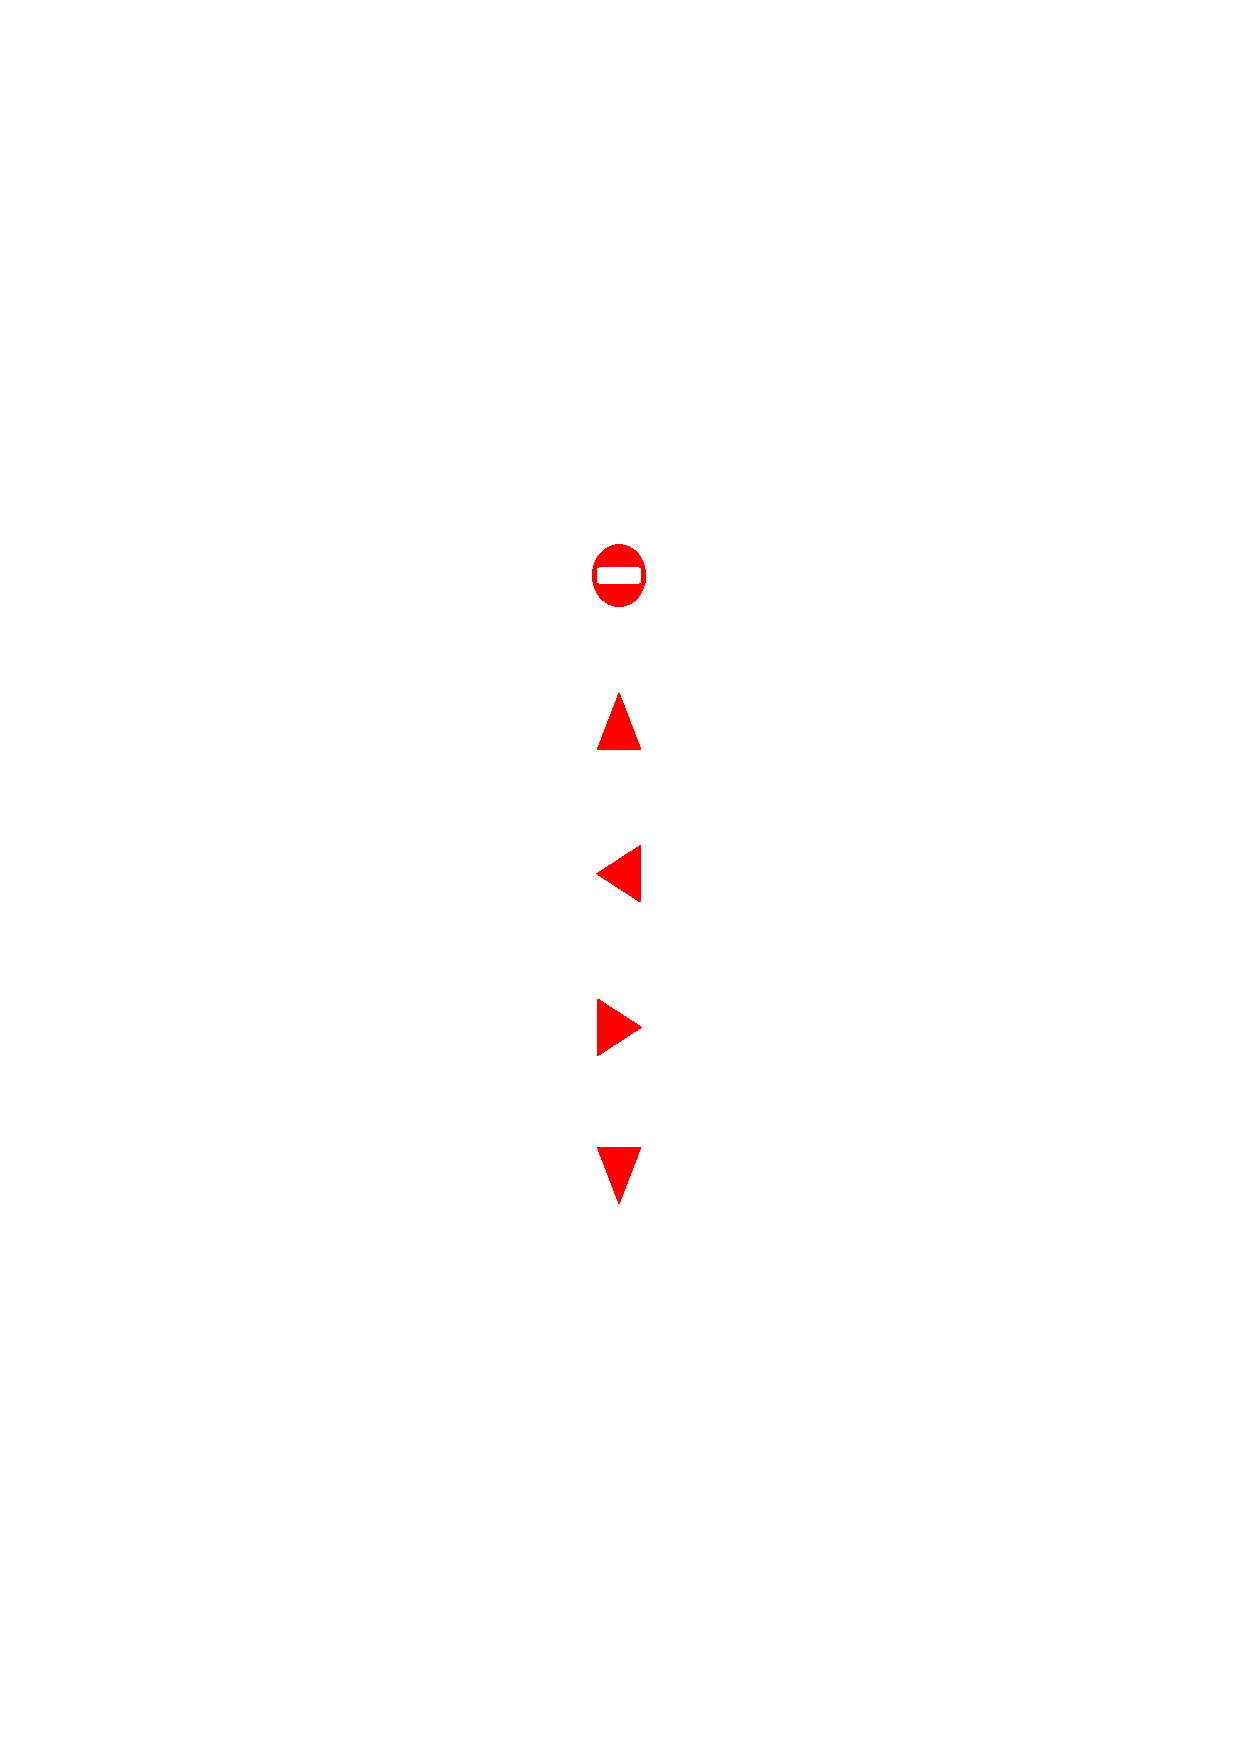
\includegraphics[scale=.5,trim=9.1cm 10.75cm 9.5cm 15.75cm,clip]{signs.pdf}\end{minipage}	& 0 0 1 1 1 & 7 & Move to the right (follow the track to the right direction) \\ \hline
		\begin{minipage}{.075\textwidth}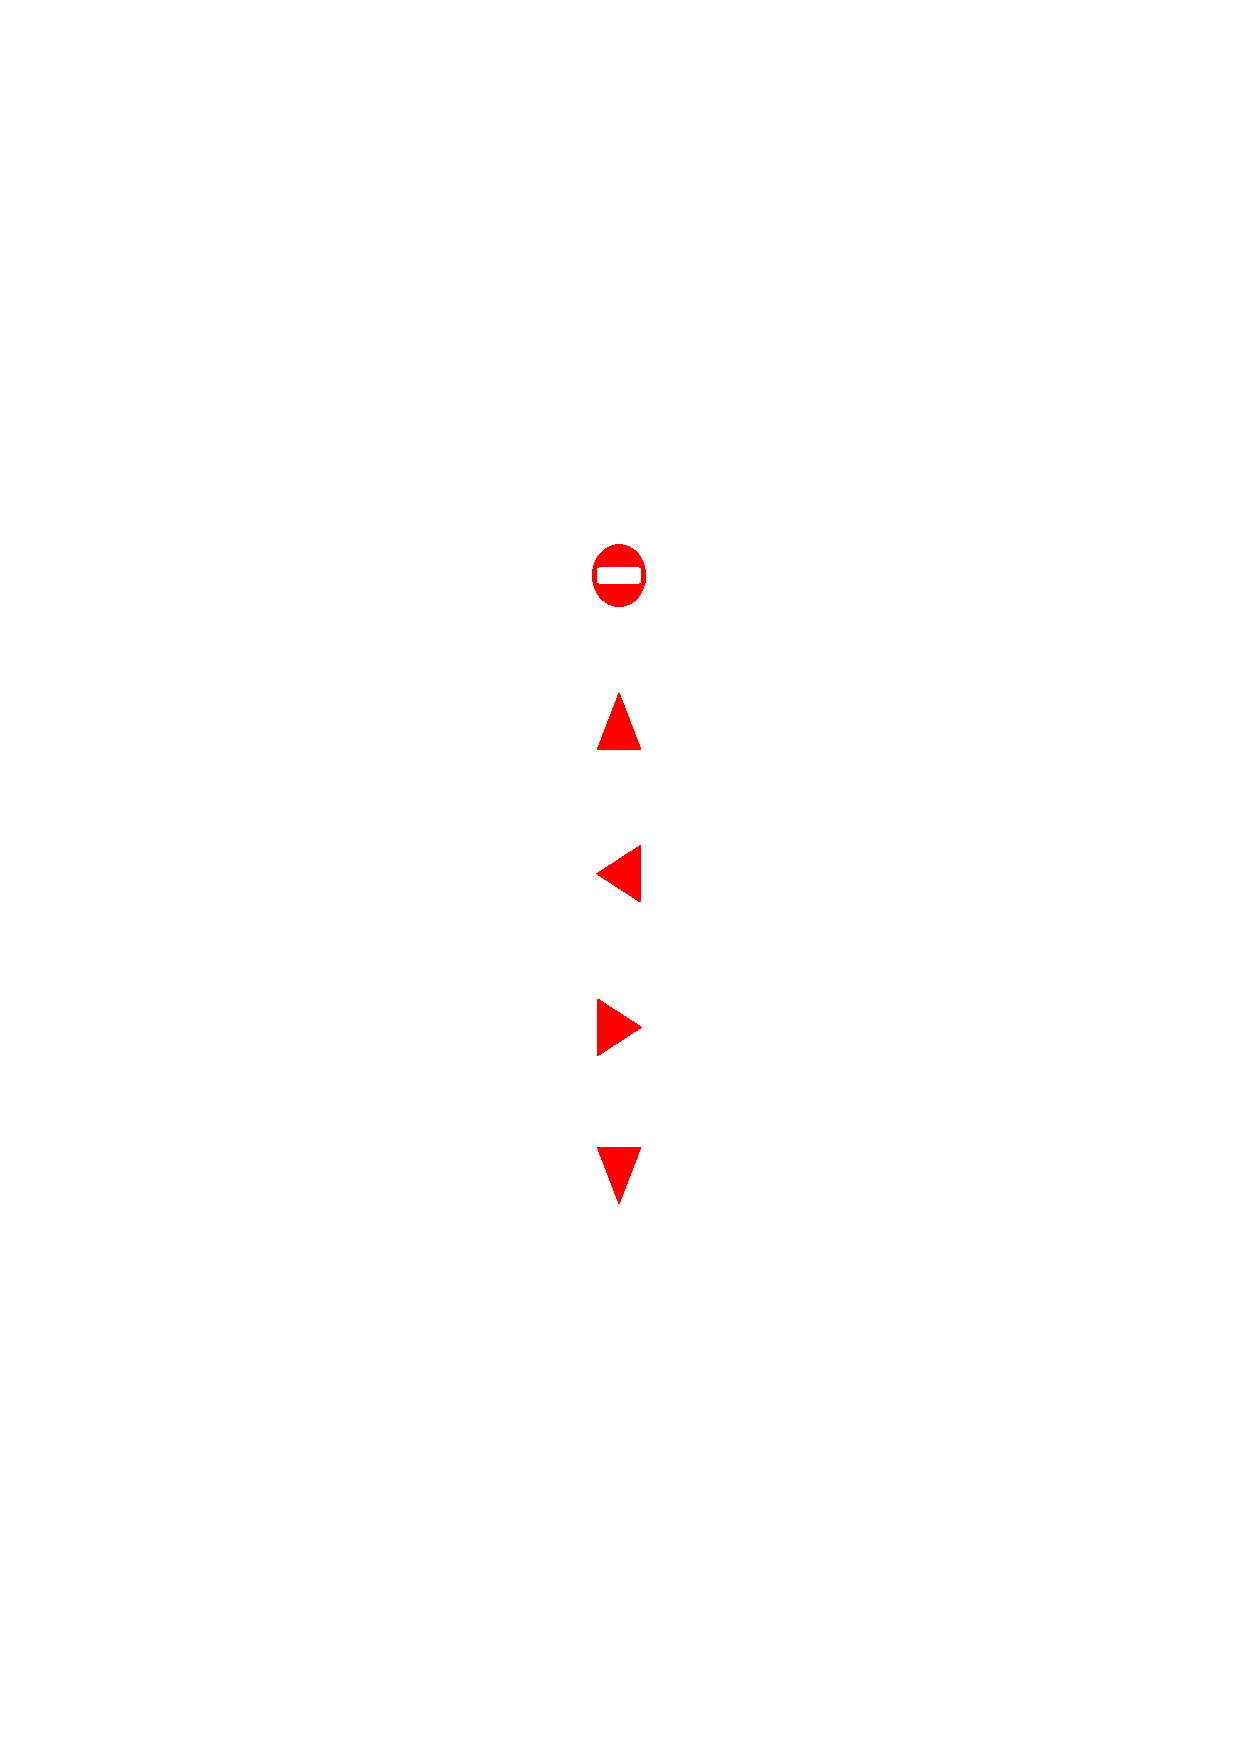
\includegraphics[scale=.5,trim=9.1cm 8.5cm 9.5cm 18cm,clip]{signs.pdf}\end{minipage} & 1 1 1 1 1 & -31 & Move backward (reverse moving to the back) \\ \hline
	\end{tabular}
\end{table}

\subsection{Policy search:} 
Principally, there are two essential types of reinforcement learning methods - policy search and value function. The first type refers to methods that consider searching for the optimal policy $\pi^*$. The second type refers to methods that consider investigating the optimal value-state function $V^*(s)$ \cite{Arulkumaran2017Deep}. In this work, the suggested DRL-RT network is based on the policy search. According to the MDP concept, the DRL-RT collects input images as current states $S_t$ and getting advantages from rewards $R$ to generate actions $A$, then the actions predict new states $S_{t+1}$. Consequently, the new states can be transitioned again in the inputs as current states. 

The essential equation of the policy search is demonstrated as:
\begin{equation}
\pi^*=\underset{\pi}{argmax}~\mathbb{E} [R\mid\pi]
\label{Eq:MDP}
\end{equation}
where $\pi$ is the policy and $\mathbb{E}$ is the expected return value \cite{arulkumaran2017brief}. In this work, the reward $R$ of the correct tracking is considered as (+1), whereas, the reward $R$ of the incorrect tracking is considered as (-1). Measuring the successful process of the road tracking will be based on obtaining as many positive rewards as possible. 

\subsection{Proposed DRL-RT:} 
An applicable deep reinforcement network named the DRL-RT is established for road tracking. It consists of eight layers: two convention layers, two Rectified Linear Unit (ReLU) layers, a pooling layer, a fully connected layer, a regression layer and a classification layer. The input is an image of a car facing view, and it is considered as a current state. The input image size has been reduced to $254 \times 427 \times 3$ pixels in order to speed up the deep learning processes. The first layer after the input is a convolution layer, it consists of 5 filters each of which has a filter size of $10 \times 10$ pixels. This layer is important to extract the main features of the input images. A ReLU layer is used in the second layer. It removes the negative values and maintain the positive values of the previous layer. The third layer is also a convolution layer, it consists of 5 filters each of which has a filter size of $5 \times 5$ pixels. It extracts more features from the input images. A ReLU layer is employed again in the fourth layer. This layer rectifies the negative values. It has empirically been found that using two convolution layers with two ReLU layers can well analyse the information before being compressed by applying the next layer. Then, a pooling layer of a maximum type is applied in the fifth layer, the filter size here is $3 \times 3$ pixels with a stride of 3 pixels. The sixth layer is a fully connected layer, it collects the outputs from the previous layer and produces a series of decimal code tracking values. A regression layer is the seventh layer. In this layer, a series of directional road tracking codes are generated. The successful codes in this layer produce positive rewards, whereas, unsuccessful codes generate negative rewards. The network should be propagated, forwarded and backwarded the information for updating the network weights, during the training stage till obtaining as many positive rewards as possible. Given the codes in the regression layer, it is the classification layer's task to generate a new action - one of the five as in Table \ref{Table:Signs_codes}. Fig. \ref{Fig:Deep_Reinf_Net} shows the proposed DRL-RT network.

\subsection{Theoretical concepts:} 
The theoretical concepts of the main analysis layers (convolution, ReLU, pooling and fully connected) in the DRL-RT network were stated in \cite{omar2018deep}.

In the first and third layers, the collected information will be converted to feature maps. The feature map is defined as a convoluted 2D image with a kernel of weights. The following general equation represents the operations in a convolution layer:
\begin{equation}
z_{u,v,c^{l}}= \text{\footnotesize $B_{c^{l}}+\sum_{i=-k_h^{l}}^{k_h^{l}}\sum_{j=-k_w^{l}}^{k_w^{l}}\sum_{c^{l-1}=1}^{C^{l-1}} W_{i+k_h^{l},j+k_w^{l},c^{l-1}}^{c^{l}} z_{u+i,v+j,c^{l-1}}$}
\label{eq:conv_layer}
\end{equation}
where $z_{u,v,c^{l}}$ is a convolution layer outcome, $(u,v)$ is the assigned pixel, $c^{l}$ is the channel number of the convolution layer,  $W_{i,j,c^{l-1}}^{c^{l}}$ is the components of the kernel weights,  $B_{c^{l}}$ is the channel bias of the convolution layer, $k_h^l$ and $k_w^l$ are respectively the height and width of the kernel weights of the convolution layer, $C$ is the number of channels and it is here equal to 3 as we are using three channels of coloured images, $l-1$ is the previous layer, and $l$ is the current layer (the convolution layer) \cite{simo2016learning}. 
% \marginpar{Does it mean that all the $k_w^l$ are the same for all layers?}. Answer is: no and I have mentioned previously that $l$ represents the current layer.
%Again, this layer analyses the input values and produces FTs' feature maps.

A ReLU transfer function is applied in the second and fourth layers. This function can provide non-linear calculation to the DRL-RT. The ReLU function maintains the positive values and discards the negative values of a previous layer. Equation \eqref{eq:relu_layer} is exploited for the ReLU transfer function:
\begin{equation}
o_{u,v,c^{l}}=f(z_{u,v,c^{l}})=\max(0,z_{u,v,c^{l}})
\label{eq:relu_layer}
\end{equation}
where $o_{u,v,c^{l}}$ is a ReLU layer outcome and $\max$ is the maximum operation \cite{krizhevsky2012imagenet}. 

A pooling layer is used in the fifth part of the DRL-RT. The pooling layer can reduce the sizes of the feature maps. It obtains the maximum values from the last ReLU layer. In general, the pooling layer can be applied according to the following equation:
\begin{equation}
q_{a^{l},b^{l},c}=\underset{0\leq a<p_h,0\leq b<p_w}{\max} o_{a^{l}\times p_h+a,~b^{l}\times p_w+b,~c}
\label{eq:pooling_layer}
\end{equation}
where $q_{a^{l},b^{l},c}$ is a pooling layer outcome, $0\leq a^{l} <p_h^{l}$, $p_h^{l}$ is the height of the resulting feature maps, $0\leq b^{l} <p_w^{l}$, $p_w^{l}$ is the width of the resulting feature maps, $0\leq c <C^{l}=C^{l-1}$, $p_h$ and $p_w$ are respectively the width and height of the feature map sub-areas that require pooling \cite{wu2017introduction}. 

Subsequently, the fully connected layer is used to match between the designed number of subjects and the data of the pooling layer. Equation (\ref{eq:fully_connect}) demonstrates the fully connected layer processes:
\begin{equation}
g_{r}=\text{\footnotesize $\sum_{a=1}^{m_1^{l-1}} \sum_{b=1}^{m_2^{l-1}} \sum_{c=1}^{m_3^{l-1}} W_{a,b,c,r}^{l}(\textit{\textbf{Q}}_{c})_{a,b}~, ~~~~~~~\forall 1 \leq r \leq m^{l}$}
\label{eq:fully_connect}
\end{equation}
where $g_{r}$ is a fully connected layer outcome, $m_1^{l-1}$ and $m_2^{l-1}$ are the width and height of a feature map in the previous layer (the pooling layer) respectively, $m_3^{l-1}$ is the number of produced feature maps in the pooling layer, $W_{a,b,c,r}^{l}$ is the connection weights between the fully connected layer and the pooling layer, $\textit{\textbf{Q}}_{c}$ are the pooling layer outputs, and $m^{l}$ is the number of designed subjects \cite{stutz2014neural}.

The computations of the regression layer in the suggested DRL-RT network are based on the Mean Squared Error (MSE). The main MSE equation is illustrated as:
\begin{equation}
MSE=\frac{1}{n} \sum_{r=1}^{n}(t_r-g_r)^2
\label{eq:fully_connect}
\end{equation}
where $n$ is the number of computed values and $t$ is the desired output values \cite{saugirouglu2009intelligent}. If the regression output values close to the desired code values, positive rewards are produced. Otherwise, negative rewards are generated. 

Finally, the classification layer translates the regression information into actions by converting the obtained values into their assigned classes.

The MDP has been applied to the DRL-RT by providing current road tracking as current states $S_t$ to the input layer, estimating tracking directions as actions $A$, considering correct and incorrect tracking actions as rewards $R$, and predicting next tracking movements as new states $S_{t+1}$. Then, the new state (or next tracking view) are transitioned as a current state to the DRL-RT input layer in order to produce a new state again.
\begin{table*}[!t]
	\centering
	\caption{Examples of the four employed environments}
	\label{Table:Environments_Examples}
	\begin{tabular}{|C{1cm}|c|C{13.5cm}|}
		\hline
		\textbf{Database no.} & \textbf{Environment} & \textbf{Examples} \\ \hline
		(1)	& Spring & \begin{minipage}{.9\textwidth}\includegraphics[scale=.8,trim=2cm 24.5cm 2cm 2.5cm,clip]{examples.pdf}\end{minipage} \\ \hline
		%			&&\\ \hline
		(2) & Fog	& \begin{minipage}{.9\textwidth}\includegraphics[scale=.8,trim=2cm 20.5cm 2cm 6.5cm,clip]{examples.pdf}\end{minipage} \\ \hline
		%			&&\\ \hline
		(3)	& Rain &  \begin{minipage}{.9\textwidth}\includegraphics[scale=.8,trim=2cm 16.5cm 2cm 10.5cm,clip]{examples.pdf}\end{minipage} \\ \hline
		%			&&\\ \hline
		(4)	& Heavy- rain & \begin{minipage}{.9\textwidth}\includegraphics[scale=.8,trim=2cm 12.5cm 2cm 14.3cm,clip]{examples.pdf}\end{minipage} \\ \hline
		%			&&\\ \hline
	\end{tabular}
\end{table*}

%%%%%%%%%%%%%%%%%%%%%%%%%%%%%%%%%%%%%%%%%%%%%%%%%%%%%%%%%%%%%%%%
% Contents: Math typesetting with LaTeX
% $Id$
%
% Changes by Stefan M. Moser: 2008/10/22
%
% -Section 2: "Single Equations": added comment about preference of
%  equation* over \[
% -Replaced (almost) all examples with \[ by equation*
% -New section 4: "Single Equations that are Too Long: multline"
% -New section 5: "Multiple Equations"
% -Section 6: "Arrays and Matrices": made a full section and added
%  some material
% -Section 9: "Theorems, Lemmas, ...": added a subsection about proofs
%  with new material
%
% Other Changes:
% -in lshort.sty: 
%    *example environment adapted: changed in three places
%     \textwidth by \linewidth. This is necessary for
%     example-environment within a itemize-list.
%    *added \RequirePackage[retainorgcmds]{IEEEtrantools}
%
% THINGS TO DO:
% -adapt typesetting of new sections to rest of lshort, including all
%  the usual commands used so far. In particular, I guess we have to
%  get rid of the \verb-commands everywhere
% -include index-commands
%%%%%%%%%%%%%%%%%%%%%%%%%%%%%%%%%%%%%%%%%%%%%%%%%%%%%%%%%%%%%%%%%
 
\chapter{Results}

\section{Results}
\subsection{Databases:} 
Four databases from SYNTHIA \cite{Ros2016TheSYNTHIA} are used. The selected databases are constructed under different environment conditions: (1) spring, (2) fog, (3) rain and (4) heavy-rain. Moreover, their segmented images, which are provided by the same database, are found to be useful for manually determining the appropriate code of each track. Examples from the four databases are given in Table \ref{Table:Environments_Examples}.	

All implementations were performed by employing a computer with the following facilities: 8 GB RAM and Intel Core i5 processor (3.2 GHz). Only the microprocessor was used in this study to train and test the DRL-RT. The number of frames that have been utilized here are: 270, 284, 268 and 248 frames for the environments of spring, fog, rain and heavy-rain, respectively. The frames are equally divided between the training and testing stages (50\% each), where the odd frames are used in the training stage and the even frames are used in the testing stage.

\begin{figure}[!t]
	\centering
	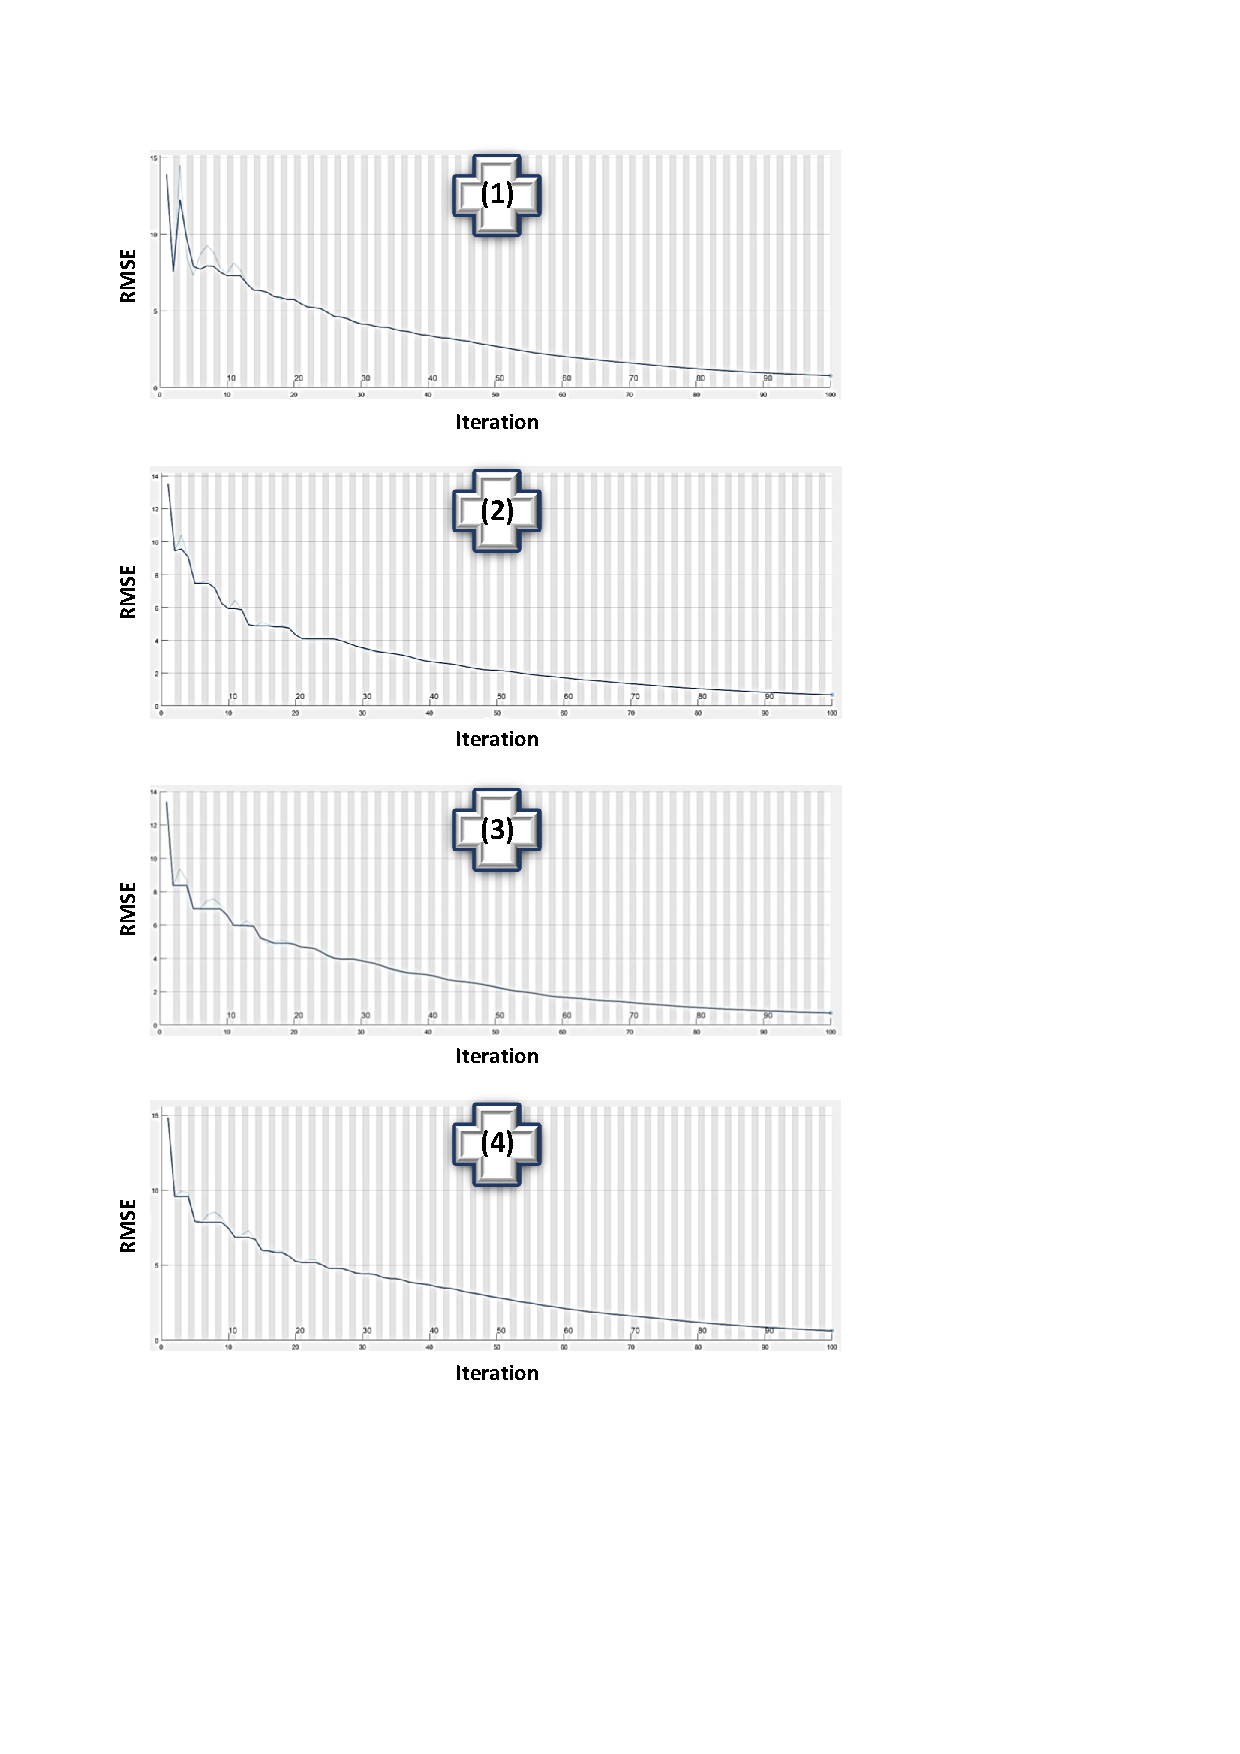
\includegraphics[scale=.67,trim=2cm 6cm 6.5cm 2cm,clip]{training_curves.pdf}
	\caption{The training performance of the DRL-RT for the: (1) spring environment, (2) fog environment, (3) rain environment and (4) heavy-rain environment}
	\label{fig:training_curves}
\end{figure}

\subsection{Training stage:} 
The suggested DRL-RT network has been separately trained for each environment. The following parameters have been assigned for the trainings: Adaptive Moment Estimation (ADAM) optimizer \cite{kingma2014adam}, learning rate equal to 0.0003, gradient decay factor ($\beta_1$) equal to 0.9, squared gradient decay factor ($\beta_2$) equal to 0.99 and mini batch size equal to 128. The training performance of the DRL-RT for the four databases are given in Fig. \ref{fig:training_curves}. This figure demonstrates the relationships between the Root Mean Square Error (RMSE) and the training iterations during the training stages. The RMSE values are usually exploited to demonstrate the differences between desired values and output values.	These differences are usually reduced during the proceeding of training itrations. Clearly, the curves are successfully declined toward goals.

\subsection{Testing stage:} 
The results of the testing stages are interested as it can be observed in Fig. \ref{fig:Main_Results}. To illustrate, the driving accuracy attained its highest value of 93.94\% by using the spring environment database. This is because that the DRL-RT has analysed very clear provided images.  The fog environment database obtained a high driving accuracy of 93.66\%. Here, the overall views are blurred but the road tracking can still be distinguished. The DRL-RT could recognize the road tracking but with slightly lower accuracy than the spring views. The driving accuracy of the rain environment database achieved 89.55\% and this is due to the noise effects of rain drops on image views. Finally, the inferior driving accuracy of 84.68\% was recorded for the heavy-rain environment database as the amount of rain drops (or noise) are increased here.
\begin{figure}[!t]
	\centering
	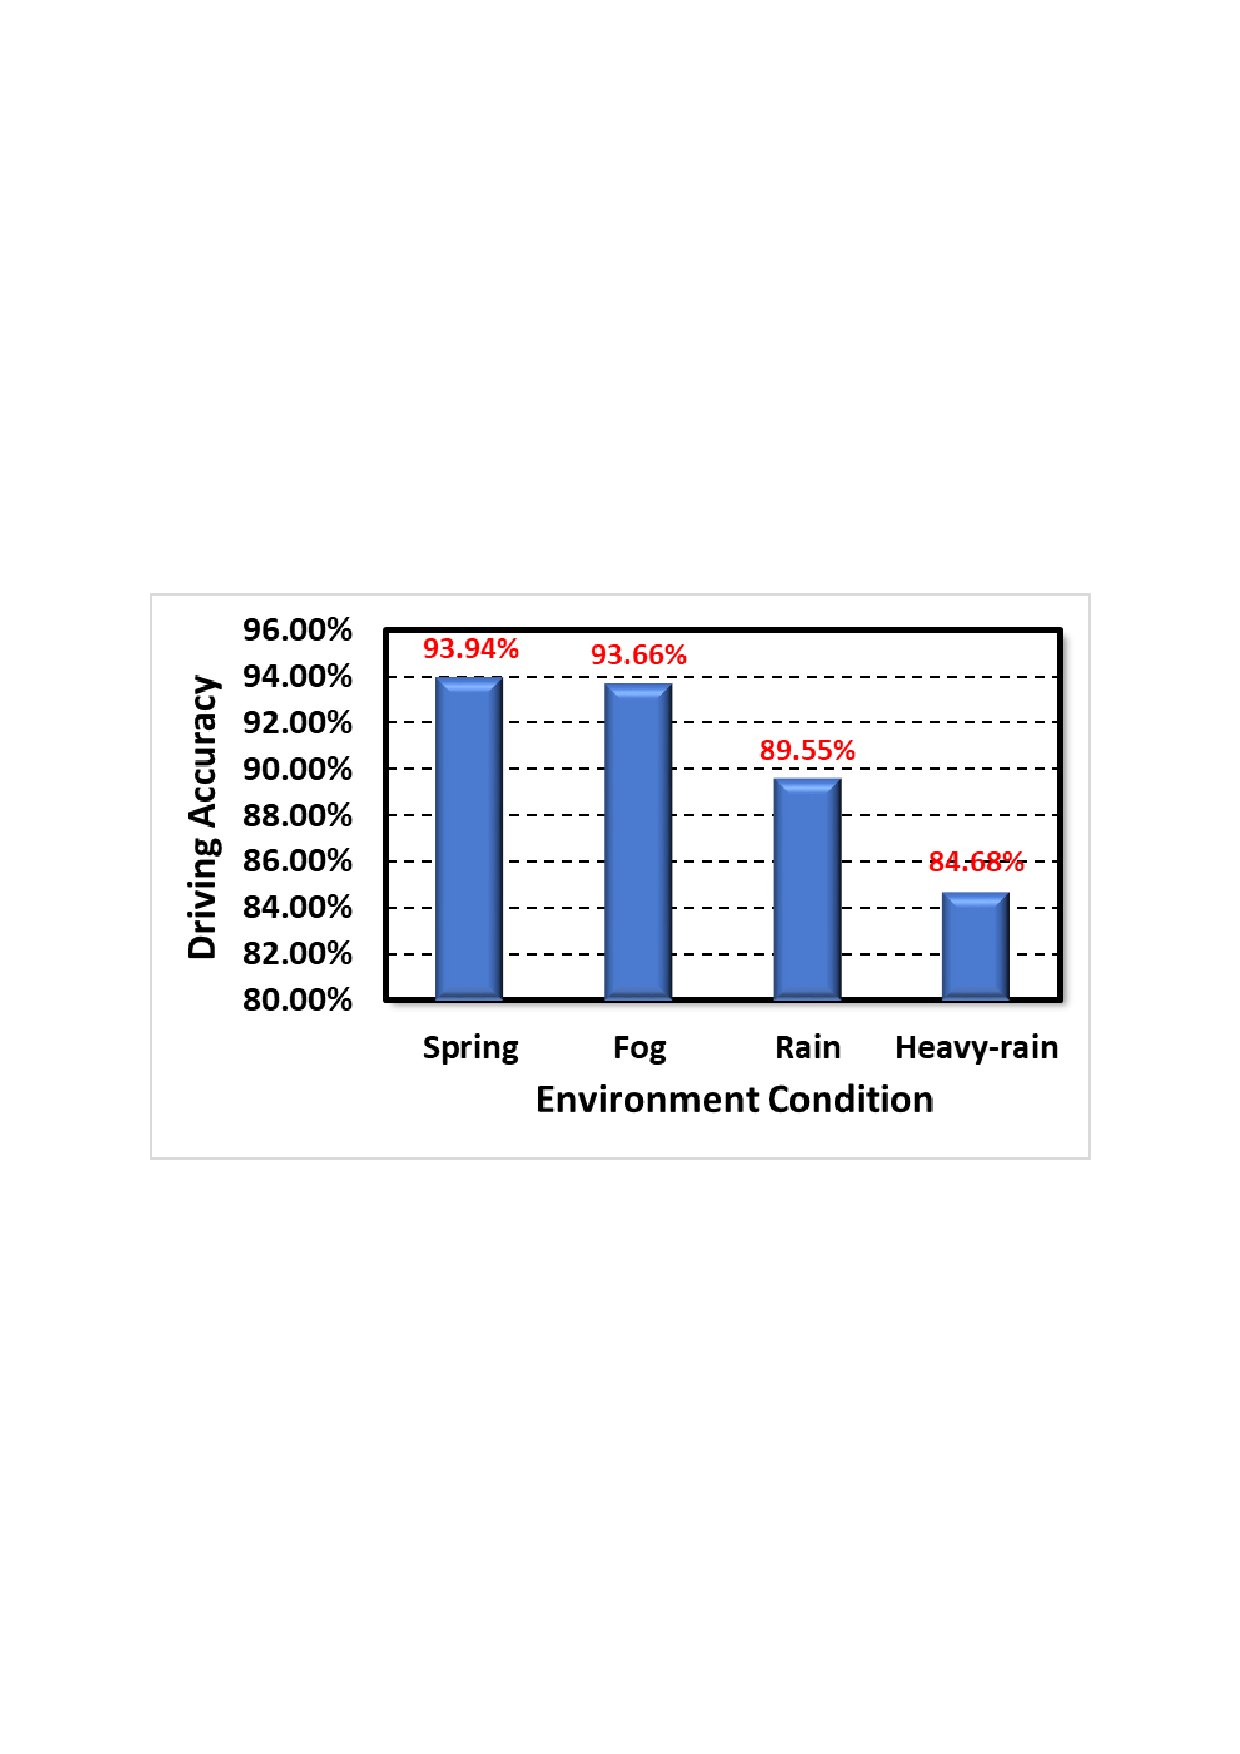
\includegraphics[scale=.58,trim=3cm 10.3cm 2.7cm 10.3cm,clip]{Main_Results.pdf}
	\caption{The performance of the DRL-RT under different employed environments}
	\label{fig:Main_Results}
\end{figure}

\subsection{Comparisons:} 
In the case of comparisons, hard efforts were performed to investigate and simulate various deep learning approaches. Comparisons have been established between our proposed DRL-RT method and other suggested networks. Table \ref{Table:Comparisons} shows the accuracies of different deep learning networks by applying the database of SYNTHIA-SEQS-05-SPRING, some parameters were reasonably changed to allow acceptable comparisons. The reason of selecting this database here is that it has the clear environment, which is suitable to discard undesired effects and provide fair judgement.

\begin{table}[]
	\centering
	\caption{A comparison between our proposed DRL-RT method and other suggested networks}
	\label{Table:Comparisons}
	\begin{tabular}{|C{3cm}|c|c|}
		\hline
		\textbf{Reference} & \textbf{Deep learning method} & \textbf{Accuracy} \\ \hline
		Karaduman and Eren \cite{Karaduman2017Deep} & CNN & 67.42\% \\ \hline
		Bojarski \textit{et al.} \cite{bojarski2016end} & CNN & 74.24\% \\ \hline
		George and Routray \cite{George2016Real} & CNN & 83.33\% \\ \hline
		Yun \textit{et al.} \cite{Yun2017Action,Yun2018Action} & ADNet & 83.33\% \\ \hline
		Mnih \textit{et al.} \cite{mnih2015human} & DQN & 88.64\% \\ \hline
		Proposed method & DRL-RT & 93.94\% \\ \hline
	\end{tabular}
\end{table}

From Table \ref{Table:Comparisons}, it can be seen that the suggested CNN in \cite{Karaduman2017Deep} obtained the inferior tracking accuracy of 67.42\%. This is due to the architecture of this network, where it constructed to classify directions of traffic signs. More specifically, a pooling layer was applied after each convolution layer and no ReLU layers were used. This caused compressing and wasting useful extracted features after each convolution layer. The CNN which is used in \cite{bojarski2016end} attained a low accuracy of 74.24\%. The main drawback of this network is that it considers steering angles to be tracked, where this increases the erroneous of obtaining precise outputs. The CNN in \cite{George2016Real} achieved 83.33\%. This is also due to the architecture of this network, which was designed for classifying eye gaze directions. The ADNet which was approached in \cite{Yun2017Action,Yun2018Action} attained the same accuracy of 83.33\%. 
%	The architecture of this network was mainly consists of convolution layers and fully connected layers, this seems not 
The essential problem here is represented by the considered rewards, which were basically designed %after moving objects and not during the moving. 
for recognizing moved objects as the rewards are updated in the stop action. In addition, the Adnet architecture is not so appropriate for road tracking tasks. The Deep Q-Network (DQN), which is proposed in \cite{mnih2015human} and illustrated in \cite{arulkumaran2017brief} achieved reasonable accuracy of 88.64\%. This can be due to the DQN processes, where it combines between the deep network and the Q-learning. This network can be considered as the nearest method to our approach. Finally, our proposed method has shown superior performance by attaining the accuracy of 93.94\%. This can be due to the overall structure of our road tracking method including the network architecture, tracking policy and designed codes. 
%%%%%%%%%%%%%%%%%%%%%%%%%%%%%%%%%%%%%%%%%%%%%%%%%%%%%%%%%%%%%%%%%
% Contents: TeX and LaTeX and AMS symbols for Maths
% $Id$
%%%%%%%%%%%%%%%%%%%%%%%%%%%%%%%%%%%%%%%%%%%%%%%%%%%%%%%%%%%%%%%%%


\chapter{Conclusion}  \label{symbols}

\section{Conclusion}
A deep reinforcement neural network is established for road tracking termed the DRL-RT. This network is suggested to guide driving cars under different weather environments. Different tracking instances were coded to represent the appropriate road tracking. The MDP concept is used here, where the network accepted states and produced actions by taking advantages from rewards. The proposed deep reinforcement network is based on the policy search. This study were compared with other work and it reported superior performance. In addition, interesting results were benchmarked by the proposed approach. That is, the best performance of 93.94\% was recorded for a clear environment and reasonable performance were reported under unclear environments of fog, rain and heavy-rain as the obtained accuracies were respectively equal to 93.66\%, 89.55\% and 84.68\%. 

%%%%%%%%%%%%%%%%%%%%%%%%%%%%%%%%%%%%%%%%%%%%%%%%%%%%%%%%%%%%%%%%%%
% Contents: Specialities of the LaTeX system
% $Id$
%%%%%%%%%%%%%%%%%%%%%%%%%%%%%%%%%%%%%%%%%%%%%%%%%%%%%%%%%%%%%%%%%

\chapter{Specialities}
\begin{intro}
  When putting together a large document, \LaTeX{} will help
  with some special features like index generation,
  bibliography management, and other things.
  A much more complete description of specialities and
  enhancements possible with \LaTeX{} can be found in the
  {\normalfont\manual{}} and {\normalfont \companion}.
\end{intro}


\section{Bibliography}

Produce a \wi{bibliography} with the \ei{thebibliography}
environment.  Each entry starts with
\begin{lscommand}
\ci{bibitem}\verb|[|\emph{label}\verb|]{|\emph{marker}\verb|}|
\end{lscommand}
The \emph{marker} is then used to cite the book, article or paper
within the document.
\begin{lscommand}
\ci{cite}\verb|{|\emph{marker}\verb|}|
\end{lscommand}
If you do not use the \emph{label} option, the entries will get enumerated
automatically.  The parameter after the \verb|\begin{thebibliography}|
command defines how much space to reserve for the number of labels. In the example below,
\verb|{99}| tells \LaTeX{} to expect that none of the bibliography item numbers will be wider
than the number 99.
\enlargethispage{2cm}
\begin{example}
Partl~\cite{pa} has
proposed that \ldots
\begin{thebibliography}{99}
\bibitem{pa} H.~Partl:
\emph{German \TeX},
TUGboat Volume~9, Issue~1 (1988)
\end{thebibliography}
\end{example}

\chaptermark{Specialities} % w need to fix the damage done by the
                           %bibliography example.
\thispagestyle{fancyplain}


For larger projects, you might want to check out the Bib\TeX{}
program. Bib\TeX{} is included with most \TeX{} distributions. It
allows you to maintain a bibliographic database and then extract the
references relevant to things you cited in your paper. The visual
presentation of Bib\TeX{}-generated bibliographies is based on a style-sheets concept that allows you to create bibliographies following
a wide range of established designs.

\section{Indexing} \label{sec:indexing}
A very useful feature of many books is their \wi{index}. With \LaTeX{}
and the support program \texttt{makeindex},\footnote{On systems not
  necessarily supporting
  filenames longer than 8~characters, the program may be called
  \texttt{makeidx}.} an index can be generated quite easily.  This
introduction will only explain the basic index generation commands.
For a more in-depth view, please refer to \companion.  \index{makeindex
  program} \index{makeidx package}

To enable their indexing feature of \LaTeX{}, the \pai{makeidx} package
must be loaded in the preamble with
\begin{lscommand}
\verb|\usepackage{makeidx}|
\end{lscommand}
\noindent and the special indexing commands must be enabled by putting
the
\begin{lscommand}
  \ci{makeindex}
\end{lscommand}
\noindent command in the preamble.

The content of the index is specified with
\begin{lscommand}
  \ci{index}\verb|{|\emph{key}@\emph{formatted\_entry}\verb|}|
\end{lscommand}
\noindent commands, where \emph{formatted\_entry} will appear in the index
and \emph{key} will be used for sorting.  The \emph{formatted\_entry} is
optional. If it is missing the \emph{key} will be used. You enter the index
commands at the points in the text that you want the final index entries to
point to.  Table~\ref{index} explains the syntax with several examples.

\begin{table}[!tp]
\caption{Index Key Syntax Examples.}
\label{index}
\begin{center}
\begin{tabular}{@{}lll@{}}
  \textbf{Example} &\textbf{Index Entry} &\textbf{Comment}\\\hline
  \rule{0pt}{1.05em}\verb|\index{hello}| &hello, 1 &Plain entry\\
\verb|\index{hello!Peter}|   &\hspace*{2ex}Peter, 3 &Subentry under `hello'\\
\verb|\index{Sam@\textsl{Sam}}|     &\textsl{Sam}, 2& Formatted entry\\
\verb|\index{Lin@\textbf{Lin}}|     &\textbf{Lin}, 7& Formatted entry\\
\verb|\index{Kaese@K\"ase}|     &\textbf{K\"ase}, 33& Formatted entry\\
\verb.\index{ecole@\'ecole}.     &\'ecole, 4& Formatted entry\\
\verb.\index{Jenny|textbf}.     &Jenny, \textbf{3}& Formatted page number\\
\verb.\index{Joe|textit}.     &Joe, \textit{5}& Formatted page number
\end{tabular}
\end{center}
\end{table}

When the input file is processed with \LaTeX{}, each \verb|\index|
command writes an appropriate index entry, together with the current
page number, to a special file. The file has the same name as the
\LaTeX{} input file, but a different extension (\verb|.idx|). This
\eei{.idx} file can then be processed with the \texttt{makeindex}
program:

\begin{lscommand}
  \texttt{makeindex} \emph{filename}
\end{lscommand}
The \texttt{makeindex} program generates a sorted index with the same base
file name, but this time with the extension \eei{.ind}. If now the
\LaTeX{} input file is processed again, this sorted index gets
included into the document at the point where \LaTeX{} finds
\begin{lscommand}
  \ci{printindex}
\end{lscommand}

The \pai{showidx} package that comes with \LaTeXe{} prints out all
index entries in the left margin of the text. This is quite useful for
proofreading a document and verifying the index.

Note that the \ci{index} command can affect your layout if not used carefully.

\begin{example}
My Word \index{Word}. As opposed
to Word\index{Word}. Note the
position of the full stop.
\end{example}

\texttt{makeindex} has no clue about characters outside the ASCII range. To
get the sorting correct, use the \verb|@| character as shown in the K\"ase
and \'ecole examples above.

\section{Fancy Headers}
\label{sec:fancy}

The \pai{fancyhdr} package,\footnote{Available from
  \CTAN|macros/latex/contrib/supported/fancyhdr|.} written by
Piet van Oostrum, provides a few simple commands that allow you to
customize the header and footer lines of your document.  Look
at the top of this page, for an application of this
package.

\begin{figure}[!htbp]
\begin{lined}{\textwidth}
\begin{verbatim}
\documentclass{book}
\usepackage{fancyhdr}
\pagestyle{fancy}
% with this we ensure that the chapter and section
% headings are in lowercase.
\renewcommand{\chaptermark}[1]{%
        \markboth{#1}{}}
\renewcommand{\sectionmark}[1]{%
        \markright{\thesection\ #1}}
\fancyhf{}  % delete current header and footer
\fancyhead[LE,RO]{\bfseries\thepage}
\fancyhead[LO]{\bfseries\rightmark}
\fancyhead[RE]{\bfseries\leftmark}
\renewcommand{\headrulewidth}{0.5pt}
\renewcommand{\footrulewidth}{0pt}
\addtolength{\headheight}{0.5pt} % space for the rule
\fancypagestyle{plain}{%
   \fancyhead{} % get rid of headers on plain pages
   \renewcommand{\headrulewidth}{0pt} % and the line
}
\end{verbatim}
\end{lined}
\caption{Example \pai{fancyhdr} Setup.} \label{fancyhdr}
\end{figure}

The tricky problem when customising headers and footers is to get
things like running section and chapter names in there. \LaTeX{}
accomplishes this with a two-stage approach. In the header and footer
definition, you use the commands \ci{rightmark} and \ci{leftmark} to
represent the current section and chapter heading, respectively.
The values of these two commands are overwritten whenever a chapter or
section command is processed.

For ultimate flexibility, the \verb|\chapter| command and its friends
do not redefine \ci{rightmark} and \ci{leftmark} themselves. They call
yet another command (\ci{chaptermark}, \ci{sectionmark}, or
\ci{subsectionmark}) that is responsible for redefining \ci{rightmark}
and \ci{leftmark}.

If you want to change the look of the chapter
name in the header line, you need only ``renew'' the \ci{chaptermark}
command. \cih{sectionmark}\cih{subsectionmark}


Figure~\ref{fancyhdr} shows a possible setup for the \pai{fancyhdr}
package that makes the headers look about the same as they look in
this booklet. In any case, I suggest you fetch the documentation for
the package at the address mentioned in the footnote.

\section{The Verbatim Package}

Earlier in this book, you got to know the \ei{verbatim}
\emph{environment}.  In this section, you are going to learn about the
\pai{verbatim} \emph{package}. The \pai{verbatim} package is basically
a re-implementation of the \ei{verbatim} environment that works around
some of the limitations of the original \ei{verbatim} environment.
This by itself is not spectacular, but the implementation of the
\pai{verbatim} package added new functionality, which is
why I am mentioning the package here. The \pai{verbatim}
package provides the

\begin{lscommand}
\ci{verbatiminput}\verb|{|\emph{filename}\verb|}|
\end{lscommand}

\noindent command, which allows you to include raw ASCII text into your
document as if it were inside a \ei{verbatim} environment.

As the \pai{verbatim} package is part of the `tools' bundle, you
should find it pre-installed on most systems. If you want to know more
about this package, make sure to read \cite{verbatim}.


\section{Installing Extra Packages}\label{sec:Packages}

Most \LaTeX{} installations come with a large set of pre-installed
style packages, but many more are available on the net. The main
place to look for style packages on the Internet is CTAN (\url{http://www.ctan.org/}).

Packages such as \pai{geometry}, \pai{hyphenat}, and many
others are typically made up of two files: a file with the extension
\texttt{.ins} and another with the extension \texttt{.dtx}. There
will often be a \texttt{readme.txt} with a brief description of the
package. You should of course read this file first.

In any event, once you have copied the package files onto your
machine, you still have to process them in a way that (a) tells your
\TeX\ distribution about the new style package and (b) gives you
the documentation.  Here's how you do the first part:

\begin{enumerate}
\item Run \LaTeX{} on the \texttt{.ins} file. This will
  extract a \eei{.sty} file.
\item Move the \eei{.sty} file to a place where your distribution
  can find it. Usually this is in your \texttt{\ldots/\emph{localtexmf}/tex/latex}
  subdirectory (Windows or OS/2 users should feel free to change the
  direction of the slashes).
\item Refresh your distribution's file-name database. The command
  depends on the \LaTeX distribution you use:
  \TeX{}live -- \texttt{texhash}; web2c -- \texttt{maktexlsr};
  MiK\TeX{} -- \texttt{initexmf -{}-update-fndb} or use the GUI.
\end{enumerate}

\noindent Now extract the documentation from the
\texttt{.dtx} file:

\begin{enumerate}
\item Run \hologo{XeLaTeX} on the \texttt{.dtx} file.  This will generate a
  \texttt{.pdf} file. Note that you may have to run \hologo{XeLaTeX}
  several times before it gets the cross-references right.
\item Check to see if \LaTeX\ has produced a \texttt{.idx} file
  among the various files you now have.
  If you do not see this file, then the documentation has no index. Continue
  with step~\ref{step:final}.
\item In order to generate the index, type the following:\\
        \fbox{\texttt{makeindex -s gind.ist \textit{name}}}\\
        (where \textit{name} stands for the main-file name without any
    extension).
 \item Run \LaTeX\ on the \texttt{.dtx} file once again. \label{step:next}

\item Last but not least, make a \texttt{.ps} or \texttt{.pdf}
  file to increase your reading pleasure.\label{step:final}

\end{enumerate}

Sometimes you will see that a \texttt{.glo}
(glossary) file has been produced. Run the following
command between
step~\ref{step:next} and~\ref{step:final}:

\noindent\texttt{makeindex -s gglo.ist -o \textit{name}.gls \textit{name}.glo}

\noindent Be sure to run \LaTeX\ on the \texttt{.dtx} one last
time before moving on to step~\ref{step:final}.


%%%%%%%%%%%%%%%%%%%%%%%%%%%%%%%%%%%%%%%%%%%%%%%%%%%%%%%%%%%%%%%%%
% Contents: Chapter on pdfLaTeX
% French original by Daniel Flipo 14/07/2004
%%%%%%%%%%%%%%%%%%%%%%%%%%%%%%%%%%%%%%%%%%%%%%%%%%%%%%%%%%%%%%%%%

\section{\LaTeX{} and PDF}\label{sec:pdftex}\index{PDF}
\secby{Daniel Flipo}{Daniel.Flipo@univ-lille1.fr}%
PDF is a portable \wi{hypertext} document format. Much as in a web page,
some words in the document are marked as hyperlinks. They link to other
places in the document or even to other documents. If you click
on such a hyperlink you get transported to the destination of the
link. In the context of \LaTeX{}, this means that all occurrences of
\ci{ref} and \ci{pageref} become hyperlinks. Additionally, the table
of contents, the index and all the other similar structures become
collections of hyperlinks.

Most web pages you find today are written in HTML \emph{(HyperText
  Markup Language)}. This format has two significant disadvantages
when writing scientific documents:
\begin{enumerate}
\item Including mathematical formulae into HTML documents is not
  generally supported. While there is a standard for it, most browsers
  used today do not support it, or lack the required fonts.
\item Printing HTML documents is possible, but the results vary widely
  between platforms and browsers. The results are miles removed from
  the quality we have come to expect in the \LaTeX{} world.
\end{enumerate}

There have been many attempts to create translators from \LaTeX{} to
HTML. Some were even quite successful in the sense that they are able
to produce legible web pages from a standard \LaTeX{} input file. But
all of them cut corners left and right to get the job done. As soon as
you start using more complex \LaTeX{} features and external packages
things tend to fall apart. Authors wishing to preserve the unique
typographic quality of their documents even when publishing on the web
turn to PDF \emph{(Portable Document Format)}, which preserves the
layout of the document and permits hypertext
navigation. Most modern browsers come with plugins that allow the
direct display of PDF documents.

All modern \TeX{} engines can generate PDF files out of the box. If you worked through this introduction until here you will already be familiar with the process.

\subsection{Hypertext Links}
\label{ssec:pdfhyperref}

The \pai{hyperref} adds two cool features to your \LaTeX{} PDF files:

\begin{enumerate}
\item The paper size is set according to your specification in the document class call.
\item All references in your your document turn into hyperlinks.
\end{enumerate}

Just add \verb+\usepackage{hyperref}+ as the \emph{last} command into
the preamble of your document.

Many options are available to customize the behaviour of the
\pai{hyperref} package:
\begin{itemize}
\item either as a comma separated list after the pdftex option\\
  \verb+\usepackage{hyperref}+
\item or on individual lines with the command
  \verb+\hypersetup{+\emph{options}\verb+}+.
\end{itemize}

In the following
list the default values are written in an upright font.

\begin{flushleft}
\begin{description}
  \item [\texttt{bookmarks (=true,\textit{false})}] show or hide the
    bookmarks bar when displaying the document
  \item [\texttt{unicode (=false,\textit{true})}] allows the use of
    characters of non-Latin based languages in Acrobat's bookmarks
  \item [\texttt{pdftoolbar (=true,\textit{false})}] show or hide
    Acrobat's toolbar
  \item [\texttt{pdfmenubar (=true,\textit{false})}] show or hide
    Acrobat's menu
  \item [\texttt{pdffitwindow (=false,\textit{true})}] adjust the
    initial magnification of the PDF when displayed
  \item [\texttt{pdftitle (=\{text\})}] define the title that gets
    displayed in the \texttt{Document Info} window of Acrobat
  \item [\texttt{pdfauthor (=\{text\})}] the name of the PDF's author
  \item [\texttt{pdfnewwindow (=false,\textit{true})}] define whether a new
    window should be opened when a link leads out of the current
    document
  \item [\texttt{colorlinks (=false,\textit{true})}] surround the
    links by colour frames (\texttt{false}) or colour the text of the links
    (\texttt{true}). The colour of these links can be configured
    using the following options (default colours are shown):
    \begin{description}
    \item [\texttt{linkcolor (=red)}] colour of internal
      links (sections, pages, etc.)
    \item [\texttt{citecolor (=green)}] colour of
      citation links (bibliography)
    \item [\texttt{filecolor (=magenta)}] colour of file
      links
    \item [\texttt{urlcolor (=cyan)}] colour of URL
      links (mail, web)
    \end{description}
\end{description}
\end{flushleft}

If you are happy with the defaults, use
\begin{code}
\begin{verbatim}
\usepackage{hyperref}
\end{verbatim}
\end{code}

To have the bookmark list open and links in colour
(the \texttt{=true} values are optional):
\begin{code}
\begin{verbatim}
\usepackage[bookmarks,colorlinks]{hyperref}
\end{verbatim}
\end{code}

When creating PDFs destined for printing, coloured links are not a
  good thing as they end up in gray in the final output, making it
  difficult to read. Use colour frames, which are not printed:
\begin{code}
\begin{verbatim}
\usepackage{hyperref}
\hypersetup{colorlinks=false}
\end{verbatim}
\end{code}
\noindent or make links black:
\begin{code}
\begin{verbatim}
\usepackage{hyperref}
\hypersetup{colorlinks,%
            citecolor=black,%
            filecolor=black,%
            linkcolor=black,%
            urlcolor=black,%
            pdftex}
\end{verbatim}
\end{code}

When you just want to provide information for the
  \texttt{Document Info} section of the PDF file:
\begin{code}
\begin{verbatim}
\usepackage[pdfauthor={Pierre Desproges},%
            pdftitle={Des femmes qui tombent},%
            pdftex]{hyperref}
\end{verbatim}
\end{code}

\vspace{\baselineskip}

In addition to the automatic hyperlinks for cross references, it is
possible to embed explicit links using
\begin{lscommand}
\ci{href}\verb|{|\emph{url}\verb|}{|\emph{text}\verb|}|
\end{lscommand}

The code
\begin{code}
\begin{verbatim}
The \href{http://www.ctan.org}{CTAN} website.
\end{verbatim}
\end{code}
produces the output ``\href{http://www.ctan.org}{CTAN}'';
a click on the word ``\textcolor{magenta}{CTAN}''
will take you to the CTAN website.

If the destination of the link is not a URL but a local file,
  use the \ci{href} command without the 'http://' bit:
\begin{verbatim}
  The complete document is \href{manual.pdf}{here}
\end{verbatim}
which produces the text ``The complete document is \textcolor{cyan}{here}''.
A click on the word
``\textcolor{cyan}{here}''
will open the file \texttt{manual.pdf}. (The filename is relative to
the location of the current document).

The author of an article might want her readers to easily send
  email messages by using the \ci{href} command inside the \ci{author}
  command on the title page of the document:
\begin{code}
\begin{verbatim}
\author{Mary Oetiker $<$\href{mailto:mary@oetiker.ch}%
       {mary@oetiker.ch}$>$
\end{verbatim}
\end{code}
Note that I have put the link so that my email address appears not only
in the link but also on the page itself. I did this because the
link\\
\verb+\href{mailto:mary@oetiker.ch}{Mary Oetiker}+\\
would
work well within Acrobat, but once the page is printed the email address
would not be visible anymore.


\subsection{Problems with Links}

Messages like the following:
\begin{verbatim}
! pdfTeX warning (ext4): destination with the same
  identifier (name{page.1}) has been already used,
  duplicate ignored
\end{verbatim}
appear when a counter gets reinitialized, for example by using
the command \ci{mainmatter} provided by the \texttt{book} document class. It
resets the page number counter to~1 prior to the first chapter of the
book. But as the preface of the book also has a page number~1 all
links to ``page 1'' would not be unique anymore, hence the notice
that ``\verb+duplicate+ has been \verb+ignored+.''

The counter measure consists of putting \texttt{plainpages=false} into
the hyperref options. This unfortunately only helps with the page
counter.
An even more radical solution is to use the option\\
\texttt{hypertexnames=false}, but this will cause the page links in
the index to stop working.

\subsection{Problems with Bookmarks}

The text displayed by bookmarks does not always look like you expect
it to look. Because bookmarks are ``just text,'' fewer
characters are available for bookmarks than for normal \LaTeX{} text.
Hyperref will normally notice such problems and put up a warning:
\begin{code}
\begin{verbatim}
Package hyperref Warning:
Token not allowed in a PDFDocEncoded string:
\end{verbatim}
\end{code}
Work around this problem by providing a text string for
the bookmarks, which replaces the offending text:
\begin{lscommand}
\ci{texorpdfstring}\verb|{|\emph{\TeX{} text}\verb|}{|\emph{Bookmark Text}\verb|}|
\end{lscommand}


Math expressions are a prime candidate for this kind of problem:
\begin{code}
\begin{verbatim}
\section{\texorpdfstring{$E=mc^2$}%
        {E = mc ** 2}}
\end{verbatim}
\end{code}
which turns \verb+\section{$E=mc^2$}+ to ``E = mc ** 2'' in the bookmark area.

If you write your document in Unicode and use the \verb+unicode+ option for
the \pai{hyperref} package to use Unicode characters in bookmarks, this
will give you a much larger selection of characters to pick from when
when using \ci{texorpdfstring}.

\section{Working with \hologo{XeLaTeX} and PDF}
\label{sec:xetex}\index{PDF}\index{XeTeX@\hologo{XeTeX}}\index{XeLaTeX@\hologo{XeLaTeX}}

\secby{Axel Kielhorn}{A.Kielhorn@web.de}%
Most of the things said in the previous section are valid for \hologo{XeLaTeX} as well.

There is a Wiki at \url{http://wiki.xelatex.org/doku.php} that collects
information relevant to \hologo{XeTeX} and \hologo{XeLaTeX}.

\subsection{The Fonts}

In addition to the normal \texttt{tfm} based fonts, \hologo{XeLaTeX} is able
to use any font known to the operating system. If you have the \texttt{Linux
Libertine} fonts installed, you can simply say

\begin{code}
\begin{verbatim}
\usepackage{fontspec}
\setmainfont[Ligatures=TeX]{Linux Libertine}
\end{verbatim}
\end{code}
%
in the preamble. This will normally detect the italic and bold versions as
well, so \verb|\textit| and \verb|\textbf| will work as usual. When the
font is using OpenType technology you have access to many features which
required switching to a separate font or using virtual fonts in the past.
The main feature is the extended character set; a font may contain Latin,
Greek and Cyrillic characters and the corresponding ligatures.

Many fonts contain at least two kinds of numerals, the normal lining
numerals and so called old style (or lower case) numerals, which partly
extend below the baseline. They may contain proportional numerals (the ``1''
takes less space than the ``0'') or monospaced numerals which are suitable
for tables.

\begin{code}
\begin{verbatim}
\newfontfamily\LLln[Numbers=Lining]{(font)}
\newfontfamily\LLos[Numbers=OldStyle]{(font)}
\newfontfamily\LLlnm[Numbers=Lining,Numbers=Monospaced]{(font)}
\newfontfamily\LLosm[Numbers=OldStyle,Numbers=Monospaced]{(font)}
\end{verbatim}
\end{code}

Almost all OpenType fonts contain the standard ligatures (fl fi ffi) but
there are also some rare or historical ligatures like st, ct and tz. You may
not want to use them in a technical report but they are fine for a novel. To
enable these ligatures use either of the following lines:

\begin{code}
\begin{verbatim}
\setmainfont[Ligatures=Rare]{(font)}
\setmainfont[Ligatures=Historic]{(font)}
\setmainfont[Ligatures=Historic,Ligatures=Rare]{(font)}
\end{verbatim}
\end{code}

Not every font contains both sets of ligature, consult the font
documentation or just try it out. Sometimes these ligatures are language
dependent; for example a ligature used in Polish (fk) is not used in English. You have
to add
\begin{code}
\begin{verbatim}
\setmainfont[Language=Polish]{(font)}
\end{verbatim}
\end{code}
to enable the Polish ligatures.

Some fonts (like the commercial Adobe Garamond Premier Pro) contain
alternative glyphs that are activated by default in \hologo{XeLaTeX}
distributed with \TeX Live~2010\footnote{The behavior has changed with this
version, it was off by default in earlier releases.}. The result is a stylish
``Q'' with a descender reaching below the following ``u''. To disable this
feature you have to define the font with disabled contextuals:

\begin{code}
\begin{verbatim}
\setmainfont[Contextuals=NoAlternate]{(font)}
\end{verbatim}
\end{code}

To learn about fonts in \hologo{XeLaTeX} read the \pai{fontspec} manual.

\subsubsection{Where do I get OpenType fonts?}

If you have \texttt{TeXLive} installed, you already have some at
\url{.../texmf-dist/fonts/opentype}, just install them in your operating
system. This collection does not include \texttt{DejaVu}, which is available
at \url{http://dejavu-fonts.org/}.

Make sure that each font is only installed \emph{once}, otherwise
interesting results may happen.

You can use every font installed on your computer, but remember that other
users may not have these fonts. The Zapfino font used in the \pai{fontspec}
manual is included in Mac OSX, but is not available on Windows
computers.\footnote{A commercial version of the font called Zapfino Extra is
available.}

\subsubsection{Entering Unicode Characters}

The number of characters in a font has grown but the number of keys on a
regular keyboard has not. So, how do I enter non-ASCII characters?

If you write a large amount of text in a foreign language, you can install a
keyboard for that language and print out the character positions. (Most
operatings system have some sort of virtual keyboard, just make a
screenshot.)

If you rarely need an exotic character, you can simply pick it in the
character palette.

Some environments (e.\,g. the X Window System) offer many methods to enter
non-ASCII characters. Some editors (e.\,g. Vim and Emacs) offer ways to
enter these characters. Read the manual for the tools you are using.

\subsection{Compatibility Between \hologo{XeLaTeX} and \hologo{pdfLaTeX}}

There are a few things that are different between \hologo{XeLaTeX} and \hologo{pdfLaTeX}.

\begin{itemize}
	\item A \hologo{XeLaTeX} document has to be written in
	Unicode (UTF-8) while \hologo{pdfLaTeX} may use different input encodings.
\item The \pai{microtype} packages does not work with \hologo{XeLaTeX} yet,
	support for character protrusion is already under development.
\item Everything font related has to be reviewed. (Unless you want to stick
	to Latin Modern.)
\end{itemize}

\section{Creating Presentations}
\label{sec:beamer}
\secby{Daniel Flipo}{Daniel.Flipo@univ-lille1.fr}
You can present the results of your scientific work on a blackboard,
with transparencies, or directly from your laptop using some
presentation software.

\wi{pdf\LaTeX} combined with the \pai{beamer} class allows you to
create presentations in PDF, looking much like something you might be
able to generate with LibreOffice or PowerPoint if you had a very good day, but much
more portable because PDF readers are available on many more
systems.

The \pai{beamer} class uses \pai{graphicx}, \pai{color} and
\pai{hyperref} with options adapted to screen presentations.
%La figure~\ref{fig:pdfscr} contient un exemple de fichier minimal
%compiler avec \wi{pdf\LaTeX} et le
%rsultat produit.

% cran captur par ImageMagick (man ImageMagick) fonction  import
% et convertie en jpg toujours par ImageMagick.

\begin{figure}[htbp]
\begin{verbatim}
\documentclass[10pt]{beamer}
\mode<beamer>{%
  \usetheme[hideothersubsections,
            right,width=22mm]{Goettingen}
}

\title{Simple Presentation}
\author[D. Flipo]{Daniel Flipo}
\institute{U.S.T.L. \& GUTenberg}
\titlegraphic{\includegraphics[width=20mm]{USTL}}
\date{2005}

\begin{document}

\begin{frame}<handout:0>
  \titlepage
\end{frame}

\section{An Example}

\begin{frame}
  \frametitle{Things to do on a Sunday Afternoon}
  \begin{block}{One could \ldots}
    \begin{itemize}
      \item walk the dog\dots \pause
      \item read a book\pause
      \item confuse a cat\pause
    \end{itemize}
  \end{block}
  and many other things
\end{frame}
\end{document}
\end{verbatim}
  \caption{Sample code for the \pai{beamer} class}
  \label{fig:code-beamer}
\end{figure}

When you compile the code presented in figure~\ref{fig:code-beamer}
with \wi{pdf\LaTeX} you get a PDF file with a title page and a second page
showing several items that will be revealed one at a time as you step
though your presentation.

One of the advantages of the beamer class is that it produces a PDF
file that is directly usable without first going through a \PSi{}
stage like \pai{prosper} or requiring additional post processing like
presentations created with the \pai{ppower4} package.

With the \pai{beamer} class you can produce several versions (modes) of your
document from the same input file. The input file may contain special
instructions for the different modes in angular brackets. The
following modes are available:
\begin{description}
\item[beamer] for the presentation PDF
  discussed above.
\item[trans] for transparencies.
\item[handout] for the printed version.
\end{description}
The default mode is \texttt{beamer}, change it by setting a
different mode as a global option, like
\verb|\documentclass[10pt,handout]{beamer}| to print the handouts for
example.

The look of the screen presentation depends on the theme you choose. Pick one of the themes shipped with the beamer class or
create your own. See the beamer class documentation in
\texttt{beameruserguide.pdf} for more information on this.

Let's have a closer look at the code in figure~\ref{fig:code-beamer}.

For the screen version of the presentation \verb|\mode<beamer>| we
have chosen the \emph{Goettingen} theme to show a navigation panel
integrated into the table of contents. The options allow us to choose the
size of the panel (22~mm in this case) and its position (on the right
side of the body text). The option \emph{hideothersubsections}, shows
the chapter titles, but only the subsections of the present
chapter. There are no special settings for \verb|\mode<trans>| and
\verb|\mode<handout>|. They appear in their standard layout.

The commands \verb|\title{}|, \verb|\author{}|, \verb|\institute{}|,
and\\ \verb|\titlegraphic{}| set the content of the title page. The
optional arguments of \verb|\title[]{}| and \verb|\author[]{}|
let you specify a special version of the title and the author
name to be displayed on the panel of the \emph{Goettingen} theme.

The titles and subtitles in the panel are created with normal
\verb|\section{}| and \verb|\subsection{}| commands that you place
\emph{outside} the \ei{frame} environment.

The tiny navigation icons at the bottom of the screen also allow to
navigate the document. Their presence is not dependent on the theme
you choose.

The contents of each slide or screen has to be placed inside a
\ei{frame} environment. There is an optional argument in angular
brackets (\verb|<| and \verb|>|), it allows us to suppress a particular
frame in one of the versions of the presentation. In the example the
first page would not be shown in the handout version due to the
\verb|<handout:0>| argument.

It is highly recommended to set a title for each slide apart from the
title slide. This is done with the command \verb|\frametitle{}|. If a
subtitle is necessary use the \ei{block} environment as shown
in the example. Note that the sectioning commands \verb|\section{}|
and \verb|\subsection{}| do not produce output on the slide proper.

The command \verb|\pause| in the itemize environment lets you reveal
the items one by one. For other presentation effects check out the
commands \verb|\only|, \verb|\uncover|, \verb|\alt| and
\verb|\temporal|. In many place it is possible to use angular brackets to
further customize the presentation.

In any case make sure to read through the beamer class documentation
\texttt{beameruserguide.pdf} to get a complete picture of what is in
store for you. This package is being actively developed, check out their website
to get the latest information. (\href{http://latex-beamer.sourceforge.net/}{http://latex-beamer.sourceforge.net/})



% Local Variables:
% TeX-master: "lshort2e"
% mode: latex
% mode: flyspell
% End:

%%%%%%%%%%%%%%%%%%%%%%%%%%%%%%%%%%%%%%%%%%%%%%%%%%%%%%%%%%%%%%%%%%%
%%%%%%%%%%%%%%%%%%%%%%%%%%%%%%%%%%%%%%%%%%%%%%%%%%%%%%%%%%%%%%%%%%
%\setcounter{chapter}{4}
%\newcommand{\graphicscompanion}{\emph{The \LaTeX{} Graphics Companion}~\cite{graphicscompanion}}
%\newcommand{\hobby}{\emph{A User's Manual for \MP{}}~\cite{metapost}}
%\newcommand{\hoenig}{\emph{\TeX{} Unbound}~\cite{unbound}}
%\newcommand{\graphicsinlatex}{\emph{Graphics in \LaTeXe{}}~\cite{ursoswald}}
%
%\chapter{Producing Mathematical Graphics}
%\label{chap:graphics}
%
%\begin{intro}
%Most people use \LaTeX\ for typesetting their text. And since the structure oriented approach to authoring is so convenient, \LaTeX\ also offers a,
%if somewhat restricted, means for producing graphical output from textual
%descriptions. Furthermore, quite a number of \LaTeX\ extensions have been created
%in order to overcome these restrictions. In this section, you will learn about a
%few of them.
%\end{intro}
%
%\section{Overview}
%
%Creating graphical output with \LaTeX{} has a long tradition. It started out
%with the \ei{picture} environment which allows you to create graphics by
%cleverly placing predefined elements onto the canvas. A complete
%description can be found in the \manual. The \ei{picture} environment of
%\LaTeXe\ brings with it the \ci{qbezier} command, ``\texttt{q}'' meaning
%``quadratic''.  Many frequently used curves such as circles, ellipses, or
%catenaries can be satisfactorily approximated by quadratic B\'ezier curves,
%although this may require some mathematical toil. If, in addition, a
%programming language is used to generate \ci{qbezier} blocks of \LaTeX\
%input files, the \ei{picture} environment becomes quite powerful.
%
%Although programming pictures directly in \LaTeX\ is severely restricted,
%and often rather tiresome, there are still reasons for doing so. The documents
%thus produced are ``small'' with respect to bytes, and there are no additional
%graphics files to be dragged along.
%
%This has been the state of things until a few years ago when Till Tantau of
%\pai{beamer} fame came up with the Portable Graphics Format \pai{pgf} and its
%companion package TikZ (\pai{tikz}). This system lets you create high
%quality vector graphics with all current \TeX{} systems including full
%support for pdf.
%
%Building on these basics, numerous packages have been written for specific
%purposes. A wide variety of these packages is described in detail in
%\graphicscompanion{}.
%
%Perhaps the most advanced graphical tool related with \LaTeX\ is \MP. It is a stand-alone application
%based on Donald E. Knuth's \MF. \MP{} has the very powerful and
%mathematically sophisticated programming language of \MF{} but contrary to \MF,
%it generates encapsulated \PSi{} files,
%which can be imported in \LaTeX{} and even pdf\LaTeX{}. For an introduction, see \hobby, or the tutorial on \cite{ursoswald}.
%
%A very thorough discussion of \LaTeX{} and \TeX{} strategies for graphics (and fonts) can
%be found in \hoenig.
%
%\section{The \texttt{picture} Environment}
%\secby{Urs Oswald}{osurs@bluewin.ch}
%
%As mentioned above the picture environment is part of standard \LaTeX{} and it is great for simple tasks and also if you want
%to control the exact positioning of individual elements on a page. But if you are about to do any serious graphics work, you should
%look at TikZ as presented in section \ref{sec:tikz} on page \pageref{sec:tikz}.
%
%\subsection{Basic Commands}
%
%A \ei{picture} environment\footnote{Believe it or not, the picture environment works out of the
%box, with standard \LaTeXe{} no package loading necessary.} is created with one of the two commands
%\begin{lscommand}
%\ci{begin}\verb|{picture}(|$x,y$\verb|)|\ldots\ci{end}\verb|{picture}|
%\end{lscommand}
%\noindent or
%\begin{lscommand}
%\ci{begin}\verb|{picture}(|$x,y$\verb|)(|$x_0,y_0$\verb|)|\ldots\ci{end}\verb|{picture}|
%\end{lscommand}
%The numbers $x,\,y,\,x_0,\,y_0$ refer to \ci{unitlength}, which can be reset any time
%(but not within a \ei{picture} environment) with a command such as
%\begin{lscommand}
%\ci{setlength}\verb|{|\ci{unitlength}\verb|}{1.2cm}|
%\end{lscommand}
%The default value of \ci{unitlength} is \texttt{1pt}. The first pair, $(x,y)$, effects
%the reservation, within the document, of rectangular space for the picture. The optional
%second pair, $(x_0,y_0)$, assigns arbitrary coordinates to the bottom left corner of the
%reserved rectangle.
%
%Most drawing commands have one of the two forms
%\begin{lscommand}
%\ci{put}\verb|(|$x,y$\verb|){|\emph{object}\verb|}|
%\end{lscommand}
%\noindent or
%\begin{lscommand}
%\ci{multiput}\verb|(|$x,y$\verb|)(|$\Delta x,\Delta y$\verb|){|$n$\verb|}{|\emph{object}\verb|}|\end{lscommand}
%B\'ezier curves are an exception. They are drawn with the command
%\begin{lscommand}
%\ci{qbezier}\verb|(|$x_1,y_1$\verb|)(|$x_2,y_2$\verb|)(|$x_3,y_3$\verb|)|
%\end{lscommand}
%
%\subsection{Line Segments}
%\begin{example}
%\setlength{\unitlength}{5cm}
%\begin{picture}(1,1)
%  \put(0,0){\line(0,1){1}}
%  \put(0,0){\line(1,0){1}}
%  \put(0,0){\line(1,1){1}}
%  \put(0,0){\line(1,2){.5}}
%  \put(0,0){\line(1,3){.3333}}
%  \put(0,0){\line(1,4){.25}}
%  \put(0,0){\line(1,5){.2}}
%  \put(0,0){\line(1,6){.1667}}
%  \put(0,0){\line(2,1){1}}
%  \put(0,0){\line(2,3){.6667}}
%  \put(0,0){\line(2,5){.4}}
%  \put(0,0){\line(3,1){1}}
%  \put(0,0){\line(3,2){1}}
%  \put(0,0){\line(3,4){.75}}
%  \put(0,0){\line(3,5){.6}}
%  \put(0,0){\line(4,1){1}}
%  \put(0,0){\line(4,3){1}}
%  \put(0,0){\line(4,5){.8}}
%  \put(0,0){\line(5,1){1}}
%  \put(0,0){\line(5,2){1}}
%  \put(0,0){\line(5,3){1}}
%  \put(0,0){\line(5,4){1}}
%  \put(0,0){\line(5,6){.8333}}
%  \put(0,0){\line(6,1){1}}
%  \put(0,0){\line(6,5){1}}
%\end{picture}
%\end{example}
%Line segments are drawn with the command
%\begin{lscommand}
%\ci{put}\verb|(|$x,y$\verb|){|\ci{line}\verb|(|$x_1,y_1$\verb|){|$length$\verb|}}|
%\end{lscommand}
%The \ci{line} command has two arguments:
%\begin{enumerate}
%  \item a direction vector,
%  \item a length.
%\end{enumerate}
%The components of the direction vector are restricted to the integers
%\[
%  -6,\,-5,\,\ldots,\,5,\,6,
%\]
%and they have to be coprime (no common divisor except 1). The figure illustrates all
%25 possible slope values in the first quadrant. The length is relative to \ci{unitlength}.
%The length argument is the vertical coordinate in the case of a vertical line segment, the
%horizontal coordinate in all other cases.
%
%\subsection{Arrows}
%
%\begin{example}
%\setlength{\unitlength}{0.75mm}
%\begin{picture}(60,40)
%  \put(30,20){\vector(1,0){30}}
%  \put(30,20){\vector(4,1){20}}
%  \put(30,20){\vector(3,1){25}}
%  \put(30,20){\vector(2,1){30}}
%  \put(30,20){\vector(1,2){10}}
%  \thicklines
%  \put(30,20){\vector(-4,1){30}}
%  \put(30,20){\vector(-1,4){5}}
%  \thinlines
%  \put(30,20){\vector(-1,-1){5}}
%  \put(30,20){\vector(-1,-4){5}}
%\end{picture}
%\end{example}
%Arrows are drawn with the command
%\begin{lscommand}
%\ci{put}\verb|(|$x,y$\verb|){|\ci{vector}\verb|(|$x_1,y_1$\verb|){|$length$\verb|}}|
%\end{lscommand}
%For arrows, the components of the direction vector are even more narrowly restricted than
%for line segments, namely to the integers
%\[
%  -4,\,-3,\,\ldots,\,3,\,4.
%\]
%Components also have to be coprime (no common divisor except 1). Notice the effect of the
%\ci{thicklines} command on the two arrows pointing to the upper left.
%
%\subsection{Circles}
%
%\begin{example}
%\setlength{\unitlength}{1mm}
%\begin{picture}(60, 40)
%  \put(20,30){\circle{1}}
%  \put(20,30){\circle{2}}
%  \put(20,30){\circle{4}}
%  \put(20,30){\circle{8}}
%  \put(20,30){\circle{16}}
%  \put(20,30){\circle{32}}
%
%  \put(40,30){\circle{1}}
%  \put(40,30){\circle{2}}
%  \put(40,30){\circle{3}}
%  \put(40,30){\circle{4}}
%  \put(40,30){\circle{5}}
%  \put(40,30){\circle{6}}
%  \put(40,30){\circle{7}}
%  \put(40,30){\circle{8}}
%  \put(40,30){\circle{9}}
%  \put(40,30){\circle{10}}
%  \put(40,30){\circle{11}}
%  \put(40,30){\circle{12}}
%  \put(40,30){\circle{13}}
%  \put(40,30){\circle{14}}
%
%  \put(15,10){\circle*{1}}
%  \put(20,10){\circle*{2}}
%  \put(25,10){\circle*{3}}
%  \put(30,10){\circle*{4}}
%  \put(35,10){\circle*{5}}
%\end{picture}
%\end{example}
%The command
%\begin{lscommand}
%  \ci{put}\verb|(|$x,y$\verb|){|\ci{circle}\verb|{|\emph{diameter}\verb|}}|
%\end{lscommand}
%\noindent draws a circle with center $(x,y)$ and diameter (not radius) \emph{diameter}.
%The \ei{picture} environment only admits diameters up to approximately 14\,mm,
%and even below this limit, not all diameters are possible. The \ci{circle*}
%command produces disks (filled circles).
%
%As in the case of line segments, one may have to resort to additional packages,
%such as \pai{eepic} or \pai{pstricks}.
%For a thorough description of these packages, see \graphicscompanion.
%
%There is also a possibility within the
%\ei{picture} environment. If one is not afraid of doing the necessary calculations
%(or leaving them to a program), arbitrary circles and ellipses can be patched
%together from quadratic B\'ezier curves.
%See \graphicsinlatex\ for examples and Java source files.
%
%\subsection{Text and Formulas}
%
%\begin{example}
%\setlength{\unitlength}{0.8cm}
%\begin{picture}(6,5)
%  \thicklines
%  \put(1,0.5){\line(2,1){3}}
%  \put(4,2){\line(-2,1){2}}
%  \put(2,3){\line(-2,-5){1}}
%  \put(0.7,0.3){$A$}
%  \put(4.05,1.9){$B$}
%  \put(1.7,2.95){$C$}
%  \put(3.1,2.5){$a$}
%  \put(1.3,1.7){$b$}
%  \put(2.5,1.05){$c$}
%  \put(0.3,4){$F=
%    \sqrt{s(s-a)(s-b)(s-c)}$}
%  \put(3.5,0.4){$\displaystyle
%    s:=\frac{a+b+c}{2}$}
%\end{picture}
%\end{example}
%As this example shows, text and formulas can be written into a \ei{picture} environment with
%the \ci{put} command in the usual way.
%
%\subsection{\ci{multiput} and \ci{linethickness}}
%
%\begin{example}
%\setlength{\unitlength}{2mm}
%\begin{picture}(30,20)
%  \linethickness{0.075mm}
%  \multiput(0,0)(1,0){26}%
%    {\line(0,1){20}}
%  \multiput(0,0)(0,1){21}%
%    {\line(1,0){25}}
%  \linethickness{0.15mm}
%  \multiput(0,0)(5,0){6}%
%    {\line(0,1){20}}
%  \multiput(0,0)(0,5){5}%
%    {\line(1,0){25}}
%  \linethickness{0.3mm}
%  \multiput(5,0)(10,0){2}%
%    {\line(0,1){20}}
%  \multiput(0,5)(0,10){2}%
%    {\line(1,0){25}}
%\end{picture}
%\end{example}
%The command
%\begin{lscommand}
%  \ci{multiput}\verb|(|$x,y$\verb|)(|$\Delta x,\Delta y$\verb|){|$n$\verb|}{|\emph{object}\verb|}|
%\end{lscommand}
%\noindent has 4 arguments: the starting point, the translation vector from one object to the next,
%the number of objects, and the object to be drawn. The \ci{linethickness} command applies to
%horizontal and vertical line segments, but neither to oblique line segments, nor to circles.
%It does, however, apply to quadratic B\'ezier curves!
%
%\subsection{Ovals}
%
%\begin{example}
%\setlength{\unitlength}{0.75cm}
%\begin{picture}(6,4)
%  \linethickness{0.075mm}
%  \multiput(0,0)(1,0){7}%
%    {\line(0,1){4}}
%  \multiput(0,0)(0,1){5}%
%    {\line(1,0){6}}
%  \thicklines
%  \put(2,3){\oval(3,1.8)}
%  \thinlines
%  \put(3,2){\oval(3,1.8)}
%  \thicklines
%  \put(2,1){\oval(3,1.8)[tl]}
%  \put(4,1){\oval(3,1.8)[b]}
%  \put(4,3){\oval(3,1.8)[r]}
%  \put(3,1.5){\oval(1.8,0.4)}
%\end{picture}
%\end{example}
%The command
%\begin{lscommand}
%  \ci{put}\verb|(|$x,y$\verb|){|\ci{oval}\verb|(|$w,h$\verb|)}|
%\end{lscommand}
%\noindent or
%\begin{lscommand}
%  \ci{put}\verb|(|$x,y$\verb|){|\ci{oval}\verb|(|$w,h$\verb|)[|\emph{position}\verb|]}|
%\end{lscommand}
%\noindent produces an oval centered at $(x,y)$ and having width $w$ and height $h$. The optional
%\emph{position} arguments \texttt{b}, \texttt{t}, \texttt{l}, \texttt{r} refer to
%``top'', ``bottom'', ``left'', ``right'', and can be combined, as the example illustrates.
%
%Line thickness can be controlled by two kinds of commands: \\
%\ci{linethickness}\verb|{|\emph{length}\verb|}|
%on the one hand, \ci{thinlines} and \ci{thicklines} on the other. While \ci{linethickness}\verb|{|\emph{length}\verb|}|
%applies only to horizontal and vertical lines (and quadratic B\'ezier curves), \ci{thinlines} and \ci{thicklines}
%apply to oblique line segments as well as to circles and ovals.
%
%
%\subsection{Multiple Use of Predefined Picture Boxes}
%
%\begin{example}
%\setlength{\unitlength}{0.5mm}
%\begin{picture}(120,168)
%\newsavebox{\foldera}
%\savebox{\foldera}
%  (40,32)[bl]{% definition
%  \multiput(0,0)(0,28){2}
%    {\line(1,0){40}}
%  \multiput(0,0)(40,0){2}
%    {\line(0,1){28}}
%  \put(1,28){\oval(2,2)[tl]}
%  \put(1,29){\line(1,0){5}}
%  \put(9,29){\oval(6,6)[tl]}
%  \put(9,32){\line(1,0){8}}
%  \put(17,29){\oval(6,6)[tr]}
%  \put(20,29){\line(1,0){19}}
%  \put(39,28){\oval(2,2)[tr]}
%}
%\newsavebox{\folderb}
%\savebox{\folderb}
%  (40,32)[l]{%         definition
%  \put(0,14){\line(1,0){8}}
%  \put(8,0){\usebox{\foldera}}
%}
%\put(34,26){\line(0,1){102}}
%\put(14,128){\usebox{\foldera}}
%\multiput(34,86)(0,-37){3}
%  {\usebox{\folderb}}
%\end{picture}
%\end{example}
%A picture box can be \emph{declared} by the command
%\begin{lscommand}
%  \ci{newsavebox}\verb|{|\emph{name}\verb|}|
%\end{lscommand}
%\noindent then \emph{defined} by
%\begin{lscommand}
%  \ci{savebox}\verb|{|\emph{name}\verb|}(|\emph{width,height}\verb|)[|\emph{position}\verb|]{|\emph{content}\verb|}|
%\end{lscommand}
%\noindent and finally arbitrarily often be \emph{drawn} by
%\begin{lscommand}
%  \ci{put}\verb|(|$x,y$\verb|){|\ci{usebox}\verb|{|\emph{name}\verb|}}|
%\end{lscommand}
%
%The optional \emph{position} parameter has the effect of defining the
%`anchor point' of the savebox. In the example it is set to \texttt{bl} which
%puts the anchor point into the bottom left corner of the savebox. The other
%position specifiers are \texttt{t}op and \texttt{r}ight.
%
%The \emph{name} argument refers to a \LaTeX{} storage bin and therefore is
%of a command nature (which accounts for the backslashes in the current
%example). Boxed pictures can be nested: In this example, \ci{foldera} is
%used within the definition of \ci{folderb}.
%
%The \ci{oval} command had to be used as the \ci{line} command does not work if the segment length is less than
%about 3\,mm.
%
%\subsection{Quadratic B\'ezier Curves}
%
%\begin{example}
%\setlength{\unitlength}{0.8cm}
%\begin{picture}(6,4)
%  \linethickness{0.075mm}
%  \multiput(0,0)(1,0){7}
%    {\line(0,1){4}}
%  \multiput(0,0)(0,1){5}
%    {\line(1,0){6}}
%  \thicklines
%  \put(0.5,0.5){\line(1,5){0.5}}
%  \put(1,3){\line(4,1){2}}
%  \qbezier(0.5,0.5)(1,3)(3,3.5)
%  \thinlines
%  \put(2.5,2){\line(2,-1){3}}
%  \put(5.5,0.5){\line(-1,5){0.5}}
%  \linethickness{1mm}
%  \qbezier(2.5,2)(5.5,0.5)(5,3)
%  \thinlines
%  \qbezier(4,2)(4,3)(3,3)
%  \qbezier(3,3)(2,3)(2,2)
%  \qbezier(2,2)(2,1)(3,1)
%  \qbezier(3,1)(4,1)(4,2)
%\end{picture}
%\end{example}
%As this example illustrates, splitting up a circle into 4 quadratic B\'ezier curves
%is not satisfactory. At least 8 are needed. The figure again shows the effect of
%the \ci{linethickness} command on horizontal or vertical lines, and of the
%\ci{thinlines} and the \ci{thicklines} commands on oblique line segments. It also
%shows that both kinds of commands affect quadratic B\'ezier curves, each command
%overriding all previous ones.
%
%Let $P_1=(x_1,\,y_1),\,P_2=(x_2,\,y_2)$ denote the end points, and $m_1,\,m_2$ the
%respective slopes, of a quadratic B\'ezier curve. The intermediate control point
%$S=(x,\,y)$ is then given by the equations
%\begin{equation} \label{zwischenpunkt}
%  \left\{
%    \begin{aligned}{rcl}
%      x & = & \displaystyle \frac{m_2 x_2-m_1x_1-(y_2-y_1)}{m_2-m_1}, \\
%      y & = & y_i+m_i(x-x_i)\qquad (i=1,\,2).
%    \end{aligned}
%  \right.
%\end{equation}
%\noindent See \graphicsinlatex\ for a Java program which generates
%the necessary \ci{qbezier} command line.
%
%\subsection{Catenary}
%
%\begin{example}
%\setlength{\unitlength}{1cm}
%\begin{picture}(4.3,3.6)(-2.5,-0.25)
%\put(-2,0){\vector(1,0){4.4}}
%\put(2.45,-.05){$x$}
%\put(0,0){\vector(0,1){3.2}}
%\put(0,3.35){\makebox(0,0){$y$}}
%\qbezier(0.0,0.0)(1.2384,0.0)
%  (2.0,2.7622)
%\qbezier(0.0,0.0)(-1.2384,0.0)
%  (-2.0,2.7622)
%\linethickness{.075mm}
%\multiput(-2,0)(1,0){5}
%  {\line(0,1){3}}
%\multiput(-2,0)(0,1){4}
%  {\line(1,0){4}}
%\linethickness{.2mm}
%\put( .3,.12763){\line(1,0){.4}}
%\put(.5,-.07237){\line(0,1){.4}}
%\put(-.7,.12763){\line(1,0){.4}}
%\put(-.5,-.07237){\line(0,1){.4}}
%\put(.8,.54308){\line(1,0){.4}}
%\put(1,.34308){\line(0,1){.4}}
%\put(-1.2,.54308){\line(1,0){.4}}
%\put(-1,.34308){\line(0,1){.4}}
%\put(1.3,1.35241){\line(1,0){.4}}
%\put(1.5,1.15241){\line(0,1){.4}}
%\put(-1.7,1.35241){\line(1,0){.4}}
%\put(-1.5,1.15241){\line(0,1){.4}}
%\put(-2.5,-0.25){\circle*{0.2}}
%\end{picture}
%\end{example}
%
%In this figure, each symmetric half of the catenary $y=\cosh x -1$ is approximated by a quadratic
%B\'ezier curve. The right half of the curve ends in the point \((2,\,2.7622)\), the slope there having the value
%\(m=3.6269\). Using again equation (\ref{zwischenpunkt}), we can
%calculate the intermediate control points. They turn out to be $(1.2384,\,0)$ and $(-1.2384,\,0)$.
%The crosses indicate points of the \emph{real} catenary. The error is barely noticeable, being less
%than one percent.
%
%This example points out the use of the optional argument of the \\
%\verb|\begin{picture}| command.
%The picture is defined in convenient ``mathematical'' coordinates, whereas by the command
%\begin{lscommand}
%  \ci{begin}\verb|{picture}(4.3,3.6)(-2.5,-0.25)|
%\end{lscommand}
%\noindent its lower left corner (marked by the black disk) is assigned the coordinates $(-2.5,-0.25)$.
%
%\subsection{Rapidity in the Special Theory of Relativity}
%
%\begin{example}
%\setlength{\unitlength}{0.8cm}
%\begin{picture}(6,4)(-3,-2)
%  \put(-2.5,0){\vector(1,0){5}}
%  \put(2.7,-0.1){$\chi$}
%  \put(0,-1.5){\vector(0,1){3}}
%  \multiput(-2.5,1)(0.4,0){13}
%    {\line(1,0){0.2}}
%  \multiput(-2.5,-1)(0.4,0){13}
%    {\line(1,0){0.2}}
%  \put(0.2,1.4)
%    {$\beta=v/c=\tanh\chi$}
%  \qbezier(0,0)(0.8853,0.8853)
%    (2,0.9640)
%  \qbezier(0,0)(-0.8853,-0.8853)
%    (-2,-0.9640)
%  \put(-3,-2){\circle*{0.2}}
%\end{picture}
%\end{example}
%The control points of the two B\'ezier curves were calculated with formulas (\ref{zwischenpunkt}).
%The positive branch is determined by $P_1=(0,\,0),\,m_1=1$ and $P_2=(2,\,\tanh 2),\,m_2=1/\cosh^2 2$.
%Again, the picture is defined in mathematically convenient coordinates, and the lower left corner
%is assigned the mathematical coordinates $(-3,-2)$ (black disk).
%
%\section{The PGF and TikZ Graphics Packages}
%\label{sec:tikz}
%
%Today every \LaTeX{} output generation system can create nice vector graphics,
%it's just the interfaces that are rather diverse. The \pai{pgf} package provides an
%abstraction layer over these interface. The
%\pai{pgf} package comes with a large manual/tutorial of its own
%\cite{pgfplot}. So we are only going to scratch the surface of the package with this little
%section.
%
%The \pai{pgf} package comes with a high level access language provided by the  \pai{tikz} package.
%TikZ provides highly efficient commands to
%draw graphics right from inside your document. Use the \ei{tikzpicture}
%environment to wrap your TikZ commands.
%
%As mentioned above, there is an excellent manual for \pai{pgf} and friends. So
%instead of actually explaining how it works, I will just show you a few examples
%so that you can get a first impression of how this tool works.
%
%First a simple nonsense diagram.
%\begin{example}
%\begin{tikzpicture}[scale=3]
%  \clip (-0.1,-0.2)
%     rectangle (1.8,1.2);
%  \draw[step=.25cm,gray,very thin]
%       (-1.4,-1.4) grid (3.4,3.4);
%  \draw (-1.5,0) -- (2.5,0);
%  \draw (0,-1.5) -- (0,1.5);
%  \draw (0,0) circle (1cm);
%  \filldraw[fill=green!20!white,
%            draw=green!50!black]
%    (0,0) -- (3mm,0mm)
%         arc (0:30:3mm) -- cycle;
%\end{tikzpicture}
%\end{example}
%Note the semicolon (\texttt{;}) character. It separates the individual commands.
%
%A simple Venn diagram.
%\begin{example}
%\begin{tikzpicture}
%  \node[circle,draw,
%        minimum size=3cm,
%        label=120:{economics}]
%         at (0,0) {};
%  \node[circle,draw,
%        minimum size=3cm,
%        label=60:{psychology}]
%         at (1,0) {};
%  \node (i) at (0.5,-1) {};
%  \node at (0.6,-2.5)
%    {behavioral economics}
%    edge[->,thick,
%         out=60,in=-60] (i);
%\end{tikzpicture}
%\end{example}
%
%Note the foreach loops in the next example.
%\begin{example}
%\begin{tikzpicture}[scale=0.8]
%  \tikzstyle{v}=[circle, minimum size=2mm,inner sep=0pt,draw]
%  \foreach \i in {1,...,8}
%    \foreach \j in {1,...,3}
%      \node[v]
%        (G-\i-\j) at (\i,\j) {};
%  \foreach \i in {1,...,8}
%    \foreach \j/\o in {1/2,2/3}
%      \draw[->]
%        (G-\i-\j) -- (G-\i-\o);
%  \foreach \i/\n in
%    {1/2,2/3,3/4,4/5,5/6,6/7,7/8}
%    \foreach \j/\o in {1/2,2/3} {
%       \draw[->] (G-\i-\j) -- (G-\n-\o);
%       \draw[->] (G-\n-\j) -- (G-\i-\o);
%    }
%\end{tikzpicture}
%\end{example}
%
%With the \ci{usetikzlibrary}
%command in the preamble you can enable a wide variety of additional
%features for drawing special shapes, like this box which is slightly bent.
%\begin{example}
%\usetikzlibrary{%
%  decorations.pathmorphing}
%\begin{tikzpicture}[
%     decoration={bent,aspect=.3}]
% \draw [decorate,fill=lightgray]
%        (0,0) rectangle (5.5,4);
% \node[circle,draw]
%        (A) at (.5,.5) {A};
% \node[circle,draw]
%        (B) at (5,3.5) {B};
% \draw[->,decorate] (A) -- (B);
% \draw[->,decorate] (B) -- (A);
%\end{tikzpicture}
%\end{example}
%
%\begin{example}
%\usetikzlibrary{positioning}
%\begin{tikzpicture}[xscale=6,
%     yscale=8,>=stealth]
%  \tikzstyle{v}=[circle,
%     minimum size=1mm,draw,thick]
%  \node[v] (a) {$1$};
%  \node[v] (b) [right=of a] {$2$};
%  \node[v] (c) [below=of a] {$2$};
%  \node[v] (d) [below=of b] {$1$};
%  \draw[thick,->]
%        (a) to node {} (c);
%  \draw[thick,->]
%        (a) to node {} (d);
%  \draw[thick,->]
%        (b) to node {} (d);
%\end{tikzpicture}
%\end{example}
%
%You can even draw syntax diagrams that look as if they came straight from a book on
%Pascal programming. The code is a bit more daunting than the example above,
%so I will just show you the result. If you have a look at the \pai{pgf} documentation
%you will find a detailed tutorial on drawing this exact diagram.
%
%\begin{center}
%\begin{tikzpicture}[point/.style={coordinate},thick,draw=black!50,>=stealth',
%                    tip/.style={->,shorten >=1pt},every join/.style={rounded corners},
%                    skip loop/.style={to path={-- ++(0,#1) -| (\tikztotarget)}},
%                    hv path/.style={to path={-| (\tikztotarget)}},
%                    vh path/.style={to path={|- (\tikztotarget)}},
%                 terminal/.style={
%            rounded rectangle,
%            minimum size=6mm,
%            thick,draw=black!50,
%            top color=white,bottom color=black!20,
%            font=\ttfamily\tiny},
%                nonterminal/.style={
%                       rectangle,
%                       minimum size=6mm,
%                       thick,
%                       draw=red!50!black!50,         % 50% red and 50% black,
%                       top color=white,              % a shading that is white at the top...
%                       bottom color=red!50!black!20, % and something else at the bottom
%                       font=\itshape\tiny}]
%\matrix[column sep=4mm] {
%  % First row:
%  & & & & & & & & & & & \node (plus) [terminal] {+};\\
%  % Second row:
%  \node (p1) [point] {}; &     \node (ui1)    [nonterminal] {unsigned integer}; &
%  \node (p2) [point] {}; &     \node (dot)    [terminal]    {.};                &
%  \node (p3) [point] {}; &     \node (digit) [terminal]     {digit};            &
%  \node (p4) [point] {}; &     \node (p5)     [point] {};                       &
%  \node (p6) [point] {}; &     \node (e)      [terminal]    {E};                &
%  \node (p7) [point] {}; &                                                      &
%  \node (p8) [point] {}; &     \node (ui2)    [nonterminal] {unsigned integer}; &
%  \node (p9) [point] {}; &     \node (p10)    [point]       {};\\
%  % Third row:
%  & & & & & & & & & & & \node (minus)[terminal] {-};\\
%};
%{ [start chain]
%  \chainin (p1);
%  \chainin (ui1)   [join=by tip];
%  \chainin (p2)    [join];
%  \chainin (dot)   [join=by tip];
%  \chainin (p3)    [join];
%  \chainin (digit) [join=by tip];
%  \chainin (p4)    [join];
%  { [start branch=digit loop]
%    \chainin (p3) [join=by {skip loop=-6mm,tip}];
%  }
%  \chainin (p5)    [join,join=with p2 by {skip loop=6mm,tip}];
%  \chainin (p6)    [join];
%  \chainin (e)     [join=by tip];
%  \chainin (p7)    [join];
%  { [start branch=plus]
%    \chainin (plus) [join=by {vh path,tip}];
%    \chainin (p8)    [join=by {hv path,tip}];
%  }
%  { [start branch=minus]
%    \chainin (minus) [join=by {vh path,tip}];
%    \chainin (p8)    [join=by {hv path,tip}];
%  }
%  \chainin (p8)    [join];
%  \chainin (ui2)   [join=by tip];
%  \chainin (p9)    [join,join=with p6 by {skip loop=-11mm,tip}];
%  \chainin (p10)   [join=by tip];
%}
%\end{tikzpicture}
%\end{center}
%
%And there is more, if you have to draw plots of numerical data or
%functions, you should have a closer look at the  \pai{pgfplot}
%package. It provides everything you need to draw plots. It can even
%call the external \texttt{gnuplot} command to evaluate actual
%functions you wrote into the graph.
%
%For more inspiration make sure to visit Kjell Magne Fauske's excellent
%\url{http://www.texample.net/tikz/}. it contains an ever expanding store of
%beautiful graphs and other \LaTeX{} code. On \TeX{}ample.net you will also
%find a
% \href{http://www.texample.net/tikz/resources/#tools-that-generate-pgftikz-code}{list
% of tools to work with PGF/TikZ} so that you do not have to write all that
% code by hand.
%
%%%% Local Variables:
%%%% TeX-master: "lshort.tex"
%%%% mode: flyspell
%%%% TeX-PDF-mode: t
%%%% End:

%%Chapter 6
%%%%%%%%%%%%%%%%%%%%%%%%%%%%%%%%%%%%%%%%%%%%%%%%%%%%%%%%%%%%%%%%%
% Contents: Customising LaTeX output
% $Id$
%%%%%%%%%%%%%%%%%%%%%%%%%%%%%%%%%%%%%%%%%%%%%%%%%%%%%%%%%%%%%%%%%
\chapter{Customising \LaTeX}

\begin{intro}
Documents produced with the commands you have learned up to this
point will look acceptable to a large audience. While they are not
fancy-looking, they obey all the established rules of good
typesetting, which will make them easy to read and pleasant to look at.

However, there are situations where \LaTeX{} does not provide a
command or environment that matches your needs, or the output
produced by some existing command may not meet your requirements.

In this chapter, I will try to give some hints on
how to teach \LaTeX{} new tricks and how to make it produce output
that looks different from what is provided by default.
\end{intro}


\section{New Commands, Environments and Packages}

You may have noticed that all the commands I introduce in this
book are typeset in a box, and that they show up in the index at the end
of the book. Instead of directly using the necessary \LaTeX{} commands
to achieve this, I have created a \wi{package} in which I defined new
commands and environments for this purpose. Now I can simply write:

\begin{example}
\begin{lscommand}
\ci{dum}
\end{lscommand}
\end{example}

In this example, I am using both a new environment called\\
\ei{lscommand}, which is responsible for drawing the box around the
command, and a new command named \ci{ci}, which typesets the command
name and makes a corresponding entry in the index. Check
this out by looking up the \ci{dum} command in the index at the back
of this book, where you'll find an entry for \ci{dum}, pointing to
every page where I mentioned the \ci{dum} command.

If I ever decide that I do not like having the commands typeset in
a box any more, I can simply change the definition of the
\texttt{lscommand} environment to create a new look. This is much
easier than going through the whole document to hunt down all the
places where I have used some generic \LaTeX{} commands to draw a
box around some word.


\subsection{New Commands}

To add your own commands, use the
\begin{lscommand}
\ci{newcommand}\verb|{|%
       \emph{name}\verb|}[|\emph{num}\verb|]{|\emph{definition}\verb|}|
\end{lscommand}
\noindent command.
Basically, the command requires two arguments: the \emph{name} of the
command you want to create, and the \emph{definition} of the command.
The \emph{num} argument in square brackets is optional and specifies the number
of arguments the new command takes (up to 9 are possible).
If missing it defaults to 0, i.e. no argument allowed.

The following two examples should help you to get the idea.
The first example defines a new command called \ci{tnss}. This is
short for ``The Not So Short Introduction to \LaTeXe.'' Such a command
could come in handy if you had to write the title of this book over
and over again.

\begin{example}
\newcommand{\tnss}{The not
    so Short Introduction to
    \LaTeXe}
This is ``\tnss'' \ldots{}
``\tnss''
\end{example}

The next example illustrates how to define a new
command that takes two arguments.
The \verb|#1| tag gets replaced by the first argument you specify,
\verb|#2| with the second argument, and so on.

\begin{example}
\newcommand{\txsit}[2]
 {This is the \emph{#1}
  #2 Introduction to \LaTeXe}
% in the document body:
\begin{itemize}
\item \txsit{not so}{short}
\item \txsit{very}{long}
\end{itemize}
\end{example}

\LaTeX{} will not allow you to create a new command that would
overwrite an existing one. But there is a special command in case you
explicitly want this: \ci{renewcommand}.
It uses the same syntax as the \verb|\newcommand|
command.

In certain cases you might also want to use the \ci{providecommand}
command. It works like \ci{newcommand}, but if the command is
already defined, \LaTeXe{} will silently ignore it.

There are some points to note about whitespace following \LaTeX{} commands. See
page \pageref{whitespace} for more information.

\subsection{New Environments}
Just as with the \verb|\newcommand| command, there is a command
to create your own environments. The \ci{newenvironment} command uses the
following syntax:

\begin{lscommand}
\ci{newenvironment}\verb|{|%
       \emph{name}\verb|}[|\emph{num}\verb|]{|%
       \emph{before}\verb|}{|\emph{after}\verb|}|
\end{lscommand}

Again \ci{newenvironment} can have
an optional argument. The material specified
in the \emph{before} argument is processed before the text in the
environment gets processed. The material in the \emph{after} argument gets
processed when the \verb|\end{|\emph{name}\verb|}| command is encountered.

The example below illustrates the usage of the \ci{newenvironment}
command.
\begin{example}
\newenvironment{king}
 {\rule{1ex}{1ex}%
      \hspace{\stretch{1}}}
 {\hspace{\stretch{1}}%
      \rule{1ex}{1ex}}

\begin{king}
My humble subjects \ldots
\end{king}
\end{example}

The \emph{num} argument is used the same way as in the
\verb|\newcommand| command. \LaTeX{} makes sure that you do not define
an environment that already exists. If you ever want to change an
existing command, use the \ci{renewenvironment} command. It
uses the same syntax as the \ci{newenvironment} command.

The commands used in this example will be explained later. For the
\ci{rule} command see page \pageref{sec:rule}, for \ci{stretch} go to
page \pageref{cmd:stretch}, and more information on \ci{hspace} can be
found on page \pageref{sec:hspace}.

\subsection{Extra Space}

When creating a new environment you may easily get bitten by extra spaces
creeping in, which can potentially have fatal effects, for example when you
want to create a title environment which supresses its own indentation as
well as the one on the following paragraph. The \ci{ignorespaces} command in
the begin block of the environment will make it ignore any space after
executing the begin block. The end block is a bit more tricky as special
processing occurs at the end of an environment. With the
\ci{ignorespacesafterend} \LaTeX{} will issue an \ci{ignorespaces} after the
special `end' processing has occurred.

\begin{example}
\newenvironment{simple}%
 {\noindent}%
 {\par\noindent}

\begin{simple}
See the space\\to the left.
\end{simple}
Same\\here.
\end{example}

\begin{example}
\newenvironment{correct}%
 {\noindent\ignorespaces}%
 {\par\noindent%
   \ignorespacesafterend}

\begin{correct}
No space\\to the left.
\end{correct}
Same\\here.
\end{example}

\subsection{Command-line \LaTeX}

If you work on a Unix-like OS, you might be using Makefiles to build your
\LaTeX{} projects. In that connection it might be interesting to produce
different versions of the same document by calling \LaTeX{} with command-line
parameters. If you add the following structure to your document:

\begin{verbatim}
\usepackage{ifthen}
\ifthenelse{\equal{\blackandwhite}{true}}{
  % "black and white" mode; do something..
}{
  % "color" mode; do something different..
}
\end{verbatim}

Now call \LaTeX{} like this:
\begin{verbatim}
latex '\newcommand{\blackandwhite}{true}\input{test.tex}'
\end{verbatim}

First the command \verb|\blackandwhite| gets defined and then the actual file is read with input.
By setting \verb|\blackandwhite| to false the color version of the document would be produced.

\subsection{Your Own Package}

If you define a lot of new environments and commands, the preamble of
your document will get quite long. In this situation, it is a good
idea to create a \LaTeX{} package containing all your command and
environment definitions. Use the \ci{usepackage}
command to make the package available in your document.

\begin{figure}[!htbp]
\begin{lined}{\textwidth}
\begin{verbatim}
% Demo Package by Tobias Oetiker
\ProvidesPackage{demopack}
\newcommand{\tnss}{The not so Short Introduction
                   to \LaTeXe}
\newcommand{\txsit}[1]{The \emph{#1} Short
                       Introduction to \LaTeXe}
\newenvironment{king}{\begin{quote}}{\end{quote}}
\end{verbatim}
\end{lined}
\caption{Example Package.} \label{package}
\end{figure}

Writing a package basically consists of copying the contents of
your document preamble into a separate file with a name ending in
\texttt{.sty}. There is one special command,
\begin{lscommand}
\ci{ProvidesPackage}\verb|{|\emph{package name}\verb|}|
\end{lscommand}
\noindent for use at the very beginning of your package
file. \verb|\ProvidesPackage| tells \LaTeX{} the name of the package
and will allow it to issue a sensible error message when you try to
include a package twice. Figure~\ref{package} shows a small example
package that contains the commands defined in the examples above.

\section{Fonts and Sizes}
\label{sec:fontsize}

\subsection{Font Changing Commands}
\index{font}\index{font size} \LaTeX{} chooses the appropriate font
and font size based on the logical structure of the document
(sections, footnotes, \ldots).  In some cases, one might like to change
fonts and sizes by hand. To do this, use the commands listed in
Tables~\ref{fonts} and~\ref{sizes}. The actual size of each font
is a design issue and depends on the document class and its options.
Table~\ref{tab:pointsizes} shows the absolute point size for these
commands as implemented in the standard document classes.

\begin{example}
{\small The small and
\textbf{bold} Romans ruled}
{\Large all of great big
\textit{Italy}.}
\end{example}

One important feature of \LaTeXe{} is that the font attributes are
independent. This means that issuing size or even font
changing commands, and still keep bold or slant attributes set
earlier.

In \emph{math mode} use the font changing \emph{commands} to
temporarily exit \emph{math mode} and enter some normal text. If you want to
switch to another font for math typesetting you need another
special set of commands; refer to Table~\ref{mathfonts}.

\begin{table}[!bp]
\caption{Fonts.} \label{fonts}
\begin{lined}{12cm}
%
% Alan suggested not to tell about the other form of the command
% e.g. \verb|\sffamily| or \verb|\bfseries|. This seems a good thing to me.
%
\begin{tabular}{@{}rl@{\qquad}rl@{}}
\fni{textrm}\verb|{...}|        &       \textrm{\wi{roman}}&
\fni{textsf}\verb|{...}|        &       \textsf{\wi{sans serif}}\\
\fni{texttt}\verb|{...}|        &       \texttt{typewriter}\\[6pt]
\fni{textmd}\verb|{...}|        &       \textmd{medium}&
\fni{textbf}\verb|{...}|        &       \textbf{\wi{bold face}}\\[6pt]
\fni{textup}\verb|{...}|        &       \textup{\wi{upright}}&
\fni{textit}\verb|{...}|        &       \textit{\wi{italic}}\\
\fni{textsl}\verb|{...}|        &       \textsl{\wi{slanted}}&
\fni{textsc}\verb|{...}|        &       \textsc{\wi{Small Caps}}\\[6pt]
\ci{emph}\verb|{...}|           &       \emph{emphasized} &
\fni{textnormal}\verb|{...}|    &       \textnormal{document} font
\end{tabular}

\bigskip
\end{lined}
\end{table}


\begin{table}[!bp]
\index{font size}
\caption{Font Sizes.} \label{sizes}
\begin{lined}{12cm}
\begin{tabular}{@{}ll}
\fni{tiny}      & \tiny        tiny font \\
\fni{scriptsize}   & \scriptsize  very small font\\
\fni{footnotesize} & \footnotesize  quite small font \\
\fni{small}        &  \small            small font \\
\fni{normalsize}   &  \normalsize  normal font \\
\fni{large}        &  \large       large font
\end{tabular}%
\qquad\begin{tabular}{ll@{}}
\fni{Large}        &  \Large       larger font \\[5pt]
\fni{LARGE}        &  \LARGE       very large font \\[5pt]
\fni{huge}         &  \huge        huge \\[5pt]
\fni{Huge}         &  \Huge        largest
\end{tabular}

\bigskip
\end{lined}
\end{table}

\begin{table}[!tbp]
\caption{Absolute Point Sizes in Standard Classes.}\label{tab:pointsizes}
\label{tab:sizes}
\begin{lined}{12cm}
\begin{tabular}{lrrr}
\multicolumn{1}{c}{size} &
\multicolumn{1}{c}{10pt (default) } &
           \multicolumn{1}{c}{11pt option}  &
           \multicolumn{1}{c}{12pt option}\\
\verb|\tiny|       & 5pt  & 6pt & 6pt\\
\verb|\scriptsize| & 7pt  & 8pt & 8pt\\
\verb|\footnotesize| & 8pt & 9pt & 10pt \\
\verb|\small|        & 9pt & 10pt & 11pt \\
\verb|\normalsize| & 10pt & 11pt & 12pt \\
\verb|\large|      & 12pt & 12pt & 14pt \\
\verb|\Large|      & 14pt & 14pt & 17pt \\
\verb|\LARGE|      & 17pt & 17pt & 20pt\\
\verb|\huge|       & 20pt & 20pt & 25pt\\
\verb|\Huge|       & 25pt & 25pt & 25pt\\
\end{tabular}

\bigskip
\end{lined}
\end{table}


\begin{table}[!bp]
\caption{Math Fonts.} \label{mathfonts}
\begin{lined}{0.7\textwidth}
\begin{tabular}{@{}ll@{}}
\fni{mathrm}\verb|{...}|&     $\mathrm{Roman\ Font}$\\
\fni{mathbf}\verb|{...}|&     $\mathbf{Boldface\ Font}$\\
\fni{mathsf}\verb|{...}|&     $\mathsf{Sans\ Serif\ Font}$\\
\fni{mathtt}\verb|{...}|&     $\mathtt{Typewriter\ Font}$\\
\fni{mathit}\verb|{...}|&     $\mathit{Italic\ Font}$\\
\fni{mathcal}\verb|{...}|&    $\mathcal{CALLIGRAPHIC\ FONT}$\\
\fni{mathnormal}\verb|{...}|& $\mathnormal{Normal\ Font}$\\
\end{tabular}

%\begin{tabular}{@{}lll@{}}
%\textit{Command}&\textit{Example}&    \textit{Output}\\[6pt]
%\fni{mathcal}\verb|{...}|&    \verb|$\mathcal{B}=c$|&     $\mathcal{B}=c$\\
%\fni{mathscr}\verb|{...}|&    \verb|$\mathscr{B}=c$|&     $\mathscr{B}=c$\\
%\fni{mathrm}\verb|{...}|&     \verb|$\mathrm{K}_2$|&      $\mathrm{K}_2$\\
%\fni{mathbf}\verb|{...}|&     \verb|$\sum x=\mathbf{v}$|& $\sum x=\mathbf{v}$\\
%\fni{mathsf}\verb|{...}|&     \verb|$\mathsf{G\times R}$|&        $\mathsf{G\times R}$\\
%\fni{mathtt}\verb|{...}|&     \verb|$\mathtt{L}(b,c)$|&   $\mathtt{L}(b,c)$\\
%\fni{mathnormal}\verb|{...}|& \verb|$\mathnormal{R_{19}}\neq R_{19}$|&
%$\mathnormal{R_{19}}\neq R_{19}$\\
%\fni{mathit}\verb|{...}|&     \verb|$\mathit{ffi}\neq ffi$|& $\mathit{ffi}\neq ffi$
%\end{tabular}

\bigskip
\end{lined}
\end{table}

In connection with the font size commands, \wi{curly braces} play a
significant role. They are used to build \emph{groups}.  Groups
limit the scope of most \LaTeX{} commands.\index{grouping}

\begin{example}
He likes {\LARGE large and
{\small small} letters}.
\end{example}

The font size commands also change the line spacing, but only if the
paragraph ends within the scope of the font size command. The closing curly
brace \verb|}| should therefore not come too early.  Note the position of
the \ci{par} command in the next two examples. \footnote{\texttt{\bs{}par}
is equivalent to a blank line}


\begin{example}
{\Large Don't read this!
 It is not true.
 You can believe me!\par}
\end{example}

\begin{example}
{\Large This is not true either.
But remember I am a liar.}\par
\end{example}

If you want to activate a size changing command for a whole paragraph
of text or even more, you might want to use the environment syntax for
font changing commands.

\begin{example}
\begin{Large}
This is not true.
But then again, what is these
days \ldots
\end{Large}
\end{example}

\noindent This will save you from counting lots of curly braces.

\subsection{Danger, Will Robinson, Danger}

As noted at the beginning of this chapter, it is dangerous to clutter
your document with explicit commands like this, because they work in
opposition to the basic idea of \LaTeX{}, which is to separate the
logical and visual markup of your document.  This means that if you
use the same font changing command in several places in order to
typeset a special kind of information, you should use
\verb|\newcommand| to define a ``logical wrapper command'' for the font
changing command.

\begin{example}
\newcommand{\oops}[1]{%
 \textbf{#1}}
Do not \oops{enter} this room,
it's occupied by \oops{machines}
of unknown origin and purpose.
\end{example}

This approach has the advantage that you can decide at some later
stage that you want to use a visual representation of danger other
than \verb|\textbf|, without having to wade through your document,
identifying all the occurrences of \verb|\textbf| and then figuring out
for each one whether it was used for pointing out danger or for some other
reason.

Please note the difference between telling \LaTeX{} to
\emph{emphasize} something and telling it to use a different
\emph{font}. The \ci{emph} command is context aware, while the font commands are absolute.

\begin{example}
\textit{You can also
  \emph{emphasize} text if
  it is set in italics,}
\textsf{in a
  \emph{sans-serif} font,}
\texttt{or in
  \emph{typewriter} style.}
\end{example}

\subsection{Advice}

To conclude this journey into the land of fonts and font sizes,
here is a little word of advice:\nopagebreak

\begin{quote}
  \underline{\textbf{Remember\Huge!}} \textit{The}
  \textsf{M\textbf{\LARGE O} \texttt{R}\textsl{E}} fonts \Huge you
  \tiny use \footnotesize \textbf{in} a \small \texttt{document},
  \large \textit{the} \normalsize more \textsc{readable} and
  \textsl{\textsf{beautiful} it bec\large o\Large m\LARGE e\huge s}.
\end{quote}

\section{Spacing}

\subsection{Line Spacing}

\index{line spacing} If you want to use larger inter-line spacing in a
document, change its value by putting the
\begin{lscommand}
\ci{linespread}\verb|{|\emph{factor}\verb|}|
\end{lscommand}
\noindent command into the preamble of your document.
Use \verb|\linespread{1.3}| for ``one and a half'' line
spacing, and \verb|\linespread{1.6}| for ``double'' line spacing.  Normally
the lines are not spread, so the default line spread factor
is~1.\index{double line spacing}

Note that the effect of the \ci{linespread} command is rather drastic and
not appropriate for published work. So if you have a good reason for
changing the line spacing you might want to use the command:
\begin{lscommand}
\verb|\setlength{\baselineskip}{1.5\baselineskip}|
\end{lscommand}

\begin{example}
{\setlength{\baselineskip}%
           {1.5\baselineskip}
This paragraph is typeset with
the baseline skip set to 1.5 of
what it was before. Note the par
command at the end of the
paragraph.\par}

This paragraph has a clear
purpose, it shows that after the
curly brace has been closed,
everything is back to normal.
\end{example}

\subsection{Paragraph Formatting}\label{parsp}

In \LaTeX{}, there are two parameters influencing paragraph layout.
By placing a definition like
\begin{code}
\ci{setlength}\verb|{|\ci{parindent}\verb|}{0pt}| \\
\verb|\setlength{|\ci{parskip}\verb|}{1ex plus 0.5ex minus 0.2ex}|
\end{code}
in the preamble of the input file, you can change the layout of
paragraphs. These two commands increase the space between two paragraphs
while setting the paragraph indent to zero.

The \texttt{plus} and \texttt{minus} parts of the length above tell
\TeX{} that it can compress and expand the inter-paragraph skip by the
amount specified, if this is necessary to properly fit the paragraphs
onto the page.

In continental Europe,
paragraphs are often separated by some space and not indented. But
beware, this also has its effect on the table of contents. Its lines
get spaced more loosely now as well. To avoid this, you might want to
move the two commands from the preamble into your document to some
place below the command \verb|\tableofcontents| or to not use them at all,
because you'll find that most professional books use indenting and not
spacing to separate paragraphs.


If you want to indent a paragraph that is not indented, use
\begin{lscommand}
\ci{indent}
\end{lscommand}
\noindent at the beginning of the paragraph.\footnote{To indent the first paragraph after each section head, use
  the \pai{indentfirst} package in the `tools' bundle.} Obviously,
this will only have an effect when \verb|\parindent| is not set to
zero.

To create a non-indented paragraph, use
\begin{lscommand}
\ci{noindent}
\end{lscommand}
\noindent as the first command of the paragraph. This might come in handy when
you start a document with body text and not with a sectioning command.

\subsection{Horizontal Space}

\label{sec:hspace}
\LaTeX{} determines the spaces between words and sentences
automatically. To add horizontal space, use: \index{horizontal!space}
\begin{lscommand}
\ci{hspace}\verb|{|\emph{length}\verb|}|
\end{lscommand}
If such a space should be kept even if it falls at the end or the
start of a line, use \verb|\hspace*| instead of \verb|\hspace|.  The
\emph{length} in the simplest case is just a number plus a unit.  The
most important units are listed in Table~\ref{units}.
\index{units}\index{dimensions}

\begin{example}
This\hspace{1.5cm}is a space
of 1.5 cm.
\end{example}
\suppressfloats
\begin{table}[tbp]
\caption{\TeX{} Units.} \label{units}\index{units}
\begin{lined}{9.5cm}
\begin{tabular}{@{}ll@{}}
\texttt{mm} & millimetre $\approx 1/25$~inch \quad \demowidth{1mm} \\
\texttt{cm} & centimetre = 10~mm  \quad \demowidth{1cm}                     \\
\texttt{in} & inch $=$ 25.4~mm \quad \demowidth{1in}                    \\
\texttt{pt} & point $\approx 1/72$~inch $\approx \frac{1}{3}$~mm  \quad\demowidth{1pt}\\
\texttt{em} & approx width of an `M' in the current font \quad \demowidth{1em}\\
\texttt{ex} & approx height of an `x' in the current font \quad \demowidth{1ex}
\end{tabular}

\bigskip
\end{lined}
\end{table}

\label{cmd:stretch}
The command
\begin{lscommand}
\ci{stretch}\verb|{|\emph{n}\verb|}|
\end{lscommand}
\noindent generates a special rubber space. It stretches until all the
remaining space on a line is filled up. If multiple
\verb|\hspace{\stretch{|\emph{n}\verb|}}| commands are issued on the same
line, they occupy all available space in proportion of their respective
stretch factors.


\begin{example}
x\hspace{\stretch{1}}
x\hspace{\stretch{3}}x
\end{example}

When using horizontal space together with text, it may make sense to make
the space adjust its size relative to the size of the current font.
This can be done by using the text-relative units \texttt{em} and
\texttt{ex}:

\begin{example}
{\Large{}big\hspace{1em}y}\\
{\tiny{}tin\hspace{1em}y}
\end{example}

\subsection{Vertical Space}
The space between paragraphs, sections, subsections, \ldots\ is
determined automatically by \LaTeX. If necessary, additional vertical
space \emph{between two paragraphs} can be added with the command:
\begin{lscommand}
\ci{vspace}\verb|{|\emph{length}\verb|}|
\end{lscommand}

This command should normally be used between two empty lines.  If the
space should be preserved at the top or at the bottom of a page, use
the starred version of the command, \verb|\vspace*|, instead of \verb|\vspace|.
\index{vertical space}

The \verb|\stretch| command, in connection with \verb|\pagebreak|, can
be used to typeset text on the last line of a page, or to centre text
vertically on a page.
\begin{code}
\begin{verbatim}
Some text \ldots

\vspace{\stretch{1}}
This goes onto the last line of the page.\pagebreak
\end{verbatim}
\end{code}

Additional space between two lines of \emph{the same} paragraph or
within a table is specified with the
\begin{lscommand}
\ci{\bs}\verb|[|\emph{length}\verb|]|
\end{lscommand}
\noindent command.

With \ci{bigskip} and \ci{smallskip} you can skip a predefined amount of
vertical space without having to worry about exact numbers.


\section{Page Layout}

\begin{figure}[!hp]
\begin{center}
\makeatletter\@mylayout\makeatother
\end{center}
\vspace*{1.8cm}
\caption[Layout parameters for this book.]{Layout parameters for this book. Try the \pai{layouts} package to print the layout of your own document.}
\label{fig:layout}
\cih{footskip}
\cih{headheight}
\cih{headsep}
\cih{marginparpush}
\cih{marginparsep}
\cih{marginparwidth}
\cih{oddsidemargin}
\cih{paperheight}
\cih{paperwidth}
\cih{textheight}
\cih{textwidth}
\cih{topmargin}
\end{figure}
\index{page layout}
\LaTeXe{} allows you to specify the \wi{paper size} in the
\verb|\documentclass| command. It then automatically picks the right
text \wi{margins}, but sometimes you may not be happy with
the predefined values. Naturally, you can change them.
%no idea why this is needed here ...
\thispagestyle{fancyplain}
Figure~\ref{fig:layout} shows all the parameters that can be changed.
The figure was produced with the \pai{layout} package from the tools bundle.%
\footnote{\CTANref|pkg/tools|}

\textbf{WAIT!} \ldots before you launch into a ``Let's make that
narrow page a bit wider'' frenzy, take a few seconds to think. As with
most things in \LaTeX, there is a good reason for the page layout to
be as it is.

Sure, compared to your off-the-shelf MS Word page, it looks awfully
narrow. But take a look at your favourite book\footnote{I mean a real
  printed book produced by a reputable publisher.} and count the number
of characters on a standard text line. You will find that there are no
more than about 66 characters on each line. Now do the same on your
\LaTeX{} page. You will find that there are also about 66 characters
per line.  Experience shows that the reading gets difficult as soon as
there are more characters on a single line. This is because it is
difficult for the eyes to move from the end of one line to the start of the next one.
This is also why newspapers are typeset in multiple columns.

So if you increase the width of your body text, keep in mind that you
are making life difficult for the readers of your paper. But enough
of the cautioning, I promised to tell you how you do it \ldots

\LaTeX{} provides two commands to change these parameters. They are
usually used in the document preamble.

The first command assigns a fixed value to any of the parameters:
\begin{lscommand}
\ci{setlength}\verb|{|\emph{parameter}\verb|}{|\emph{length}\verb|}|
\end{lscommand}

The second command adds a length to any of the parameters:
\begin{lscommand}
\ci{addtolength}\verb|{|\emph{parameter}\verb|}{|\emph{length}\verb|}|
\end{lscommand}

This second command is actually more useful than the \ci{setlength}
command, because it works relative to the existing settings.
To add one centimetre to the overall text width, I put the
following commands into the document preamble:
\begin{code}
\verb|\addtolength{\hoffset}{-0.5cm}|\\
\verb|\addtolength{\textwidth}{1cm}|
\end{code}

In this context, you might want to look at the \pai{calc} package.
It allows you to use arithmetic operations in the argument of \ci{setlength}
and other places where numeric values are entered into function
arguments.

\section{More Fun With Lengths}

Whenever possible, I avoid using absolute lengths in
\LaTeX{} documents. I rather try to base things on the width or height
of other page elements. For the width of a figure this could
be \verb|\textwidth| in order to make it fill the page.

The following 3 commands allow you to determine the width, height and
depth of a text string.

\begin{lscommand}
\ci{settoheight}\verb|{|\emph{variable}\verb|}{|\emph{text}\verb|}|\\
\ci{settodepth}\verb|{|\emph{variable}\verb|}{|\emph{text}\verb|}|\\
\ci{settowidth}\verb|{|\emph{variable}\verb|}{|\emph{text}\verb|}|
\end{lscommand}

\noindent The example below shows a possible application of these commands.

\begin{example}
\flushleft
\newenvironment{vardesc}[1]{%
  \settowidth{\parindent}{#1:\ }
  \makebox[0pt][r]{#1:\ }}{}

\begin{displaymath}
a^2+b^2=c^2
\end{displaymath}

\begin{vardesc}{Where}$a$,
$b$ -- are adjacent to the right
angle of a right-angled triangle.

$c$ -- is the hypotenuse of
the triangle and feels lonely.

$d$ -- finally does not show up
here at all. Isn't that puzzling?
\end{vardesc}
\end{example}

\section{Boxes}
\LaTeX{} builds up its pages by pushing around boxes. At first, each
letter is a little box, which is then glued to other letters to form
words. These are again glued to other words, but with special glue,
which is elastic so that a series of words can be squeezed or
stretched as to exactly fill a line on the page.

I admit, this is a very simplistic version of what really happens, but the
point is that \TeX{} operates on glue and boxes. Letters are not the only
things that can be boxes. You can put virtually everything into a box,
including other boxes. Each box will then be handled by \LaTeX{} as if it
were a single letter.

In earlier chapters you encountered some boxes, although I did
not tell you. The \ei{tabular} environment and the \ci{includegraphics}, for
example, both produce a box. This means that you can easily arrange two
tables or images side by side. You just have to make sure that their
combined width is not larger than the textwidth.

You can also pack a paragraph of your choice into a box with either
the

\begin{lscommand}
\ci{parbox}\verb|[|\emph{pos}\verb|]{|\emph{width}\verb|}{|\emph{text}\verb|}|
\end{lscommand}

\noindent command or the

\begin{lscommand}
\verb|\begin{|\ei{minipage}\verb|}[|\emph{pos}\verb|]{|\emph{width}\verb|}| text
\verb|\end{|\ei{minipage}\verb|}|
\end{lscommand}

\noindent environment. The \texttt{pos} parameter can take one of the letters
\texttt{c, t} or \texttt{b} to control the vertical alignment of the box,
relative to the baseline of the surrounding text. \texttt{width} takes
a length argument specifying the width of the box. The main difference
between a \ei{minipage} and a \ci{parbox} is that you cannot use all commands
and environments inside a \ei{parbox}, while almost anything is possible in
a \ei{minipage}.

While \ci{parbox} packs up a whole paragraph doing line breaking and
everything, there is also a class of boxing commands that operates
only on horizontally aligned material. We already know one of them;
it's called \ci{mbox}. It simply packs up a series of boxes into
another one, and can be used to prevent \LaTeX{} from breaking two
words. As boxes can be put inside boxes, these horizontal box packers
give you ultimate flexibility.

\begin{lscommand}
\ci{makebox}\verb|[|\emph{width}\verb|][|\emph{pos}\verb|]{|\emph{text}\verb|}|
\end{lscommand}

\noindent \texttt{width} defines the width of the resulting box as
seen from the outside.\footnote{This means it can be smaller than the
material inside the box. You can even set the
width to 0pt so that the text inside the box will be typeset without
influencing the surrounding boxes.}  Besides the length
expressions, you can also use \ci{width}, \ci{height}, \ci{depth}, and
\ci{totalheight} in the width parameter. They are set from values
obtained by measuring the typeset \emph{text}. The \emph{pos} parameter takes
a one letter value: \textbf{c}enter, flush\textbf{l}eft,
flush\textbf{r}ight, or \textbf{s}pread the text to fill the box.

The command \ci{framebox} works exactly the same as \ci{makebox}, but
it draws a box around the text.

The following example shows you some things you could do with
the \ci{makebox} and \ci{framebox} commands.

\begin{example}
\makebox[\textwidth]{%
    c e n t r a l}\par
\makebox[\textwidth][s]{%
    s p r e a d}\par
\framebox[1.1\width]{Guess I'm
    framed now!} \par
\framebox[0.8\width][r]{Bummer,
    I am too wide} \par
\framebox[1cm][l]{never
    mind, so am I}
Can you read this?
\end{example}

Now that we control the horizontal, the obvious next step is to go for
  the vertical.\footnote{Total control is only to be obtained by
  controlling both the horizontal and the vertical \ldots}
 No problem for \LaTeX{}. The


\begin{lscommand}
\ci{raisebox}\verb|{|\emph{lift}\verb|}[|\emph{extend-above-baseline}\verb|][|\emph{extend-below-baseline}\verb|]{|\emph{text}\verb|}|
\end{lscommand}

\noindent command lets you define the vertical properties of a
box. You can use \ci{width}, \ci{height}, \ci{depth}, and
  \ci{totalheight} in the first three parameters, in order to act
  upon the size of the box inside the \emph{text} argument.


\begin{example}
\raisebox{0pt}[0pt][0pt]{\Large%
\textbf{Aaaa\raisebox{-0.3ex}{a}%
\raisebox{-0.7ex}{aa}%
\raisebox{-1.2ex}{r}%
\raisebox{-2.2ex}{g}%
\raisebox{-4.5ex}{h}}}
she shouted, but not even the next
one in line noticed that something
terrible had happened to her.
\end{example}

\section{Rules}
\label{sec:rule}

A few pages back you may have noticed the command

\begin{lscommand}
\ci{rule}\verb|[|\emph{lift}\verb|]{|\emph{width}\verb|}{|\emph{height}\verb|}|
\end{lscommand}

\noindent In normal use it produces a simple black box.

\begin{example}
\rule{3mm}{.1pt}%
\rule[-1mm]{5mm}{1cm}%
\rule{3mm}{.1pt}%
\rule[1mm]{1cm}{5mm}%
\rule{3mm}{.1pt}
\end{example}

\noindent This is useful for drawing vertical and horizontal
lines. The line on the title page, for example, has been created with a
\ci{rule} command.

\bigskip
{\flushright The End.\par}

%

% Local Variables:
% TeX-master: "lshort2e"
% mode: latex
% mode: flyspell
% End:

%%\appendix
%\chapter{Installing \LaTeX}
%\begin{intro}
%Knuth published the source to \TeX{} back in a time when nobody knew
%about Open Source and/or Free Software. The License that comes with \TeX{}
%lets you do whatever you want with the source, but you can only call the
%result of your work \TeX{} if the program passes a set of tests Knuth has
%also provided. This has lead to a situation where we have free \TeX{}
%implementations for almost every Operating System under the sun. This chapter
%will give some hints on what to install on Linux, macOS and Windows, to
%get a working \TeX{} setup.
%\end{intro}
%
%\section{What to Install}
%
%To use \LaTeX{} on any computer system, you need several programs.
%
%\begin{enumerate}
%
%\item The \TeX{}/\LaTeX{} program for processing your \LaTeX{} source files
%into typeset PDF or DVI documents.
%
%\item A text editor for editing your \LaTeX{} source files. Some products even let
%you start the \LaTeX{} program from within the editor.
%
%\item A PDF/DVI viewer program for previewing and printing your
%documents.
%
%\item A program to handle \PSi{} files and images for inclusion into
%your documents.
%
%\end{enumerate}
%
%For every platforms there are several programs that fit the requirements above.
%Here we just tell about the ones we know, like and have some experience
%with.
%
%\section{Cross Platform Editor}
%\label{sec:texmaker}
%
%While \TeX{} is available on many different computing platforms, \LaTeX{}
%editors have long been highly platform specific.
%
%Over the past few years I have come to like Texmaker quite a lot.
%Apart from being very a useful editor with integrated pdf-preview and syntax
%high-lighting, it has the advantage of running on Windows, Mac and
%Unix/Linux equally well.  See \url{http://www.xm1math.net/texmaker} for
%further information.  There is also a forked version of Texmaker called
%TeXstudio on \url{http://texstudio.sourceforge.net/}.  It also seems well
%maintained and is also available for all three major platforms.
%
%You will find some platform specific editor suggestions in the OS sections
%below.
%
%\section{\TeX{} on macOS}
%
%\subsection{\TeX{} Distribution}
%
%Just download \wi{MacTeX}. It is a
%pre-compiled \LaTeX{} distribution for macOS. \wi{MacTeX} provides a full \LaTeX{}
%installation plus a number of additional tools. Get Mac\TeX{} from
%\url{http://www.tug.org/mactex/}.
%
%\subsection{macOS \TeX{} Editor}
%
%If you are not happy with our cross-platform suggestion Texmaker (section \ref{sec:texmaker}).
%
%The most popular open source editor for \LaTeX{} on the mac seems to be
%\TeX{}shop.  Get a copy from \url{http://www.uoregon.edu/~koch/texshop}. It
%is also contained in the \wi{MacTeX} distribution.
%
%Recent \TeX Live distributions contain the \TeX{}works editor
%\url{http://texworks.org/} which is a multi-platform editor based on the \TeX{}Shop
%design. Since \TeX{}works uses the Qt toolkit, it is available on any platform
%supported by this toolkit (macOS, Windows, Linux).
%
%\subsection{Treat yourself to \wi{PDFView}}
%
%Use PDFView for viewing PDF files generated by \LaTeX{}, it integrates tightly
%with your \LaTeX{} text editor. PDFView is an open-source application, available from the PDFView website on\\
%\url{http://pdfview.sourceforge.net/}. After installing, open
%PDFViews preferences dialog and make sure that the \emph{automatically reload
%documents} option is enabled and that PDFSync support is set appropriately.
%
%\section{\TeX{} on Windows}
%
%\subsection{Getting \TeX{}}
%
%First, get a copy of the excellent MiK\TeX\index{MiKTeX@MiK\TeX} distribution from\\
%\url{http://www.miktex.org/}. It contains all the basic programs and files
%required to compile \LaTeX{} documents.  The coolest feature in my eyes, is
%that MiK\TeX{} will download missing \LaTeX{} packages on the fly and install them
%magically while compiling a document. Alternatively you can also use
%the TeXlive distribution which exists for Windows, Unix and Mac OS to
%get your base setup going \url{http://www.tug.org/texlive/}.
%
%\subsection{A \LaTeX{} editor}
%
%If you are not happy with our cross-platform suggestion Texmaker (section \ref{sec:texmaker}).
%
%\wi{TeXnicCenter} uses many concepts from the programming-world to provide a nice and
%efficient \LaTeX{} writing environment in Windows. Get your copy from\\
%\url{http://www.texniccenter.org/}. TeXnicCenter integrates nicely with
%MiKTeX.
%
%Recent \TeX Live distributions contain the \TeX{}works Editor
%\url{http://texworks.org/}. It supports Unicode and requires at least Windows XP.
%
%\subsection{Document Preview}
%
%You will most likely be using Yap for DVI preview as it gets installed with
%MikTeX. For PDF you may want to look at Sumatra
%PDF \url{http://blog.kowalczyk.info/software/sumatrapdf/}. I mention Sumatra PDF
%because it lets you jump from any position in the pdf document back into
%corresponding position in your source document.
%
%\subsection{Working with graphics}
%
%Working with high quality graphics in \LaTeX{} means that you have to use
%\EPSi{} (eps) or PDF as your picture format. The program that helps you
%deal with this is called \wi{GhostScript}. You can get it, together with its
%own front-end \wi{GhostView}, from \url{http://www.cs.wisc.edu/~ghost/}.
%
%If you deal with bitmap graphics (photos and scanned material), you may want
%to have a look at the open source Photoshop alternative \wi{Gimp}, available
%from \url{http://gimp-win.sourceforge.net/}.
%
%\section{\TeX{} on Linux}
%
%If you work with Linux, chances are high that \LaTeX{} is already installed
%on your system, or at least available on the installation source you used to
%setup. Use your package manager to install the following packages:
%
%\begin{itemize}
%\item texlive -- the base \TeX{}/\LaTeX{} setup.
%\item emacs (with AUCTeX) -- an editor that integrates tightly with \LaTeX{} through the add-on AUCTeX package.
%\item ghostscript -- a \PSi{} preview program.
%\item xpdf and acrobat -- a PDF preview program.
%\item imagemagick -- a free program for converting bitmap images.
%\item gimp -- a free Photoshop look-a-like.
%\item inkscape -- a free illustrator/corel draw look-a-like.
%\end{itemize}
%
%If you are looking for a more windows like graphical editing environment,
%check out Texmaker. See section \ref{sec:texmaker}.
%
%Most Linux distros insist on splitting up their \TeX{} environments into a
%large number of optional packages, so if something is missing after your
%first install, go check again.

\backmatter
%%%%%%%%%%%%%%%%%%%%%%%%%%%%%%%%%%%%%%%%%%%%%%%%%%%%%%%%%%%%%%%%%
% Contents: The Bibliography
% File: biblio.tex (lshort2e.tex)
% $Id$
%%%%%%%%%%%%%%%%%%%%%%%%%%%%%%%%%%%%%%%%%%%%%%%%%%%%%%%%%%%%%%%%%
%\begin{thebibliography}{99}
\bibliographystyle{IEEEtr}
\bibliography{references14} 

%\addcontentsline{toc}{chapter}{\bibname}
%\bibitem{manual} Leslie Lamport.  \newblock \emph{{\LaTeX:} A Document
%    Preparation System}.  \newblock Addison-Wesley, Reading,
%  Massachusetts, second edition, 1994, ISBN~0-201-52983-1.
%
%\bibitem{texbook} Donald~E. Knuth.  \newblock \textit{The \TeX{}book,}
%  Volume~A of \textit{Computers and Typesetting}, Addison-Wesley,
%  Reading, Massachusetts, second edition, 1984, ISBN~0-201-13448-9.
%
%\bibitem{companion} Frank Mittelbach, Michel Goossens, Johannes Braams,
%  David Carlisle, Chris Rowley.  \newblock \emph{The {\LaTeX} Companion, (2nd Edition)}.  \newblock
%  Addison-Wesley, Reading, Massachusetts, 2004, ISBN~0-201-36299-6.
%
%\bibitem{graphicscompanion} Michel Goossens, Sebastian Rahtz and Frank
%  Mittelbach.  \newblock \emph{The {\LaTeX} Graphics Companion}.  \newblock
%  Addison-Wesley, Reading, Massachusetts, 1997, ISBN~0-201-85469-4.
%
%\bibitem{local} Each \LaTeX{} installation should provide a so-called
%  \emph{\LaTeX{} Local Guide}, which explains the things that are
%  special to the local system.  It should be contained in a file called
%  \texttt{local.tex}. Unfortunately, some lazy sysops do not provide such a
%  document. In this case, go and ask your local \LaTeX{} guru for help.
%
%\bibitem{usrguide} \LaTeX3 Project Team.  \newblock \emph{\LaTeXe~for
%    authors}.  \newblock Comes with the \LaTeXe{} distribution as
%  \texttt{usrguide.tex}.
%
%\bibitem{clsguide} \LaTeX3 Project Team.  \newblock \emph{\LaTeXe~for
%    Class and Package writers}.  \newblock Comes with the \LaTeXe{}
%  distribution as \texttt{clsguide.tex}.
%
%\bibitem{fntguide} \LaTeX3 Project Team.  \newblock \emph{\LaTeXe~Font
%    selection}.  \newblock Comes with the \LaTeXe{} distribution as
%  \texttt{fntguide.tex}.
%
%\bibitem{graphics} D.~P.~Carlisle.  \newblock \emph{Packages in the
%    `graphics' bundle}.  \newblock Comes with the `graphics' bundle as
%  \texttt{grfguide.tex}, available from the same source your \LaTeX{}
%  distribution came from.
%
%\bibitem{verbatim} Rainer~Sch\"opf, Bernd~Raichle, Chris~Rowley.
%\newblock \emph{A New Implementation of \LaTeX's verbatim
%  Environments}.
% \newblock Comes with the `tools' bundle as
%  \texttt{verbatim.dtx}, available from the same source your \LaTeX{}
%  distribution came from.
%
%\bibitem{cyrguide} Vladimir Volovich, Werner Lemberg and \LaTeX3 Project Team.
%    \newblock \emph{Cyrillic languages support in \LaTeX}.
%    \newblock Comes with the \LaTeXe{} distribution as
%  \texttt{cyrguide.tex}.
%
%\bibitem{catalogue} Graham~Williams.  \newblock \emph{The TeX
%    Catalogue} is a very complete listing of many \TeX{} and \LaTeX{}
%    related packages.
%  \newblock Available online from \CTAN|help/Catalogue/catalogue.html|
%
%\bibitem{xy-pic} Kristoffer H. Rose.
%  \newblock \emph{\Xy-pic User's Guide}.  \newblock
%  Downloadable from CTAN with \Xy-pic distribution
%
%\bibitem{metapost} John D. Hobby.
%  \newblock \emph{A User's Manual for \MP}. \newblock
%  Downloadable from \url{http://cm.bell-labs.com/who/hobby/}
%
%\bibitem{unbound} Alan Hoenig.
%  \newblock \emph{\TeX{} Unbound}. \newblock Oxford University Press, 1998,
%    ISBN 0-19-509685-1; 0-19-509686-X (pbk.)
%
%\bibitem{ursoswald} Urs Oswald.
%    \newblock \emph{Graphics in \LaTeXe{}}, containing some Java source files for
%    generating arbitrary circles and ellipses within the \texttt{picture} environment,
%    and \emph{\MP{} - A Tutorial}.
%  \newblock Both downloadable from \url{http://www.ursoswald.ch}
%
%\bibitem{pgfplot} Till Tantau.
%  \newblock \emph{TikZ\&PGF Manual}.\newblock
%  Download from \CTAN|graphics/pgf/base/doc/generic/pgf/pgfmanual.pdf|
%
%% new items for XeLaTeX
%\bibitem{polyglossia} Fran\c{c}ois Charette.
%    \newblock \emph{Polyglossia: A Babel Replacement for \hologo{XeLaTeX}}.
%    \newblock Comes with the \TeX Live distribution as
%  \texttt{polyglossia.pdf}. (Type \texttt{texdoc polyglossia} on the command line.)
%
%\bibitem{arabxetex} Fran\c{c}ois Charette.
%    \newblock \emph{An Arab\TeX-like interface for typesetting languages
%     in Arabic script with \hologo{XeLaTeX}}.
%    \newblock Comes with the \TeX Live distribution as
%  \texttt{arabxetex.pdf}. (Type \texttt{texdoc arabxetex} on the command line.)
%
%\bibitem{fontspec} Will Robertson and Khaled Hosny.
%    \newblock \emph{The \texttt{fontspec} package}.
%    \newblock Comes with the \TeX Live distribution as
%  \texttt{fontspec.pdf}. (Type \texttt{texdoc fontspec} on the command line.)
%
%\bibitem{xgreek} Apostolos Syropoulos.
%    \newblock \emph{The \texttt{xgreek} package}.
%    \newblock Comes with the \TeX Live distribution as
%  \texttt{xgreek.pdf}. (Type \texttt{texdoc xgreek} on the command line.)
%
%\bibitem{bidi} Vafa Khalighi.
%    \newblock \emph{The \texttt{bidi} package}.
%    \newblock Comes with the \TeX Live distribution as
%  \texttt{bidi.pdf}. (Type \texttt{texdoc bidi} on the command line.
%
%\bibitem{xepersian} Vafa Khalighi.
%    \newblock \emph{The \texttt{XePersian} package}.
%    \newblock Comes with the \TeX Live distribution as
%  \texttt{xepersian-doc.pdf}. (Type \texttt{texdoc xepersian} on the command line.
%
%\bibitem{xecjk} Wenchang Sun.
%    \newblock \emph{The \texttt{xeCJK} package}.
%    \newblock Comes with the \TeX Live distribution as
%  \texttt{xeCJK.pdf}. (Type \texttt{texdoc xecjk} on the command line.

%\end{thebibliography}


%

% Local Variables:
% TeX-master: "lshort2e"
% mode: latex
% mode: flyspell
% End:

\refstepcounter{chapter}
\addcontentsline{toc}{chapter}{Index} 
\printindex
\end{document}





%

% Local Variables:
% TeX-master: "lshort2e"
% mode: latex
% mode: flyspell
% End:
